\chapter{Phonology and phonotactics}\label{ch:AmaPho}

\section{Introduction}
In this chapter I provide a detailed description of Amarasi
phonology, phonotactics, prosodic structures, and morphophonemics.
Amarasi has a highly constrained word structure built off a CVCVC foot.

My discussion proceeds roughly from the
smallest units to the largest units.
In \srf{sec:SegInv} I describe the segmental inventory.
In \srf{sec:ProsStr} I describe the prosodic structures
of Amarasi: the syllable, the disyllabic foot, and the prosodic word.
I describe the structure of roots in \srf{sec:RooStr}.
I also discuss the process of (optional) epenthesis
before consonant clusters (\srf{sec:Epe}),
two processes of word-final consonant deletion (\srf{sec:ConDel ch:Phon}),
and the morphophonemics associated with enclitics (\srf{sec:CliBou}).

\section{Segmental inventory}\label{sec:SegInv}
%In this section I discuss the Amarasi segmental phonemes.
%Amarasi has five segmental vowels: /i e a o u/ which can fill V-slots
%and thirteen segmental consonants: /p t k ʔ b {\j} ɡw f s h m n r/ which can fill C-slots.

\subsection{Vowel inventory} \label{sec:Vow}
Amarasi has five contrastive vowels.
All lexical roots contain at least two vowels.
These five vowels are given in \trf{tab:AmaVow} below,
with their usual phonetic realisation given in \trf{tab:AmaVowNarTra}.

\begin{table}[h]
	\caption{Amarasi vowels}\label{tab:AmaVow}
  \begin{subtable}[b]{0.49\textwidth}
		\caption{Broad transcription}\label{tab:AmaVowBroTra}
		\centering
			\stl{0.3em}\begin{tabular}{r|ccc} \lsptoprule
							&Front	&Cent.&Back	\\ \midrule
				High	&\ve{i}	&			&\ve{u} \\
				Mid		&\ve{e}	&			&\ve{o}\\
				Low		&\multicolumn{2}{c}{\ve{a}}&\\ \lspbottomrule
			\end{tabular}
  \end{subtable}
  \begin{subtable}[b]{0.49\textwidth}
		\caption{Narrow transcription}\label{tab:AmaVowNarTra}
		\centering
			\stl{0.3em}\begin{tabular}{r|ccc} \lsptoprule
							&Front&Cent.&Back	\\ \midrule
				High	&i		&			&ʊ	\\
				Mid		&ɛ		&			&ɔ	\\
				Low		&\multicolumn{2}{c}{a}&	\\ \lspbottomrule
			\end{tabular}
  \end{subtable}
\end{table}

The vowel /a/ is low and slightly front.
In post stress position it is usually centralised to [ɐ],
in other word positions it is realised as [a],
though centralised realisations are also sometimes heard in pre-stress position.
Examples of this allophony are given in \qf{ex:a->5} below.

\begin{exe}
	\ex{/a/ {\ra} [ɐ] /ˈ{σ}{\gap} \label{ex:a->5}}
		\sn{\gw\begin{tabular}{llll}
			\ve{nu\tbr{a}} 		& [ˈnʊ\tbr{ɐ}] &{\emb{nua.mp3}{\spk{}}{\apl}}& `two'\\
			\ve{nim\tbr{a}} 	& [ˈnim\tbr{ɐ}] &{\emb{nima.mp3}{\spk{}}{\apl}}& `five'\\
			\ve{am\tbr{a}-f}	& [ˈʔam\tbr{ɐ}f] &{\emb{amaf.mp3}{\spk{}}{\apl}}& `father'\\
			\ve{kof\tbr{a}ʔ}	& [ˈkɔf\tbr{ɐ}ʔ] &{\emb{kofaq.mp3}{\spk{}}{\apl}}& `boat'\\
		\end{tabular}}
\end{exe}

\subsubsection{Mid vowels}\label{sec:MidVow}
The mid vowels /e/ and /o/ are usually
realised as mid-low [ɛ] and [ɔ] respectively.
They have mid-high allophones
[e] and [o] when followed by a high vowel in the same word.\footnote{
		While this is the most common realisation of these phonemes in this environment,
		the mid allophones [ɛ] and [ɔ] are also sometimes heard before high vowels.}
This raising is most pronounced for /o/ before labial phonemes,
and most pronounced for /e/ before /s/ and /k/.
Examples are given in \qf{ex:VRaising} below.

\begin{exe}
	\ex{V\tsc{[-high,+mid,+low]} {\ra} V\tsc{[+high,+mid]} / {\gap}(C)V\tsc{[+high,-mid]} \label{ex:VRaising}}
		\sn{\gw\begin{tabular}{llll}
			\ve{a|n-r\tbr{e}ruʔ}	& [ʔanˈdɾ\tbr{e}rʊʔ]	&{\emb{anreruq.mp3}{\spk{}}{\apl}}& `is tired'  \\
			\ve{b\tbr{e}tiʔ} 			& [ˈβ\tbr{e}tiʔ] 			&{\emb{betiq.mp3}{\spk{}}{\apl}}	& `fried' \\
			\ve{k\tbr{o}ʔu} 			& [ˈk\tbr{o}ʔʊ]				&{\emb{koqu.mp3}{\spk{}}{\apl}}		& `big' \\
			\ve{\tbr{o}ri-f} 			& [ˈʔ\tbr{o}ɾɪf]			&{\emb{orif.mp3}{\spk{}}{\apl}}		& `younger sibling' \\
		\end{tabular}}
\end{exe}

In some words a kind of vowel harmony operates in which an initial mid vowel is raised
to mid-high and a final high vowel is also lowered to mid-high.
Such pronunciations are identified by my consultants as specific to Koro{\Q}oto hamlet.
Examples are given in \qf{ex:VRaising2} below.
The conditions under which this vowel harmony operates are not yet fully understood,
though could be partially connected with the quality of the consonants of the word.

\begin{exe}
	\ex{\hspace{-3.8pt}V\tsc{[-high,+mid,+low]CV[+high,-mid]} {\ra} V\tsc{[+high,+mid]CV[+high,+mid]}\label{ex:VRaising2}}
		\sn{\gw\begin{tabular}{llll}
			\ve{b\tbr{e}s\tbr{i}} 		& [ˈb\tbr{e}s\tbr{e}] 		&{\emb{besi.mp3}{\spk{}}{\apl}}& `knife' \\
			\ve{kr\tbr{e}n\tbr{i}}		& [ˈkr\tbr{e}n\tbr{e̝}] 		&{\emb{kreni.mp3}{\spk{}}{\apl}}& `ring'  \\
			\ve{k\tbr{o}b\tbr{i}} 		& [ˈk\tbr{o}\B\tbr{e}] 		&{\emb{kobi.mp3}{\spk{}}{\apl}}& `cabbage' \\
			\ve{tain\tbr{o}n\tbr{u}s} & [tajˈn\tbr{o}n\tbr{o}s]	&{\emb{tainonus.mp3}{\spk{}}{\apl}}& `earthquake' \\
		\end{tabular}}
\end{exe}

There is also at least one word which has a final mid-high vowel,
\ve{enus} {\ra} [ˈʔɛnos] {\emb{enus.mp3}{\spk{}}{\apl}} `rainbow'.
In the metathesised form of this word the second vowel is high,
\ve{enus}+\ve{=ee} {\ra} \ve{euns=ee} {\ra} [ˈʔɛʊnsɛ] {\emb{euns-ee.mp3}{\spk{}}{\apl}}.
This appears to be a case of high vowel lowering in closed syllables.\footnote{
		In the case of \ve{enus} {\ra} [ˈʔɛnos] `rainbow',
		my main consultant, Heronimus Bani (Roni),
		had independently chosen to write this word orthographically as \it{<enous>}
		in the Amarasi Bible translation.
		When I noticed this and asked him about it,
		he explained that he did this because the vowel
		``has the sound both of \it{o} and \it{u}.''}

When a vowel-initial enclitic attaches to a vowel-final host,
the final vowel conditions insertion of a consonant.
The consonant /\j/ is inserted after the front vowels /i/ and /e/
and /ɡw/ is inserted after the back vowels /u/ and /o/.
The clitic host then undergoes metathesis and the vowel which
conditioned insertion of the consonant assimilates to the quality of the previous vowel.
This process is discussed in full detail in \srf{sec:ConIns}
Four examples are given in \qf{ex:mid} below.

\begin{exe}
	\ex{V\tsc{[+mid](C)V[-high]} + =V {\ra} V\tsc{[+mid]V[+mid]}(C)C=V \label{ex:mid}}
		\sn{\gw\stl{0.4em}\begin{tabular}{rclllllll}
			\ve{n-fee}&+&\ve{=ee}&{\ra}&\ve{n-fee\j=ee}	&\ra&[ˈn̩f\tbr{ɛ}ː\j ɛ]	&{\emb{nfeej-ee.mp3}{\spk{}}{\apl}}& `gives it' \\
			\ve{oe} 	&+&\ve{=ee}&{\ra}&\ve{oo\j=ee}		&\ra&[ˈʔ\tbr{ɔ}ː{\j\shiftleft{3.2pt}{̥}}ɛ]	&{\emb{ooj-ee.mp3}{\spk{}}{\apl}}& `the water' \\
			\ve{nefo}	&+&\ve{=ee}&{\ra}&\ve{neefgw=ee}	&\ra&[ˈn\tbr{ɛ}ˑfɣwɛ]	&{\emb{neefgw-ee.mp3}{\spk{}}{\apl}}& `the lake' \\
			\ve{oo}		&+&\ve{=ee}&{\ra}&\ve{oogw=ee}		&\ra&[ˈʔ\tbr{ɔ}ːɡwɛ]		&{\emb{oogw-ee.mp3}{\spk{}}{\apl}}& `the bamboo' \\
		\end{tabular}}
\end{exe}

When the penultimate vowel of the clitic host
is a mid vowel which has been raised to mid-high before a high vowel,
the mid-high allophone is usually preserved after consonant insertion and vowel assimilation.
Examples are given in \qf{ex:mid-high} below.

\begin{exe}
	\ex{V\tsc{[+mid,+hi](C)V[+hi]} + =V {\ra} \tsc{V[+mid,+high]V[+mid,+hi](C)C=V}\label{ex:mid-high}}
		\sn{\gw\stl{0.2em}\begin{tabular}{rclllllll}
			\ve{krei} 	&+&\ve{=ee}&{\ra}&\ve{kree\j=ee}	&\ra&[ˈkr\tbr{e}ː\j ɛ]	&{\emb{kreej-ee.mp3}{\spk{}}{\apl}}& `the church/week' \\
			\ve{n-romi} &+&\ve{=ee}&{\ra}&\ve{n-room\j=ee}&\ra&[ˈndɾ\tbr{o}ˑm\j ɛ]	&{\emb{nroomj-ee.mp3}{\spk{}}{\apl}}& `likes it' \\
			\ve{mepu}		&+&\ve{=ee}&{\ra}&\ve{meepgw=ee}	&\ra&[ˈm\tbr{e}ːpɡwɛ]		&{\emb{meepgw-ee.mp3}{\spk{}}{\apl}}& `the work' \\
			\ve{nopu}		&+&\ve{=ee}&{\ra}&\ve{noopgw=ee}	&\ra&[ˈn\tbr{ɔ\sarc{o}}pɡwɛ]		&{\emb{noopgw-ee.mp3}{\spk{}}{\apl}}& `the grave' \\
		\end{tabular}}
\end{exe}

All these facts indicate that Koro{\Q}oto Amarasi is probably either in the process of acquiring
a seven vowel system, or is in the process of losing an original seven vowel system.\footnote{
		Some varieties of Meto are further along the pathway to a full seven vowel system.
		This is partly due to the complete assimilation after
		metathesis seen in these varieties (discussed in \srf{sec:AssOfA}),
		seen for instance in Naitbelak Amfo{\Q}an in which \ve{na-leko} `is good'
		metathesises to [naˈlɛːk] with open-mid [ɛ]
		while \ve{na-henu} `is full' metathesises to [naˈheːn] with close-mid [e].
		See also the discussion in \citet{st93,st96,st96b,st08}
		who adopts a seven vowel analysis for his Miomafo data.}

\subsubsection{High vowels}
The high front vowel /i/ has a lower allophone [ɪ] in several environments:
before the fricative /f/, before a voiceless alveolar consonant followed by a high vowel,
after a voiceless alveolar consonant which is preceded by a front vowel,
and when preceding a stressed syllable.
It also tends to be slightly lower when it occurs after the alveolar fricative /s/.
This rule is given with examples in \qf{ex:i>Iegs} below.

\begin{exe}
\ex{/i/ {\ra} [ɪ] \label{ex:i>Iegs}}
\sn{\begin{tabular}{l|llll}
		\rcl																									&\ve{b\tbr{i}fee}			& [b\tbr{ɪ}ˈfɛː]		&{\emb{bifee.mp3}{\spk{}}{\apl}}& `woman' \\
		\rcl\multirow{-2}{*}{/ {\gap}f}												&\ve{nu\tbr{i}-f}			& [ˈnʊ\tbr{ɪ}f]			&{\emb{nuif.mp3}{\spk{}}{\apl}}& `bone'	\\
																													&\ve{h\tbr{i}tu}			& [ˈh\tbr{ɪ}t̪ʊ]	&{\emb{hitu.mp3}{\spk{}}{\apl}}& `seven' \\
				\multirow{-2}{*}{/ {\gap}{\{}s,t{\}}V\tsc{[+hi]}}	&\ve{s\tbr{i}si}			& [ˈs\tbr{ɪ}sɪ]			&{\emb{sisi.mp3}{\spk{}}{\apl}}& `flesh' \\
		\rcl																									&\ve{nis\tbr{i}f}			& [ˈnis\tbr{ɪ}f]			&{\emb{nisif.mp3}{\spk{}}{\apl}}& `tooth' \\
		\rcl\multirow{-2}{*}{/{\{}s,t{\}}V\tsc{[+fr]}{\gap}}	&\ve{sis\tbr{i}}			& [ˈsɪs\tbr{ɪ}] 		&{\emb{sisi.mp3}{\spk{}}{\apl}}& `flesh' \\
																													&\ve{b\tbr{i}kaseʔ}		& [b\tbr{ɪ}ˈkasɛʔ]	&{\emb{bikaseq.mp3}{\spk{}}{\apl}}& `horse' \\
\multirow{-2}{*}/{\gap}ˈ{σ}&\ve{r\tbr{i}ʔanaʔ}& [ɾ\tbr{ɪ}ˈʔa̰nɐʔ]&{\emb{riqanaq.mp3}{\spk{}}{\apl}}& `child' \\
		\rcl																									&\ve{s\tbr{i}ʔu-f} 		& [ˈs\tbr{ɪ}ʔʊf]		&{\emb{siquf.mp3}{\spk{}}{\apl}}& `elbow' \\
		\rcl\multirow{-2}{*}{/s{\gap}}												&\ve{mas\tbr{i}k}			& [ˈmas\tbr{ɪ}k]		&{\emb{masik.mp3}{\spk{}}{\apl}}& `salt' \\
	\end{tabular}}
\end{exe}

The environments in which /i/ is realised
as [ɪ] do not form a natural class
and it does not seem possible to unify them into a more general
environment such as ``in (unstressed) closed syllables''.
Examples of unstressed realisations of /i/ as [i]
in closed syllables include \ve{bet\tbr{i}ʔ} {\ra} [ˈβet\tbr{i}ʔ] {\emb{betiq.mp3}{\spk{}}{\apl}} `fried'
and \ve{a|n-to\tbr{i}t} {\ra} [ʔan̪ˈt̪ɵ\tbr{i}t̪] \emb{antoit.mp3}{\spk{}}{\apl} `asks'.
The high back vowel /u/ is realised as [ʊ] in all environments.
Examples include \ve{\tbr{u}ki} {\ra} [ˈʔ\tbr{ʊ}kʲi]{\emb{uki.mp3}{\spk{}}{\apl}} `banana'
and \ve{\tbr{u}ran} {\ra} [ˈʔ\tbr{ʊ}ɾɐn]{\emb{uran.mp3}{\spk{}}{\apl}} `rain'.

\subsubsection{Vowel type frequencies}\label{sec:VowFre}
A count of the frequency of each vowel was carried out on my current
dictionary of 2,005 unique roots (including bound morphemes).
This yielded a total of 4,368 vowels,
the frequencies of which are given in \trf{tab:VowFre}.

\begin{table}[h]
	\centering\caption{Vowel frequencies}\label{tab:VowFre}
		\begin{tabular}{r|ccccc} \lsptoprule
			V		&\ve{i}	&\ve{e}	&\ve{a}	&\ve{o}	&\ve{u}	\\ \midrule
			no.	&730		&771		&1,373	&701		&793		\\
					&17\%		&18\%		&31\%		&16\%		&18\%		\\	\lspbottomrule
		\end{tabular}
\end{table}

As \trf{tab:VowFre} shows, the vowel /a/
is nearly twice as frequent as each other vowel.
The vowel /a/ is also the vowel inserted epenthetically to break
up clusters of more than two consonants (\srf{sec:Epe}),
and it can be considered the default vowel.

	\subsubsection{Vowel sequences}\label{sec:VowSeq}
Amarasi allows a maximum of two vowels to surface adjacent to one another.
Every sequence of two vowels occurs in Amarasi,
with the exception of a high vowel followed by a mid vowel.
Attested sequences are given in \trf{tab:AmaVowSeq} below,
with frequencies in my dictionary of 2,005 unique roots given in \trf{tab:VowSeqFre}.
All the sequences given in \trf{tab:AmaVowSeq},
with the exception of /ou/,
have been attested in underlying U\=/forms.
That is, only the sequence /ou/ has so far been
attested exclusively in metathesised words.

\begin{table}[h]
	\caption{Amarasi vowel sequences}\label{tab:AmaVowSeq}
	\begin{subtable}[b]{0.49\textwidth}
		\centering\caption{Attested vowel sequences}\label{tab:AttVowSeq}
			\stl{0.5em}\begin{tabular}{c|cccccl} \lsptoprule
		V\sub{1}{\da}	&i	&e	&a	&o	&u	&	$\underleftarrow{\textrm{V\sub{2}}}$\\ \midrule
				i				&\ve{ii}&\ve{	}&\ve{ia}&\ve{	}	&\ve{iu}&\\
				e				&\ve{ei}&\ve{ee}&\ve{ea}&\ve{eo}&\ve{eu}&\\
				a				&\ve{ai}&\ve{ae}&\ve{aa}&\ve{ao}&\ve{au}&\\
				o				&\ve{oi}&\ve{oe}&\ve{oa}&\ve{oo}&\ve{ou}&\\
				u				&\ve{ui}&\ve{	}&\ve{ua}&\ve{	}	&\ve{uu}&\\	\lspbottomrule
			\end{tabular}
	\end{subtable}
	\begin{subtable}[b]{0.49\textwidth}
		\centering\caption{Frequencies}\label{tab:VowSeqFre}
			\stl{0.5em}\begin{tabular}{c|cccccl} \lsptoprule
		V\sub{1}{\da}	&i	&e	&a	&o	&u	&	$\underleftarrow{\textrm{V\sub{2}}}$\\ \midrule
				i					&16	&		&9	&		&11	&	\\
				e					&16	&32	&5	&27	&13	&	\\
				a					&75	&43	&31	&19	&49	&	\\
				o					&19	&39	&7	&42	& 	&	\\
				u					&17	&		&35	&		&30	&	\\	\lspbottomrule
			\end{tabular}
	\end{subtable}
\end{table}

One distinctive phonetic feature of both varieties of Meto
spoken around the Amarasi area
is centralisation of /a/ when followed by a high vowel.
This is most common in the sequence /au/,
but does also sometimes occur in the sequence /ai/.
This centralisation does not affect sequences of /au/ or /ai/ resulting from metathesis.
Examples are given in \qf{ex:aCen} below.

\begin{exe}
	\ex{/a/ {\ra} [ə] / {\gap}V\tsc{[+high]}\label{ex:aCen}}
		\sn{\gw\begin{tabular}{llll}
			\ve{sek\tbr{a}u}		&[sɛˈk\tbr{ə}w] 	&{\emb{sekau.mp3}{\spk{}}{\apl}}&`who' \\
			\ve{n\tbr{a}utus}	&[ˈn\tbr{ə}wt̪ʊs]	&{\emb{nautus.mp3}{\spk{}}{\apl}}&`\tsc{beetle; cyclone}' \\
		\end{tabular}}
\end{exe}

Alternately, the first element of the sequence /ai/ is often fronted to [ɛ].
These sequences are generally kept distinct from underlying sequences of /e/+/i/,
which are usually realised as [ei] according to the regular rule of mid vowel raising
before high vowels (see rule \qf{ex:VRaising} on \prf{ex:VRaising}).
Raising of /a/ to [ɛ] before /i/ does not occur in careful speech.
The examples in \qf{ex:aRai} below were extracted from texts.

\begin{exe}
	\ex{/a/ {\ra} [ɛ] / {\gap}i \label{ex:aRai}}
		\sn{\gw\begin{tabular}{llll}
			\ve{n-mur\tbr{ai}}&[n͡mʊˈɾ\tbr{ɛj}]	&{\emb{nmurai.mp3}{\spk{}}{\apl}}	& `begins' \\
			\ve{m\tbr{ai}nuan}&[m\tbr{ɛj}ˈnʊɐn]	&{\emb{mainuan.mp3}{\spk{}}{\apl}}& `open(ness), freedom' \\
		\end{tabular}}
\end{exe}

The second vowel of sequences beginning with /i/ is often fronted.
This might only happen before apical consonants,
seen in \qf{ex:VowFro} before the voiceless apical sibilant /s/.

\begin{exe}
	\ex{/V/ {\ra} [V̟] / i{\gap}\label{ex:VowFro}}
	\sn{\gw\begin{tabular}{llll}
		\ve{a|n-ki\tbr{u}s}	&[ʔanˈki\tbr{ʉ}s]	&{\emb{ankius.mp3}{\spk{}}{\apl}}& `sees' \\
		\ve{a|n-ki\tbr{a}s}	&[ʔanˈki\tbr{æ}s]	&{\emb{ankias.mp3}{\spk{}}{\apl}}& `sees' (see \srf{sec:HeiDisKor}) \\
	\end{tabular}}
\end{exe}

The mid-back vowel /o/ often dissimilates in backness and rounding from a following high vowel.
This results in either a centralised rounded or unrounded vowel,
as conditioned by the rounding quality of the following high vowel:

\begin{exe}
	\ex{/o/ {\ra} [β\tsc{back}, β\tsc{round}] /
	{\gap}V[+\tsc{high}, {\A}\tsc{back}, {\A}\tsc{round}] \label{ex:oFro}}
		\sn{\gw\begin{tabular}{llll}
			\ve{a|n-t\tbr{o}it}&[ʔan̪ˈt̪\tbr{ɵ}it̪]&{\emb{antoit.mp3}{\spk{}}{\apl}}& `asks' \\
			\ve{a|n-t\tbr{o}up}&[ʔan̪ˈt̪{\tbr{\"ɤ}}ʊp]&{\emb{antoup-Roni.mp3}{\spk{}}{\apl}}& `receives'  \\
	\end{tabular}}
\end{exe}

\paragraph{Double Vowels}\label{sec:DouVow}
In normal speech a sequence of two identical vowels always
coalesces into a single phonetic syllable with a
single phonetically long or half-long vowel.
Examples are given in \qf{ex:VV>V:} below.

\begin{exe}
	\ex{/V{\sA}V{\sA}/ {\ra} [Vː] \label{ex:VV>V:}}
	\sn{\gw\begin{tabular}{llll}
		\ve{a|n-s\tbr{ii}}	&[ʔanˈs\tbr{iː}]	&{\emb{ansii.mp3}{\spk{}}{\apl}}& `sings'  \\
		\ve{f\tbr{ee}}			&[f\tbr{ɛː}]			&{\emb{fee.mp3}{\spk{}}{\apl}}& `wife' \\
		\ve{h\tbr{aa}}			&[h\tbr{aː}]			&{\emb{haa.mp3}{\spk{}}{\apl}}	& `four' \\
		\ve{\tbr{oo}}				&[ʔ\tbr{ɔː}]			&{\emb{oo.mp3}{\spk{}}{\apl}}		& `bamboo' \\
		\ve{t\tbr{uu}-f}		&[t̪\tbr{ʊˑ}f]			&{\emb{tuuf.mp3}{\spk{}}{\apl}}	& `knee' \\
	\end{tabular}}
\end{exe}

An alternate analysis of such data would be to propose that
sequences of two identical vowels are underlyingly long vowels;
that is a single vowel linked to two morae.
Each of these analyses is shown below in for \ve{fee} `wife'
in \qf{as:Syl:fee} and \qf{as:Syl:fe:} respectively.

\newpage
\begin{multicols}{2}
	\begin{exe}
			\ex{Analysis 1: /fee/ `wife'}\label{as:Syl:fee}
			\sna{\xy
				<0.5em,3cm>*\as{σ}="s1",<2em,3cm>*\as{σ}="s2",
				<0em,2cm>*\as{C}="C1",<1em,2cm>*\as{V}="V1",<2em,2cm>*\as{V}="V2",
				<0em,1cm>*\as{f}="c1",<1em,1cm>*\as{e}="v1",<2em,1cm>*\as{e}="v2",
				<2em,0cm>*\as{}="empty",
				"c1"+U;"C1"+D**\dir{-};"v1"+U;"V1"+D**\dir{-};"v2"+U;"V2"+D**\dir{-};
				"C1"+U;"s1"+D**\dir{-};"V1"+U;"s1"+D**\dir{-};"V2"+U;"s2"+D**\dir{-};
			\endxy}
			\ex{Analysis 2: /feː/ `wife'}\label{as:Syl:fe:}
			\sna{\xy
				<1em,3cm>*\as{σ}="s1",<1em,2cm>*\as{μ}="m1",<2em,2cm>*\as{μ}="m2",
				<0em,1cm>*\as{C}="C1",<1.5em,1cm>*\as{V}="V1",
				<0em,0cm>*\as{f}="c1",<1.5em,0cm>*\as{e}="v1",
				"m1"+U;"s1"+D**\dir{-};"m2"+U;"s1"+D**\dir{-};
				"c1"+U;"C1"+D**\dir{-};"v1"+U;"V1"+D**\dir{-};
				"C1"+U;"s1"+D**\dir{-};"V1"+U;"m1"+D**\dir{-};"V1"+U;"m2"+D**\dir{-};
			\endxy}
	\end{exe}
\end{multicols}

The reason for analysing such data as representing
a sequence of two identical vowels rather than a single long vowel,
is that, with the exception of their phonetic realisation,
sequences of two identical vowels behave identically
in every respect to sequences of two different vowels.
This is true of stress assignment (\srf{sec:Str}), reduplication (\srf{sec:Red})
and every other process of the language.

One process which illustrates well the fact that 
sequences of two identical vowels behave
identically to sequences of two different vowels
is glottal stop infixation whereby the second part of each of
the nominalising circumfixes
\ve{ma-{\ldots}-ʔ} `property nominalisation' (\srf{sec:PropCir})
and \ve{ʔ-{\ldots}-ʔ} `object nominalisation' (\srf{sec:NomQ--q})
occurs as an infix between the vowels of a final vowel sequence.
Examples are given in \qf{ex1:NomCirInf} below.

\begin{exe}
	\ex{Circum-/Infixes \ve{ʔ-{\ldots}\<ʔ\>} and \ve{ma-{\ldots}\<ʔ\>}}\label{ex1:NomCirInf}
	\sn{\gw\stl{0.45em}\begin{tabular}{rlcrcll}
			`covers'			&\ve{n-neo} 	&+&\ve{ʔ-{\ldots}-ʔ}	&\ra& \ve{ʔ-ne\<ʔ\>o} & `umbrella'\\
%			`pounds'			&\ve{n-pau} 	&+&\ve{ʔ-{\ldots}-ʔ}	&\ra& \ve{ʔ-pa\<ʔ\>u} & `mortar and pestle'\\
			`writes'			&\ve{n-tui} 	&+&\ve{ʔ-{\ldots}-ʔ}	&\ra& \ve{ʔ-tu\<ʔ\>i} & `pen'\\
			`writes'			&\ve{n-tui} 	&+&\ve{ma-{\ldots}-ʔ}	&\ra& \ve{ma-tu\<ʔ\>i} & `written'\\
			`be aware'		&\ve{na-keo} 	&+&\ve{ma-{\ldots}-ʔ}	&\ra& \ve{ma-ke\<ʔ\>o} & `aware'\\
			`believes'		&\ve{n-pirsai}&+&\ve{ma-{\ldots}-ʔ}	&\ra& \ve{ma-pirsa\<ʔ\>i} & `believing'\\
			`sings'				&\ve{n-sii} 	&+&\ve{ʔ-{\ldots}-ʔ}	&\ra& \ve{ʔ-si\<ʔ\>i} & `song'\\
			`wife'				&\ve{fee} 		&+&\ve{ma-{\ldots}-ʔ}	&\ra& \ve{ma-fe\<ʔ\>e} & `having a wife'\\
			`leaf'				&\ve{noo-f} 	&+&\ve{ma-{\ldots}-ʔ}	&\ra& \ve{ma-no\<ʔ\>o} & `leafy'\\
			`base'				&\ve{uu-f} 		&+&\ve{ma-{\ldots}-ʔ}	&\ra& \ve{ma-ʔu\<ʔ\>u} & `based'\\
	\end{tabular}}
\end{exe}

If words with a sequence of two identical vowels such as \ve{fee} `wife'
were analysed as having a single long vowel, the insertion of a glottal
stop in forms such as \ve{ma-fe\<ʔ\>e} `having a wife'
is completely unexpected; one segment should not be able to occur inside another.
However, if such words have a sequence of two vowels,
then this behaviour is simply explained by the second element of these prefixes
occurring between the two vowel segments.

A second reason for not analysing sequences of two identical
vowels as phonemically long vowels is that under such an analysis
every other vowel sequence (except for high vowels
followed by mid vowels) would be attested
with no apparent reason why sequences of two identical vowels do not occur.

While sequences of two identical vowels usually coalesce into a single
phonetic syllable, each vowel is still treated as the nucleus of a separate syllable
as regards to every phonological and morphophonemic process of the language.
The only difference between sequences of two identical vowels
and sequences of two different vowels is the frequency with which phonetic coalescence occurs:
coalescence is almost universal for sequences of two identical vowels
and only optional for sequences of two different vowels.
Vowel coalescence is discussed further in \srf{sec:Syl}

\paragraph{Kotos height dissimilation}\label{sec:HeiDisKor}
In Kotos Amarasi the second vowel of a sequence in which both vowels
have the same height but different backness is often realised as /a/.
This rule can apply to all sequences of two mid vowels,
but only to sequences of two high vowels followed by a consonant.
Examples are given in \qf{ex:V->a} below.

\begin{exe}
	\ex{ V$\left[\begin{array}{l} 
					\textnormal{\A}\tsc{high} \\
					\textnormal{β}\tsc{back} \\ \end{array} \right]$
					{\ra} /a/ /V$\left[\begin{array}{l}
					\textnormal{-\A}\tsc{high} \\
					\textnormal{-β}\tsc{back} \\ \end{array} \right]${\gap}}\label{ex:V->a}
	\sn{\gw\begin{tabular}{rll|rlll}
		\mc{3}{l|}{General Amarasi}	&\multicolumn{3}{l}{Kotos Amarasi}					& \\
		\ve{ri\tbr{u}ksaen}&[ri\tbr{ʊ}kˈsaɛn]	&{\emb{riuksaen.mp3}{\spk{}}{\apl}}&\ve{ri\tbr{a}ksaen}	&[ri\tbr{a}kˈsaɛn]&{\emb{riaksaen.mp3}{\spk{}}{\apl}}&`python' \\
		\ve{se\tbr{o}}			&[ˈsɛ\tbr{ɔ}]			&{\emb{seo.mp3}{\spk{}}{\apl}}&\ve{se\tbr{a}}			&[ˈsɛ\tbr{a}]			&{\emb{sea.mp3}{\spk{}}{\apl}}&`nine' \\
		\ve{o\tbr{e}}			&[ˈʔɔ\tbr{ɛ}]				&{\emb{oe.mp3}{\spk{}}{\apl}}&\ve{o\tbr{a}}				&[ˈʔɔ\tbr{ɐ}]			&{\emb{oa.mp3}{\spk{}}{\apl}}&`water' \\
	\end{tabular}}
\end{exe}

This vowel dissimilation is perceived as distinctly peculiar to Kotos Amarasi
and words such as \ve{oa} `water' are viewed by Kotos speakers,
as well as outsiders, as emblematic of this variety. %\footnote{
		%The distinctive and emblematic nature of Kotos height dissimilation
		%is further shown by the fact that Kotos Amarasi speakers sometimes
		%hyper correct forms with an original /Va/ sequence when speaking to
		%speakers of other varieties of Meto.
		%One observed example is \ve{noe metoʔ} `dry coconut' {\la} \ve{noa metoʔ}
		%{\la} \ve{noah} `coconut' + \ve{metoʔ} `dry'
		%uttered by an Amarasi speaker when talking to a speaker of Amfo{\Q}an.}
This height dissimilation does not occur in Ro{\Q}is Amarasi or Amabi.\footnote{
		Speakers of Kotos Amarasi report that this vowel dissimilation operates
		to different extents in different Kotos speaking villages and hamlets.
		Thus, for instances, inhabitants of the hamlet of Koro{\Q}oto
		have \ve{oef}{\tl}\ve{oaf} `soup' while inhabitants of Fo{\Q}asa{\Q}
		are reported to only have \ve{oef} `soup'.}

In some lexemes this rule also operates across an intervening glottal stop.
The lexemes in my database in which this has been recorded are \ve{kreʔo} {\ra} \ve{kreʔa} `a bit',
and \ve{seʔo} {\ra} \ve{seʔa} `ninth'.

\paragraph{Quantification of vowel sequence length}\label{sec:QuaLenVowSeq}
The lengths of vowels and vowel sequences where
one of the vowels of the sequence was eligible to bear stress
were measured in polysyllabic words from four texts of a single speaker.
The vowels to be measured were marked in Praat
with a TextGrid and the lengths extracted with a script.
The measurements for vowels of words with a distinctive pause intonation,
as well as pronouns, were excluded from the data set.

This yielded a total 1,249 measurements.
Of these 472 tokens were of a single vowel,
314 represented a sequence of two identical vowels
and 463 represented a sequence of two different vowels.
The results are summarised in \trf{tab:VowLenAma}.

\begin{table}[h]%For significance http://xkcd.com/1478/
	\centering\caption{Vowel lengths in Amarasi}\label{tab:VowLenAma}
		\begin{tabular}{rrrrr}\lsptoprule
								&\multicolumn{1}{c}{V}& \multicolumn{1}{r}{V{\sA}V{\sA}}
								&\multicolumn{1}{r}{V{\sA}V{\sB}}& \multicolumn{1}{c}{all}\\ \midrule
%			sum all tokens (sec.)	&46.414			&40.373			&64.006			&150.793	\\
			average length (sec.)	&\tbr{0.098}&\tbr{0.129}&\tbr{0.138}&0.121	\\
			number of tokens			&472				&314				&463				&1,249		\\
			standard deviation		&0.034			&0.05				&0.061			&0.055		\\ 
			t-test (vs. V)				&						&p <0.001	&p <0.001		&\\ \lspbottomrule
%			t-test (V{\sA}V{\sA})	&						&						&p =0.0159 		&\\
		\end{tabular}
\end{table}

This table shows that a sequence of two different vowels is on average 41{\%} longer than a single vowel,
while a sequence of two identical vowels is on average 31{\%} longer than a single vowel.
These differences are statistically significant as shown by a two tailed t-test.

A sequence of two identical vowels is distinct from a single vowel.
However, it is not the case that every instance of a sequence of two identical vowels
will always be phonetically longer than a single vowel.
Other factors, such as sentence stress and intonation,
can conspire to increase or decrease the phonetic length of any particular token of a vowel or vowel sequence.

Compare examples \qf{ex:EacOfThe} and \qf{ex:TheOldMen} below.
In example \qf{ex:EacOfThe} the vowel sequence of the word
\ve{fee} `wife' measures 0.141 seconds;
above the average for a sequence of two identical vowels.
However, the same vowel sequence in the same word
in sentence \qf{ex:TheOldMen} measures 0.083 seconds;
below the average for a single vowel.

\begin{exe}
\let\eachwordone=\textnormal \let\eachwordtwo=\itshape
\ex{\glll	[ʔɛsʔɛsə \hp{=}{t̪}̚  nɔk ʔɪ̰n ˈ\tbr{fɛː}\sub{0.141} ɪ̰n mɔnɛ̤]\\
						\hp{[}es{\tl}esa =t n-ok iin \tbr{fee} iin mone \\
						\hp{[}{\frd}one ={\te} {\n-\ok} {\iin} wife {\iin} man \\
				\glt \lh{[}`each (of them) with their wife or their husband{\ldots}' \txrf{130928-1, 2.09}
						{\emb{130928-1-02-09.mp3}{\spk{}}{\apl}}}\label{ex:EacOfThe}
\ex{\glll	[wə̪ n̰a̰\sarc{ɛ}f \hp{=a}m̩ \tbr{f\"ɛ}\sub{0.083} mnasɪ̰ ʔa̰ɾɛ̰ a̰nɐ̤ˈanɐ̤ nɐβ̞o\sarc{ʌ}n m̩]\\
					\hp{[}ahh ʔnaef =am \tbr{fee} mnasiʔ areʔ anah{\tl}anah na-bua=n{\ldots} \\
						{} old.man =and wife old all {\frd}child {\na}-gather={\einV} \\
				\glt \lh{\hp{[}} `the old men and woman, all the children gathered' \txrf{130902-1, 3.52}
						{\emb{130902-1-03-52.mp3}{\spk{}}{\apl}}}\label{ex:TheOldMen}
\end{exe}

The word \ve{fee} `wife' is shortened in \qf{ex:TheOldMen}
as it is the first word of a modified noun phrase,
and thus does not take primary stress (\srf{sec:Str}).

\subsubsection{Loan vowel nativisation}\label{sec:LoaVowNat}
The most common non-native vowel which occurs in loan words is the vowel /ə/.
This vowel is reflected as /a/ in Amarasi as shown by
Dutch \emph{lezen} /leːz\tbr{ə}/ {\textgreater} Amarasi \ve{n-res\tbr{a}} `reads'.
Instances of Malay /ə/ are also reflected as /a/,
though in many cases these could be borrowings from Kupang Malay
in which proto-Malay *ə usually became /a/.
One example is \ve{p\tbr{a}rikas} `to examine' < Malay \emph{p\tbr{e}riksa}
/p\tbr{ə}riksa/ or Kupang Malay \emph{p\tbr{a}riksa}.
\subsection{Consonant inventory}\label{sec:Con}
Amarasi has thirteen phonemic consonants to draw on to fill a C-slot.
These consonants are shown in \trf{tab:AmaCon}.
The symbols used in my phonemic transcription are given in \trf{tab:AmaConBroTra}.
These consonants are phonetically realised with the standard IPA values
associated with the symbols given in \trf{tab:AmaConNarTra},
with common allophones discussed below.

\begin{table}[h]
	\caption{Amarasi consonants}\label{tab:AmaCon}
	\begin{subtable}[b]{0.49\textwidth}
		\caption{Broad transcription}\label{tab:AmaConBroTra}
		\centering
			\begin{tabular}{r|cc@{\hspace{2.3mm}}c@{\hspace{2.3mm}}cc} \lsptoprule
				\begin{sideways}\phantom{Alveolar}\end{sideways}&\begin{sideways}Labial\end{sideways}&\begin{sideways}Coronal\end{sideways}&
				\begin{sideways}Dorsal\end{sideways}&\begin{sideways}Glottal\end{sideways}  \\ \midrule
				Plosives		&\ve{p}	&\ve{t}		&\ve{k}		&\ve{ʔ} \\
				Obstruents	&\ve{b}	&\ve{\j}	&\ve{gw}	&			\\
				Fricatives	&\ve{f}	&\ve{s}		&					&\ve{h}\\
				Nasals			&\ve{m}	&\ve{n}		&					&			\\
				Liquid			&				&\ve{r}		&					&			\\	\lspbottomrule
			\end{tabular}
	\end{subtable}
	\begin{subtable}[b]{0.49\textwidth}
		\caption{Narrow transcription}\label{tab:AmaConNarTra}
		\centering
			\begin{tabular}{ccc@{\hspace{2mm}}c@{\hspace{2mm}}c@{\hspace{2mm}}c} \lsptoprule
				\begin{sideways}Labial\end{sideways}&\begin{sideways}Dental\end{sideways}&\begin{sideways}Alveolar\end{sideways}&
				\begin{sideways}Palatal\end{sideways}&\begin{sideways}Velar\end{sideways}&\begin{sideways}Glottal\end{sideways}  \\ \midrule
						p		&t̪	&		&			&k			&ʔ	\\
						b/β	&			&		&\j/ʒ	&ɡw/ɣw	&		\\
						f		&			&s	&			&				&h	\\
						m		&			&n	&			&				&		\\
								&			&r	&			&				&		\\	\lspbottomrule
			\end{tabular}
	\end{subtable}
\end{table}

The liquid /r/ is realised as an alveolar trill [r], tap [ɾ],
or occasionally as an alveolar approximant [ɹ].
In the speech of some speakers it is usually preceded by a voiceless component phrase initially,
as shown in \qf{ex:VoiclessR}.

\newpage
\begin{exe}
	\ex{/r/ {\ra} [hr] {\tl} [r] /{\#}{\gap}\label{ex:VoiclessR}}
		\sn{\gw\begin{tabular}{llll} 
						\ve{\tbr{r}uman}	& [ˈ\tbr{hr}ʊmɐn] &{\emb{ruman.mp3}{\spk{}}{\apl}}& `empty'  \\
						\ve{\tbr{r}uru-f} & [ˈ\tbr{hɾ}ʊɾʊf] &{\emb{ruruf.mp3}{\spk{}}{\apl}}& `lips' \\
						\ve{\tbr{r}ekaʔ}	& [ˈ\tbr{hɾ}ɛkɐʔ] &{\emb{rekaq.mp3}{\spk{}}{\apl}}& `when?' \\
		\end{tabular}}
\end{exe}

No known Meto variety has a voiced alveolar plosive /d/ in native vocabulary.
[d] only occurs in Amarasi epenthetically between /n/ and /r/.
Likewise, epenthetic [b] often occurs between /m/ and /r/.
Examples are given in \qf{ex:dEpenthesis}.

\begin{exe}
	\ex{N[{\A}\tsc{place}] {\ra} N[{\A}\tsc{place}]P[{\A}\tsc{place}] /{\gap}r \label{ex:dEpenthesis}}
		\sn{\gw\begin{tabular}{llll}
			\ve{a|\tbr{n}-\tbr{r}ooʔ} 	& [ʔaˈ\tbr{ndɾ}ɔːʔ]				&{\emb{anrooq.mp3}{\spk{}}{\apl}}					& `spews' \\
			\ve{a|\tbr{n}-\tbr{r}eruʔ}	& [ʔaˈ\tbr{ndɾ}eɾʊʔ]			&{\emb{anreruq.mp3}{\spk{}}{\apl}}				& `is tired' \\
			\ve{ʔmuik su\tbr{mr}iriʔ} 	& [ʔmʊiksuˈ\tbr{mbr}irɪʔ]	&{\emb{qmuik-sumririq.mp3}{\spk{}}{\apl}}	& `k.o. small lime' \\
		\end{tabular}}
\end{exe}

The alveolar nasal /n/ assimilates to the place of a following
obstruent in non-careful speech,
with the exception of the labial plosives /p/ and /b/,
before which such assimilation has not been observed in Amarasi.\footnote{
		Assimilation of /n/ to [m] or [ɱ] before labial
		obstruents occurs in other Meto varieties.}
Examples are given in \qf{ex:nAss} below.

\begin{exe}
	\ex{/n/ {\ra} [{\A}\tsc{place}] / {\gap}P[{\A}\tsc{place}] \label{ex:nAss}}
		\sn{\gw\begin{tabular}{llll}
				\ve{a|\tbr{n}-tuup} 		& [ʔa\tbr{n̪}ˈt̪ʊːp]		&{\emb{antuup.mp3}{\spk{}}{\apl}}& `sleeps'  \\
				\ve{a|\tbr{n}-{\j}air} 	& [ʔa\tbr{ɲ}ˈ{\j}aer]	&{\emb{anjair.mp3}{\spk{}}{\apl}}& `becomes' \\
				\ve{ba\tbr{n}kofaʔ} 		& [bɐ\tbr{ŋ}ˈkɔfɐʔ]		&{\emb{bankofaq.mp3}{\spk{}}{\apl}}& `caterpillar' \\
				\ve{tu\tbr{n}gwuru} 		& [t̪ʊ\tbr{ŋ}ˈɡʊɾʊ]		&{\emb{tungguru.mp3}{\spk{}}{\apl}}& `teacher' \\
		\end{tabular}}
\end{exe}

The voiceless dorsal plosive /k/ is often palatalised before or after a front vowel.
Two examples are given in \qf{ex:PalatalK} below.

\begin{exe}
	\ex{/k/ {\ra} [kʲ] /{\gap}V\tsc{[+fr]}, V\tsc{[+fr]}{\#}{\gap} \label{ex:PalatalK}}
		\sn{\gw\begin{tabular}{llll}
			\ve{u\tbr{k}i}		& [ˈʔʊ\tbr{kʲ}i]	&{\emb{uki.mp3}{\spk{}}{\apl}}& `banana'  \\
			\ve{n-ei\tbr{k}}	& [nej\tbr{kʲ}]		&{\emb{neik.mp3}{\spk{}}{\apl}}& `takes' \\
		\end{tabular}}
\end{exe}

The glottal stop /ʔ/ can be reduced to
creaky voice on surrounding voiced segments.
This is most common in rapid speech.
Two examples from texts are given in
\qf{ex:LitBitAft} and \qf{ex:WhiSenTo} below.

\begin{exe}
\let\eachwordone=\textnormal \let\eachwordtwo=\itshape
	\ex{\glll [ɛ̰ːː ndɹɛʊk hit̪ʊ ŋkɔnɔ kɾ\tbr{ɛ̰ɔ̰}] \\
						\hp{[}ehh n-reuk, hitu n-kono kre\tbr{ʔ}o \\
					%	{} n-reku hitu n-kono kre\tbr{ʔ}o \\
						{} {\n}-pluck seven {\n}-pass little\\
			\glt \lh{[ehh}`a little bit after it struck seven o'clock.'  \txrf{130920-1, 0.47}
			\emb{130920-1-00-47.mp3}{\spk{}}{\apl}}\label{ex:LitBitAft}
	\ex{\glll [ɾ\tbr{ɛ̰} {\a}n̩sɔo\tbr{n̰}ɛ nɛʊ ɐ̰bit̪ɐn hɾɔmɐ] \\
						\hp{[}re\tbr{ʔ} a|n-soun\tbr{ʔ}=ee n-eu a-bi-t=an Roma \\
					%	\hp{[}re\tbr{ʔ} {\a}n-sonu\tbr{ʔ}=ee n-eu a-bi-t=an \*Roma \\
						\hp{[}{\req} {\a\n}-send={\eeV} {\n}-{\eu} {\at}-{\bi}-{\at}={\einV} Roman \\
			\glt \lh{[}`which [he] sent to the inhabitants of Rome.'  \txrf{130920-1, 0.27}
			\emb{130920-1-00-27.mp3}{\spk{}}{\apl}} \label{ex:WhiSenTo}
\end{exe}

The labio-dental fricative /f/ in Amarasi is usually articulated
with the lower part of the lip touching the teeth,
rather than with the top/outer part of the lip, as in English.

\subsubsection{Voiced obstruents}\label{sec:VoiObs}
The voiced obstruents /\j/ and /ɡw/ are marginal phonemes with a limited distribution.
In native vocabulary they only occur as a result of vowel features
spreading into empty \mbox{C-slots},
under the process of consonant insertion at clitic boundaries
(\srf{sec:EmpCSloConIns}, \srf{sec:ConIns}).

In Koro{\Q}oto the voiced velar obstruent /ɡw/
is not followed by a labio-velar glide before
the back rounded vowels /u/ and /o/.
Examples are given in \qf{ex:gw->g}.

\begin{exe}
	\ex{/ɡw/ {\ra} [ɡ] /{\gap}V\tsc{[+round]}}\label{ex:gw->g}
		\sn{\gw\stl{0.275em}\begin{tabular}{rcllllll}
			\ve{na-kneʔo}&+&\ve{=oo-n}	&\ra&\ve{na-kneeʔ\tbr{gw}=oo-n}	&[nakˈnɛːʔ\tbr{ɡ}ɔn]		&{\emb{nakneeqg-on.mp3}{\spk{}}{\apl}}&`twisted'\\
			\ve{na-tinu}&+&\ve{=oo-n}	&\ra&\ve{na-tiin\tbr{gw}=oo-n}		&[naˈt̪iːŋ\tbr{ɡ}ɔn]	&{\emb{natiingg-on.mp3}{\spk{}}{\apl}}&`worries'\\
																&&& &\ve{tun\tbr{gw}uru}				&[t̪ʊŋˈ\tbr{ɡ}ʊɾʊ]		&{\emb{tungguru.mp3}{\spk{}}{\apl}}&`teacher'\\
		\end{tabular}}
\end{exe}

An alternate analysis of the same data would be to posit that
this obstruent is underlyingly unrounded,
and acquires rounding before unrounded vowels:
/ɡ/ {\ra} [ɡw] /{\gap}V\tsc{[-round]}.
However, such a rule is phonetically unmotivated,
while the rule in \qf{ex:gw->g} in which a rounded obstruent
is de-rounded before rounded vowels is a phonetically natural rule of dissimilation.
Despite the fact that it is non-distinctive,
from now on I transcribe the unrounded allophone
of /ɡw/ as \it{<}\ve{g}\it{>} throughout this book.\footnote{
		In the variety of Kotos Amarasi spoken in the hamlet of Fo{\Q}asa{\Q} the voiced velar obstruent is never rounded,
		and for this variety of Amarasi I posit the phoneme /ɡ/ rather than /ɡw/.
		Fo{\Q}asa{\Q} /ɡ/ also occurs in a wider range of environments than Koro{\Q}oto /ɡw/.
		In Fo{\Q}asa{\Q} Kotos Amarasi /ɡ/
		is inserted at clitic boundaries after vowel-final stems.
		See \srf{sec:FoqConIns} for more details.}

Apart from instances arising from consonant insertion,
the voiced obstruents /\j/ and /ɡw/ also occur in loan words.
Examples include \ve{a|n-\j air} `become' {\la} Malay \emph{jadi}
and \ve{tu{\ng}guru} `teacher' {\la} Malay \emph{tuan + guru}.
In some loans /\j/ is adapted as /r/
and /ɡ/ as /k/ (\srf{sec:LoaConNat}).

The voiced obstruents are realised as stops [b {\j} ɡw],
fricatives [β ʒ ɣw], or approximants [β̞ j ɰw].
In many environments the alternation is a case of free variation,
however, in certain environments either the stop or the continuant
(fricative and approximant) allophones are more common.
A count was made of the realisations of every voiced
obstruent in three texts for my main consultant, Roni.
The results are summarised in \trf{tab:FreStoConRea} below.

\begin{table}[h]
	\centering\caption[Frequency of stop and continuant realisations]
	{Frequency of stop and continuant realisations\su{†}}\label{tab:FreStoConRea}
		\begin{threeparttable}[b]
		\begin{tabular}{rrcccc} \lsptoprule
									&							&V{\gap}	& N{\gap} & C{\gap} & {\#}{\gap} \\ \midrule
			continuant:	&[β ʒ ɣw]			&61				&0				&23				&5 \\
			stop: 			&[b {\j} ɡw]	&23				&12				&9				&7 \\
			stop \%			&							&27\%			&100\%		&28\%			&58\% \\ \lspbottomrule
		\end{tabular}
		\begin{tablenotes}
		\item [†] V{\gap} is post-vocalic; both V{\gap}C and V{\gap}V,
							N{\gap} is after a homorganic nasal and C{\gap} is
							after other consonants
		\end{tablenotes}
	\end{threeparttable}
\end{table}

\trf{tab:FreStoConRea} shows that, for Roni,
continuant allophones are dominant after vowels and consonants,
while they are do not occur after homorganic nasals.
Only phrase initially are stop allophones slightly more common,
though this could be an artefact of the tiny data sample in this environment.

Examples of both realisations of the bilabial obstruent /b/
taken from Roni's speech are given in \qf{ex:WePre}--\qf{ex:InAFor} below.
In \qf{ex:WePre} and \qf{ex:WeWenAlo} the bilabial
obstruent /b/ is pronounced as a plosive [b].
In \qf{ex:WePre} the plosive occurs between two vowels
and in \qf{ex:WeWenAlo} it occurs after a homorganic nasal.

\begin{exe}
\let\eachwordone=\textnormal \let\eachwordtwo=\itshape
\ex{\glll [hɛj mi\tbr{b}aɾɐβ] \\
					\hp{[}hai mi-\tbr{b}arab\\
					\hp{[}{\hai} {\mi}-prepare\\
			\glt {\leavevmode\hp{[}}`We prepared,' \txrf{130902-1, 4.23}
			\emb{130902-1-04-23.mp3}{\spk{}}{\apl}}\label{ex:WePre}
\ex{\glll [haj mɔkə m\tbr{b}i ɾɛ̰ ɛ̰æː kosʊʔ] \\
					\hp{[}hai m-oka m-\tbr{b}i reʔ ahh kosuʔ\\
					\hp{[}{\hai} {\m}-{\ok} {\m}-{\bi} {\reqt} {} dance.kind\\
			\glt {\leavevmode\hp{[}}`We joined in with the \it{kosu{\Q}} dance.' \txrf{130902-1, 2.59}
			\emb{130902-1-02-59.mp3}{\spk{}}{\apl}}\label{ex:WeWenAlo}
\end{exe}

Examples of the bilabial obstruent /b/ realised as a fricative [\B]
are given in \qf{ex:HeyWheIts} and \qf{ex:InAFor} below.
In \qf{ex:HeyWheIts} it occurs between two vowels
and in \qf{ex:InAFor} it occurs before another consonant.
Example \qf{ex:InAFor} also shows a both an affricate and fricative realisation of /\j/.

\begin{exe}
\let\eachwordone=\textnormal \let\eachwordtwo=\itshape
\ex{\glll [hɛ mansɛ nma\sarc{ɛ}\tbr{β}ɛ \hp{=}t̪ɛ] \\
						\hp{[}heʔ maans=ee n-mae\tbr{b}=ee =te\\
					%	\hp{[}heʔ manas=ee n-mabeʔ=ee =te \\
						\hp{[}hey sun={\ee} {\n}-afternoon={\eeV} ={\te}\\
			\glt	\lh{[}`hey, when it was the afternoon {\ldots}' \txrf{130928-1, 1.41}
			\emb{130928-1-01-41.mp3}{\spk{}}{\apl}}\label{ex:HeyWheIts}
\ex{\glll [kɐs{\tS}ɛ nɾaˑ\tbr{β}ʒɛ \hp{=}t̪ nak \hp{``}masɔ min̪t̪a] \\
						\hp{[}kaas\j=ee n-raa\tbr{b}\j=ee =t n-ak: \sf{``maso} \sf{minta}''\\
					%	\hp{[}kase=ee n-rabi=ee =te n-ak \sf{\hp{``}maso} \sf{minta}\\
						\hp{[}foreign={\ee} {\n}-speak.foreign={\eeV} ={\te} {\n-\ak} \hp{``}enter ask\\
			\glt	\lh{[}`In a foreign language they call it
						`enter to ask'.' \txrf{130902-1, 0.35}
			\emb{130902-1-00-35.mp3}{\spk{}}{\apl}}\label{ex:InAFor}
\end{exe}

\subsubsection{Consonant frequencies}\label{sec:ConCou}

A count of the frequency of each consonant was
carried out on my current dictionary of 2,005
unique roots (including bound morphemes).
This yielded a total of 5,063 consonants,
the frequencies of which are given in \trf{tab:ConFre} in order of frequency.

\begin{table}[h]
	\centering\caption{Consonant frequencies}\label{tab:ConFre}
		\stl{0.4em}\begin{tabular}{rccccccccccccc} \lsptoprule
	C		&\ve{ʔ}	&\ve{n}	&\ve{k}	&\ve{t}	&\ve{s}	&\ve{r}	&\ve{b}	&\ve{m}	&\ve{p}	&\ve{f}	&\ve{h}	&\ve{\j}&\ve{gw}	\\ \midrule
	no.	&	858		&	816		&	601		&	560		&	503		&	474		&	332		&	305		&	251		&	208		&	142		&	11		&	2				\\
			&	17\%	&	16\%	&	12\%	&	11\%	&	10\%	&	9\%		&	7\%		&	6\%		&	5\%		&	4\%		&	3\%		&	0.2\%	&	0.04\%	\\	\lspbottomrule
		\end{tabular}
\end{table}

As can be seen from \trf{tab:ConFre}, the voiced obstruents /\j/ and /ɡw/
are extremely infrequent in my corpus.
This provides additional evidence for their marginal status within the phoneme inventory.
This table also shows that the glottal stop /ʔ/ is the most common consonant.
This is despite the fact that it was not consistently transcribed
in some earlier descriptions of Meto, notably those of \citeauthor{mi39}.

\subsubsection{Loan consonant naturalisation}\label{sec:LoaConNat}
The naturalisation of non-native consonants in Amarasi is summarised in \trf{tab:NatForPho}.
The phonemes /{\j}/ and /ɡ/ in loanwords are usually adapted into Amarasi as
/r/ or /k/ respectively, though in a small number of cases they undergo no change.
Concerning the phoneme /\j/ (for which more examples are available),
some words, such as `become' shown in \trf{tab:NatForPho},
have variants reflecting both /r/ and /\j/,
while other words such as \ve{baru} {\textless} Malay \emph{baju} `shirt' (ultimately from Persian) and
\ve{\j eket} {\textless} Malay \emph{jeket} {\textless} English \emph{jacket} have only one form.
That these phonemes are often naturalised in Amarasi is additional evidence that they are marginal phonemes.

\begin{table}[h]
	\centering\caption{Naturalisation of foreign consonants in Amarasi}\label{tab:NatForPho}
		{\begin{tabular}{cllllll} \lsptoprule
						&			& 				& source 					& Amarasi 			& Donor 		& Meaning		\\ \midrule
			/w/		&\ra	&\ve{b}		& \emph{kawin}		& \ve{kabin}		& via Malay	& `wedding'	\\ 
			/ŋ/		&\ra	&\ve{n}		& \emph{sidang}		& \ve{siran}		& via Malay	& `meeting'	\\ 
			/d/		&\ra	&\ve{r}		& \emph{duit}			& \ve{roit}			& Dutch			& `money'		\\ 
			/l/		&\ra	&\ve{r}		& \emph{lezen}		& \ve{n-resa}		& Dutch			& `read'		\\ 
			/\j/	&\ra	&\ve{r}		& \emph{jadi}			& \ve{n-rari}		& via Malay & `become'	\\
			/\j/	&\ra	&\ve{\j}	& \emph{jadi}			& \ve{n-\j ari}	& via Malay & `become'	\\  
			/ɡ/		&\ra	&\ve{k}		& \emph{igreja}		& \ve{krei}			& Portuguese& `church'	\\ 
			/ɡ/		&\ra	&\ve{gw}	& \emph{tuan guru}& \ve{tuŋguru}	& via Malay & `teacher'	\\ 
			/\tS/	&\ra	&\ve{s}		& \emph{percaya}	& \ve{n-pirsai}	& via Malay & `believe'	\\	\lspbottomrule
		\end{tabular}
	}
\end{table}

\section{Prosodic structures}\label{sec:ProsStr}
Three distinct units of Amarasi prosodic structure
can be identified: the syllable (\srf{sec:Syl}),
a disyllabic foot (\srf{sec:TheFoo}),
and a prosodic word which is the locus of stress placement (\srf{sec:PrWd}).

\subsection{The CVC syllable}\label{sec:Syl}
The Amarasi syllable consists of an onset C-slot, a nucleus V-slot
and a coda C-slot, thus σ {\ra} CVC.
Syllable weight plays no role in the languages.
That is, Amarasi is not a quantity sensitive language.

C-slots which occur between two V-slots are ambisyllabic
(\citealp[36]{clke83}, \citealp[217ff]{du90}).
Such a C-slot is both the coda of the preceding syllable
and the onset of the following syllable.
Note the analysis of intervocalic consonants as
ambisyllabic is a crucial part of my analysis of
metathesis before vowel-initial syllables (\srf{sec:Met ch:PhoMet}).
Independent evidence for this analysis comes from reduplication (\srf{sec:Red}).

This syllable structure is identical for all feet regardless
of the contents of each of the C-slots and V-slots.
Thus, each segmental vowel of a word is the nucleus of a unique syllable.
The syllabification of \ve{muʔit} `animal', \ve{fatu} `stone', \ve{kaut} `papaya' and \ve{ai} `fire'
is shown in \qf{as:Syl:muqit}--\qf{as:Syl:ai} below.
Extensive evidence for empty C-slots is given in \srf{sec:EmpCSlo}.

\begin{multicols}{4}
	\begin{exe}
		\exa{\label{as:Syl:muqit}\xy
			<1.8em,2cm>*\as{σ}="s1",<3.6em,2cm>*\as{σ}="s2",
			<0.9em,1cm>*\as{C}="CV1",<1.8em,1cm>*\as{V}="CV2",<2.7em,1cm>*\as{C}="CV3",<3.6em,1cm>*\as{V}="CV4",<4.5em,1cm>*\as{C}="CV5",
			<0.9em,0cm>*\as{m}="cv1",<1.8em,0cm>*\as{u}="cv2",<2.7em,0cm>*\as{ʔ}="cv3",<3.6em,0cm>*\as{i}="cv4",<4.5em,0cm>*\as{t}="cv5",
			"cv1"+U;"CV1"+D**\dir{-};"cv2"+U;"CV2"+D**\dir{-};"cv3"+U;"CV3"+D**\dir{-};
			"cv4"+U;"CV4"+D**\dir{-};"cv5"+U;"CV5"+D**\dir{-};
			"CV1"+U;"s1"+D**\dir{-};"CV2"+U;"s1"+D**\dir{-};"CV3"+U;"s1"+D**\dir{-};
			"CV3"+U;"s2"+D**\dir{-};"CV4"+U;"s2"+D**\dir{-};"CV5"+U;"s2"+D**\dir{-};
		\endxy}
		\exa{\label{as:Syl:fatu}\xy
			<0.9em,2cm>*\as{σ}="s1",<2.7em,2cm>*\as{σ}="s2",
			<0cm,1cm>*\as{C}="C1",<0.9em,1cm>*\as{V}="V1",<1.8em,1cm>*\as{C}="C2",<2.7em,1cm>*\as{V}="V2",<3.6em,1cm>*\as{C}="C3",
			<0em,0cm>*\as{f}="c1",<0.9em,0cm>*\as{a}="v1",<1.8em,0cm>*\as{t}="c2",<2.7em,0cm>*\as{u}="v2",
			"c1"+U;"C1"+D**\dir{-};"c2"+U;"C2"+D**\dir{-};"v1"+U;"V1"+D**\dir{-};"v2"+U;"V2"+D**\dir{-};
			"C1"+U;"s1"+D**\dir{-};"C2"+U;"s1"+D**\dir{-};"V1"+U;"s1"+D**\dir{-};
			"C2"+U;"s2"+D**\dir{-};"C3"+U;"s2"+D**\dir{-};"V2"+U;"s2"+D**\dir{-};
		\endxy}
		\exa{\xy
			<0.9em,2cm>*\as{σ}="s1",<2.7em,2cm>*\as{σ}="s2",
			<0em,1cm>*\as{C}="C1",<0.9em,1cm>*\as{V}="V1",<1.8em,1cm>*\as{C}="C2",<2.7em,1cm>*\as{V}="V2",<3.6em,1cm>*\as{C}="C3",
			<0em,0cm>*\as{k}="c1",<0.9em,0cm>*\as{a}="v1",<2.7em,0cm>*\as{u}="v2",<3.6em,0cm>*\as{t}="c3",
			"c1"+U;"C1"+D**\dir{-};"c3"+U;"C3"+D**\dir{-};"v1"+U;"V1"+D**\dir{-};"v2"+U;"V2"+D**\dir{-};
			"C1"+U;"s1"+D**\dir{-};"C2"+U;"s1"+D**\dir{-};"V1"+U;"s1"+D**\dir{-};
			"C2"+U;"s2"+D**\dir{-};"C3"+U;"s2"+D**\dir{-};"V2"+U;"s2"+D**\dir{-};
		\endxy}
		\exa{\label{as:Syl:ai}\xy
			<0.9em,2cm>*\as{σ}="s1",<2.7em,2cm>*\as{σ}="s2",
			<0em,1cm>*\as{C}="C1",<0.9em,1cm>*\as{V}="V1",<1.8em,1cm>*\as{C}="C2",<2.7em,1cm>*\as{V}="V2",<3.6em,1cm>*\as{C}="C3",
			<0.9em,0cm>*\as{a}="v1",<2.7em,0cm>*\as{i}="v2",
			"v1"+U;"V1"+D**\dir{-};"v2"+U;"V2"+D**\dir{-};
			"C1"+U;"s1"+D**\dir{-};"C2"+U;"s1"+D**\dir{-};"V1"+U;"s1"+D**\dir{-};
			"C2"+U;"s2"+D**\dir{-};"C3"+U;"s2"+D**\dir{-};"V2"+U;"s2"+D**\dir{-};
		\endxy}
	\end{exe}
\end{multicols}

The only case in which the syllable structure is not CVC
is in the derived CVVC M-foot and the initial syllable
of vowel-initial enclitics,
both of which are discussed in (\srf{sec:TheFoo}).

Words with the surface structure (C)VVCV(C){\#}, such as \ve{kaunaʔ} `snake; creature'
are the only cases in which a sequence of two vowels is the nucleus of a single phonemic syllable.
The first two vowels of such words are assigned to a single V-slot
and thus by extrapolation form the nucleus
of the syllable to which that V-slot belongs.
This is discussed in more detail in \srf{sec:SurVVCVWor} below.
The syllabification of \ve{kaunaʔ} `snake; creature' is shown in \qf{as:Syl:kaunaq} below.

\begin{exe}
	\exa{\xy
		<1em,2.5cm>*\as{σ}="s1",<3em,2.5cm>*\as{σ}="s2",
		<0em,1.5cm>*\as{C}="c1",<1em,1.5cm>*\as{V}="v1",<2em,1.5cm>*\as{C}="c2",<3em,1.5cm>*\as{V}="v2",<4em,1.5cm>*\as{C}="c3",
		<0em,0.5cm>*\as{k}="k",<0.7em,0.5cm>*\as{a}="a1",<1.3em,0.5cm>*\as{u}="u",<2em,0.5cm>*\as{n}="n",<3em,0.5cm>*\as{a}="a2",<4em,0.5cm>*\as{ʔ}="q",
		<-0.5em,0cm>*\as{[ˈ}="[",
		<0em,0cm>*\as{k}="kp",<0.7em,0cm>*\as{ɐ}="a1p",<1.3em,0cm>*\as{w}="up",
		<2em,0cm>*\as{n}="np",<3em,0cm>*\as{ɐ}="a2p",<4em,0cm>*\as{ʔ}="qp",<4.5em,0cm>*\as{]}="]",
		<5.5em,0cm>*\as{{\emb{kaunaq.mp3}{\spk{}}{\apl}}}="spk",
		"k"+U;"c1"+D**\dir{-};"a1"+U;"v1"+D**\dir{-};"u"+U;"v1"+D**\dir{-};"n"+U;"c2"+D**\dir{-};"a2"+U;"v2"+D**\dir{-};"q"+U;"c3"+D**\dir{-};
		"c1"+U;"s1"+D**\dir{-};"c2"+U;"s1"+D**\dir{-};"v1"+U;"s1"+D**\dir{-};
		"c2"+U;"s2"+D**\dir{-};"c3"+U;"s2"+D**\dir{-};"v2"+U;"s2"+D**\dir{-};
	\endxy}\label{as:Syl:kaunaq}
\end{exe}

While each V-slot is phonemically the nucleus of its own syllable
(with the exception of surface (C)VVCV(C) words),
there are some situations in which a vowel sequence (\srf{sec:VowSeq})
can optionally coalesce into a single phonetic syllable.
This optional phonetic coalescence does not in any way affect the underlying phonemic structures.
Two vowels which have coalesced into a single phonetic syllable
remain the peak of two phonemic syllables for the purposes of
stress assignment, reduplication, metathesis,
and all other morphophonemic processes of the language.

Firstly, as discussed in \srf{sec:DouVow},
in normal speech a sequence of two identical vowels usually
coalesces into a single phonetic syllable with a single
intensity peak at the beginning of the vowel sequence.
The examples from \srf{sec:DouVow}
are repeated in \qf{ex:VV>V:2} below.

\newpage
\begin{exe}
	\ex{/V{\sA}V{\sA}/ {\ra} [Vː] \label{ex:VV>V:2}}
	\sn{\gw\begin{tabular}{llll}
		\ve{a|n-s\tbr{ii}}	&[ʔanˈs\tbr{iː}]	&{\emb{ansii.mp3}{\spk{}}{\apl}}& `sings'  \\
		\ve{f\tbr{ee}}			&[f\tbr{ɛː}]			&{\emb{fee.mp3}{\spk{}}{\apl}}& `wife' \\
		\ve{h\tbr{aa}}			&[h\tbr{aː}]			&{\emb{haa.mp3}{\spk{}}{\apl}}& `four' \\
		\ve{\tbr{oo}}				&[ʔ\tbr{ɔː}]			&{\emb{oo.mp3}{\spk{}}{\apl}}& `bamboo' \\
		\ve{t\tbr{uu}-f}		&[t̪\tbr{ʊˑ}f]	&{\emb{tuuf.mp3}{\spk{}}{\apl}}& `knee' \\
	\end{tabular}}
\end{exe}

Another situation in which two vowels often (though not always)
are realised as a single phonetic syllable with only a single intensity peak
at the beginning of the vowel sequence is when the second vowel
is higher than the first.
When this is the case the second vowel can be realised as an off-glide.
Examples are given in \qf{ex:VVSyl} below.

\begin{exe}
	\ex{/VV/ {\ra} [V\sarc{V}] }\label{ex:VVSyl}
	\sn{\gw\begin{tabular}{llll}
			\ve{a|n-\tbr{tou}p}	&[ʔan̪ˈt̪\tbr{ɘw}p]	&{\emb{antoup.mp3}{\spk{}}{\apl}}& `receives' \\
			\ve{n-\tbr{ei}k}		&[n\tbr{ej}kʲ]		&{\emb{neik.mp3}{\spk{}}{\apl}}& `takes' \\
			\ve{t\tbr{ei}}			&[t̪\tbr{ej}]			&{\emb{tei-diph.mp3}{\spk{}}{\apl}}& `faeces' \\
			\ve{f\tbr{au}k}			&[f\tbr{ɐw}k]			&{\emb{fauk.mp3}{\spk{}}{\apl}}& `how many' \\
	\end{tabular}}
\end{exe}

This realisation is entirely optional,
and many instances of a vowel followed by a higher vowel are
realised transparently as two phonetic syllables.
Examples are given in \qf{ex:/V.V/->[V.V]} below.

\begin{exe}
	\ex{/VV/ {\ra} [V.V] }\label{ex:/V.V/->[V.V]}
	\sn{\gw\begin{tabular}{llll}
			\ve{t\tbr{ai}-f}		&[ˈt̪\tbr{a.i}f]	&{\emb{taif.mp3}{\spk{}}{\apl}}	& `belly' \\
			\ve{sn\tbr{ae}n}		&[ˈsn\tbr{a.ɛ}n]		&{\emb{snaen.mp3}{\spk{}}{\apl}}	& `sand' \\
			\ve{ans\tbr{ao}-f}	&[ʔanˈs\tbr{a.ɔ}f]	&{\emb{ansaof.mp3}{\spk{}}{\apl}}	& `solar plexus' \\
			\ve{t\tbr{ei}}			&[ˈt̪\tbr{e.i}]	&{\emb{tei-mono.mp3}{\spk{}}{\apl}}		& `faeces' \\
%			\ve{}	&[]	&{\emb{.mp3}{\spk{}}{\apl}}& `' \\
%			\ve{}	&[]	&{\emb{.mp3}{\spk{}}{\apl}}& `' \\
%			\ve{}	&[]	&{\emb{.mp3}{\spk{}}{\apl}}& `' \\
	\end{tabular}}
\end{exe}

Realisation as a single phonetic syllable
rarely occurs when both vowels
of a sequence are of equal height,
or when the first vowel is higher than the second.
Examples are given in \qf{ex:/V.V/->[V.V]2} below.

\begin{exe}
	\ex{/VV/ {\ra} [V.V] }\label{ex:/V.V/->[V.V]2}
	\sn{\gw\begin{tabular}{llll}
			\ve{\tbr{oe} kmii}&[ʔ\tbr{ɔ.ɛ}kˈmi:]	&{\emb{oe-kmii.mp3}{\spk{}}{\apl}}& `urine' \\
			\ve{n\tbr{oa}h}		&[ˈn\tbr{ɔ.ɐ}h]	&{\emb{noah.mp3}{\spk{}}{\apl}}& `coconut' \\
			\ve{f\tbr{ua}-f}	&[ˈf\tbr{ʊ.ɐ}f]	&{\emb{fuaf.mp3}{\spk{}}{\apl}}& `fruit' \\
			\ve{\tbr{ia}}			&[ˈʔ\tbr{i.a}]	&{\emb{ia.mp3}{\spk{}}{\apl}}& `here' \\
			\ve{mn\tbr{ea}s}	&[ˈm͡n\tbr{ɛ.a}s]	&{\emb{mneas.mp3}{\spk{}}{\apl}}& `hulled rice' \\
%			\ve{}	&[]	&{\emb{.mp3}{\spk{}}{\apl}}& `' \\
	\end{tabular}}
\end{exe}

Importantly for any analysis of metathesis in Amarasi,
vowel sequences created through metathesis \it{do not} obligatorily coalesce.
This means that an account of Amarasi metathesis
in which metathesis is driven by the need for stressed syllables to be heavy
(as has been proposed for Kwara'ae -- see \srf{sec:Kwa})
cannot account for all the data.

Examples of vowel sequences created through metathesis
in which phonetic coalescence has not occurred are given in \qf{ex:VCV->VVC->[V.VC]} below.
Additionally, in each example in \qf{ex:VCV->VVC->[V.VC]} the second vowel is higher than the first;
the kind of vowel sequence which most commonly coalesces.

\begin{exe}
	\ex{V\sub{1}CV\sub{2}{\#} {\ra} V\sub{1}V\sub{2}C{\#} {\ra} [V.VC] }\label{ex:VCV->VVC->[V.VC]}
	\sn{\gw\begin{tabular}{lllll}
		\ve{{\rt}toti}&\ve{a|n-t\tbr{oi}t}	&[ʔan̪ˈt̪\tbr{ɵ.i}t̪]&{\emb{antoit.mp3}{\spk{}}{\apl}}& `asks' \\
			\ve{{\rt}mani}&\ve{a|n-m\tbr{ai}n}	&[ʔanˈm\tbr{a.i}n]	&{\emb{anmain.mp3}{\spk{}}{\apl}}	& `laughs' \\
			\ve{{\rt}hake}&\ve{a|n-h\tbr{ae}k}	&[ʔanˈh\tbr{a.ɛ}kʲ]	&{\emb{anhaek.mp3}{\spk{}}{\apl}}	& `stands' \\
			\ve{{\rt}fanu}&\ve{f\tbr{au}n}	&[f\tbr{a.ʊ}n]			&{\emb{faun.mp3}{\spk{}}{\apl}}	& `eight' \\ 
			\ve{{\rt}tenu}&\ve{t\tbr{eu}n}	&[t̪\tbr{ɛ.ʊ}n]	&{\emb{teun.mp3}{\spk{}}{\apl}}	& `three' \\
	\end{tabular}}
\end{exe}

Coalescence of two vowels into a single phonetic syllable
is more frequent in rapid speech and when the vowel sequence does not bear primary stress.
Thus, in a particular wordlist, the word \ve{hau} `tree, wood' occurs in isolation as
[ˈha.ʊ] {\emb{hau.mp3}{\spk{}}{\apl}},
without the second vowel being realised as an off-glide.
However, in the same wordlist when the same word occurs in the compound \ve{hau noʔo} `tree leaf'
it is realised as [hawˈnɔʔɔ]{\emb{hau-noqo.mp3}{\spk{}}{\apl}},
with the second vowel desyllabified.
Again, such desyllabification is \it{not} obligatory
and vowel sequences which do not have primary stress also
often surface with two phonetic syllables.
One example is \ve{oe mninuʔ} `water (for) drinking'
{\ra} [ʔɔ.ɛmˈninʊʔ]{\emb{oe-mninuq.mp3}{\spk{}}{\apl}}.

\subsection{The CVCVC foot}\label{sec:TheFoo}
One of the most important elements of word structure in Amarasi is the foot.
All lexical words in Amarasi contain at least one foot.
Amarasi has a syllabic foot structure in which a foot consists of two syllables.
The structure of the Amarasi foot is given in \qf{ex:Ft->CVCVC} below.

\begin{exe}
	\ex{Ft {\ra} CVCVC}\label{ex:Ft->CVCVC}
\end{exe}

In \qf{ex:Ft->CVCVC} `V' represents a V-slot
which is obligatorily filled in by one of the segmental vowels (\srf{sec:Vow}).
The letter \emph{C} represents a C-slot which is optionally
filled by one of the segmental consonants (\srf{sec:Con}).
Stress falls on the penultimate V-slot of the foot (\srf{sec:Str}).

Under my analysis, C-slots can be empty.
This means that a word such as \ve{muʔit} `animal'
has the same underlying structure as \ve{fatu} `stone', \ve{kaut} `papaya' or \ve{ai} `fire'.
In all cases these words map onto the same CVCVC foot structure.
Thus, \ve{fatu} `stone', \ve{kaut} `papaya'  and \ve{ai} `fire' have empty C-slots.
The underlying structures of these three words
are given in \qf{as:Ft:fatu}--\qf{as:Ft:ai} below
alongside \ve{muʔit} `animal' which has no empty C-slots.

\begin{multicols}{4}
	\begin{exe}
		\exa{\label{as:Ft:muqit}\xy
			<2.7em,3cm>*\as{Ft}="ft",
			<1.8em,2cm>*\as{σ}="s1",<3.6em,2cm>*\as{σ}="s2",
			<0.9em,1cm>*\as{C}="CV1",<1.8em,1cm>*\as{V}="CV2",<2.7em,1cm>*\as{C}="CV3",<3.6em,1cm>*\as{V}="CV4",<4.5em,1cm>*\as{C}="CV5",
			<0.9em,0cm>*\as{m}="cv1",<1.8em,0cm>*\as{u}="cv2",<2.7em,0cm>*\as{ʔ}="cv3",<3.6em,0cm>*\as{i}="cv4",<4.5em,0cm>*\as{t}="cv5",
			"cv1"+U;"CV1"+D**\dir{-};"cv2"+U;"CV2"+D**\dir{-};"cv3"+U;"CV3"+D**\dir{-};
			"cv4"+U;"CV4"+D**\dir{-};"cv5"+U;"CV5"+D**\dir{-};
			"CV1"+U;"s1"+D**\dir{-};"CV2"+U;"s1"+D**\dir{-};"CV3"+U;"s1"+D**\dir{-};
			"CV3"+U;"s2"+D**\dir{-};"CV4"+U;"s2"+D**\dir{-};"CV5"+U;"s2"+D**\dir{-};
			"s1"+U;"ft"+D**\dir{-};"s2"+U;"ft"+D**\dir{-};
		\endxy}
		\exa{\label{as:Ft:fatu}\xy
			<1.8em,3cm>*\as{Ft}="ft1",
			<0.9em,2cm>*\as{σ}="s1",<2.7em,2cm>*\as{σ}="s2",
			<0cm,1cm>*\as{C}="C1",<0.9em,1cm>*\as{V}="V1",<1.8em,1cm>*\as{C}="C2",<2.7em,1cm>*\as{V}="V2",<3.6em,1cm>*\as{C}="C3",
			<0em,0cm>*\as{f}="c1",<0.9em,0cm>*\as{a}="v1",<1.8em,0cm>*\as{t}="c2",<2.7em,0cm>*\as{u}="v2",
			"c1"+U;"C1"+D**\dir{-};"c2"+U;"C2"+D**\dir{-};"v1"+U;"V1"+D**\dir{-};"v2"+U;"V2"+D**\dir{-};
			"C1"+U;"s1"+D**\dir{-};"C2"+U;"s1"+D**\dir{-};"V1"+U;"s1"+D**\dir{-};
			"C2"+U;"s2"+D**\dir{-};"C3"+U;"s2"+D**\dir{-};"V2"+U;"s2"+D**\dir{-};
			"s1"+U;"ft1"+D**\dir{-};"s2"+U;"ft1"+D**\dir{-};
		\endxy}
		\exa{\xy
			<1.8em,3cm>*\as{Ft}="ft1",
			<0.9em,2cm>*\as{σ}="s1",<2.7em,2cm>*\as{σ}="s2",
			<0em,1cm>*\as{C}="C1",<0.9em,1cm>*\as{V}="V1",<1.8em,1cm>*\as{C}="C2",<2.7em,1cm>*\as{V}="V2",<3.6em,1cm>*\as{C}="C3",
			<0em,0cm>*\as{k}="c1",<0.9em,0cm>*\as{a}="v1",<2.7em,0cm>*\as{u}="v2",<3.6em,0cm>*\as{t}="c3",
			"c1"+U;"C1"+D**\dir{-};"c3"+U;"C3"+D**\dir{-};"v1"+U;"V1"+D**\dir{-};"v2"+U;"V2"+D**\dir{-};
			"C1"+U;"s1"+D**\dir{-};"C2"+U;"s1"+D**\dir{-};"V1"+U;"s1"+D**\dir{-};
			"C2"+U;"s2"+D**\dir{-};"C3"+U;"s2"+D**\dir{-};"V2"+U;"s2"+D**\dir{-};
			"s1"+U;"ft1"+D**\dir{-};"s2"+U;"ft1"+D**\dir{-};
		\endxy}
		\exa{\label{as:Ft:ai}\xy
			<1.8em,3cm>*\as{Ft}="ft1",
			<0.9em,2cm>*\as{σ}="s1",<2.7em,2cm>*\as{σ}="s2",
			<0em,1cm>*\as{C}="C1",<0.9em,1cm>*\as{V}="V1",<1.8em,1cm>*\as{C}="C2",<2.7em,1cm>*\as{V}="V2",<3.6em,1cm>*\as{C}="C3",
			<0.9em,0cm>*\as{a}="v1",<2.7em,0cm>*\as{i}="v2",
			"v1"+U;"V1"+D**\dir{-};"v2"+U;"V2"+D**\dir{-};
			"C1"+U;"s1"+D**\dir{-};"C2"+U;"s1"+D**\dir{-};"V1"+U;"s1"+D**\dir{-};
			"C2"+U;"s2"+D**\dir{-};"C3"+U;"s2"+D**\dir{-};"V2"+U;"s2"+D**\dir{-};
			"s1"+U;"ft1"+D**\dir{-};"s2"+U;"ft1"+D**\dir{-};
		\endxy}
	\end{exe}
\end{multicols}

Under certain conditions there are phonetic traces of actual consonants in these empty C-slots.
There are at least six morphological and/or phonological processes under
which phonetic traces of these empty C-slots can be identified.
These conditions are discussed in \srf{sec:EmpCSlo}.
In addition to these language-internal rules,
in other varieties of Meto there are
examples of actual consonants surfacing in environments
for which I posit empty C-slots in Amarasi.
This comparative data is also discussed in \srf{sec:EmpCSlo}.

As discussed in complete detail in Chapter \ref{ch:StrMetAma},
metathesis in Amarasi targets the final
CV sequence of a foot, usually with subsequent
deletion of the final C-slot.
This results in a derived foot structure with no medial C-slot.
I will refer to this derived foot structure as the M-foot (Ft\sub{\tsc{m}}).
The structures of the M\=/form of the words in \qf{as:Ft:muqit}--\qf{as:Ft:ai} above;
\ve{muʔit} {\ra} \ve{muiʔ} `animal', \ve{fatu} {\ra} \ve{faut} `stone',
\ve{kaut} {\ra} \ve{kau} `papaya', and \ve{ai} {\ra} \ve{ai} `fire'
are shown in \qf{as:Ftm:muiq}--\qf{as:Ftm:ai} below.

\begin{multicols}{4}
	\begin{exe}
		\exa{\label{as:Ftm:muiq}\xy
			<2.5em,3cm>*\as{\hp{\sub{\tsc{m}}}Ft\sub{\tsc{m}}}="ft1",
			<1.5em,2cm>*\as{σ}="s1",<3.5em,2cm>*\as{σ}="s2",
			<1em,1cm>*\as{C}="CV1",<2em,1cm>*\as{V}="CV2",<3em,1cm>*\as{V}="CV3",<4em,1cm>*\as{C}="CV4",
			<1em,0cm>*\as{m}="cv1",<2em,0cm>*\as{u}="cv2",<3em,0cm>*\as{i}="cv3",<4em,0cm>*\as{ʔ}="cv4",
			"cv1"+U;"CV1"+D**\dir{-};"cv2"+U;"CV2"+D**\dir{-};"cv3"+U;"CV3"+D**\dir{-};"cv4"+U;"CV4"+D**\dir{-};
			"CV1"+U;"s1"+D**\dir{-};"CV2"+U;"s1"+D**\dir{-};"CV3"+U;"s2"+D**\dir{-};"CV4"+U;"s2"+D**\dir{-};
			"s1"+U;"ft1"+D**\dir{-};"s2"+U;"ft1"+D**\dir{-};
		\endxy}
		\exa{\xy
			<2.5em,3cm>*\as{\hp{\sub{\tsc{m}}}Ft\sub{\tsc{m}}}="ft1",
			<1.5em,2cm>*\as{σ}="s1",<3.5em,2cm>*\as{σ}="s2",
			<1em,1cm>*\as{C}="CV1",<2em,1cm>*\as{V}="CV2",<3em,1cm>*\as{V}="CV3",<4em,1cm>*\as{C}="CV4",
			<1em,0cm>*\as{f}="cv1",<2em,0cm>*\as{a}="cv2",<3em,0cm>*\as{u}="cv3",<4em,0cm>*\as{t}="cv4",
			"cv1"+U;"CV1"+D**\dir{-};"cv2"+U;"CV2"+D**\dir{-};"cv3"+U;"CV3"+D**\dir{-};"cv4"+U;"CV4"+D**\dir{-};
			"CV1"+U;"s1"+D**\dir{-};"CV2"+U;"s1"+D**\dir{-};"CV3"+U;"s2"+D**\dir{-};"CV4"+U;"s2"+D**\dir{-};
			"s1"+U;"ft1"+D**\dir{-};"s2"+U;"ft1"+D**\dir{-};
		\endxy}
		\exa{\xy
			<2.5em,3cm>*\as{\hp{\sub{\tsc{m}}}Ft\sub{\tsc{m}}}="ft1",
			<1.5em,2cm>*\as{σ}="s1",<3.5em,2cm>*\as{σ}="s2",
			<1em,1cm>*\as{C}="CV1",<2em,1cm>*\as{V}="CV2",<3em,1cm>*\as{V}="CV3",<4em,1cm>*\as{C}="CV4",
			<1em,0cm>*\as{k}="cv1",<2em,0cm>*\as{a}="cv2",<3em,0cm>*\as{u}="cv3",<4em,0cm>*\as{}="cv4",
			"cv1"+U;"CV1"+D**\dir{-};"cv2"+U;"CV2"+D**\dir{-};"cv3"+U;"CV3"+D**\dir{-};
			"CV1"+U;"s1"+D**\dir{-};"CV2"+U;"s1"+D**\dir{-};"CV3"+U;"s2"+D**\dir{-};"CV4"+U;"s2"+D**\dir{-};
			"s1"+U;"ft1"+D**\dir{-};"s2"+U;"ft1"+D**\dir{-};
		\endxy}
		\exa{\label{as:Ftm:ai}\xy
			<2.5em,3cm>*\as{\hp{\sub{\tsc{m}}}Ft\sub{\tsc{m}}}="ft1",
			<1.5em,2cm>*\as{σ}="s1",<3.5em,2cm>*\as{σ}="s2",
			<1em,1cm>*\as{C}="CV1",<2em,1cm>*\as{V}="CV2",<3em,1cm>*\as{V}="CV3",<4em,1cm>*\as{C}="CV4",
			<1em,0cm>*\as{}="cv1",<2em,0cm>*\as{a}="cv2",<3em,0cm>*\as{i}="cv3",<4em,0cm>*\as{}="cv4",
			"cv2"+U;"CV2"+D**\dir{-};"cv3"+U;"CV3"+D**\dir{-};
			"CV1"+U;"s1"+D**\dir{-};"CV2"+U;"s1"+D**\dir{-};"CV3"+U;"s2"+D**\dir{-};"CV4"+U;"s2"+D**\dir{-};
			"s1"+U;"ft1"+D**\dir{-};"s2"+U;"ft1"+D**\dir{-};
		\endxy}
	\end{exe}
\end{multicols}

The only exceptions to this obligatory CVCVC foot
are vowel-initial enclitics which have a defective
onset-less VCVC foot. This structure is not problematic
as such enclitics always occur attached to a host,
the final C-slot of which supplies the onset C-slot for the enclitic.
The structures of three vowel-initial enclitics
metathesised and unmetathesised are given
in \qf{as:VowIniCl} and \qf{as:VowIniCl-M} below to illustrate.
These enlitics are \ve{=esa/=ees} `one',
\ve{=eni/=ein} `{\ein}' and \ve{=ee} `{\ee}/{\eeV}'.

\begin{multicols}{2}
	\begin{exe}
		\exa{\xy
			<2.25em,4cm>*\as{Ft}="Ft1",,
			<1.5em,3cm>*\as{σ}="s1",<3em,3cm>*\as{σ}="s2",
			<1em,2cm>*\as{V}="CV1",<2em,2cm>*\as{C}="CV2",<3em,2cm>*\as{V}="CV3",<4em,2cm>*\as{C}="CV4",
			<1em,1cm>*\as{e}="cv1",<2em,1cm>*\as{s}="cv2",<3em,1cm>*\as{a}="cv3",<4em,1cm>*\as{ }="cv4",
			<1em,0.5cm>*\as{e}="cv1.2",<2em,0.5cm>*\as{n}="cv2.2",<3em,0.5cm>*\as{i}="cv3.2",<4em,0.5cm>*\as{ }="cv4",
			<1em,0cm>*\as{e}="cv1.3",<2em,0cm>*\as{ }="cv2.3",<3em,0cm>*\as{e}="cv3.3",<4em,0cm>*\as{ }="cv4",
			"cv1"+U;"CV1"+D**\dir{-};"cv2"+U;"CV2"+D**\dir{-};"cv3"+U;"CV3"+D**\dir{-};
			"CV1"+U;"s1"+D**\dir{-};"CV2"+U;"s1"+D**\dir{-};"CV2"+U;"s2"+D**\dir{-};"CV3"+U;"s2"+D**\dir{-};"CV4"+U;"s2"+D**\dir{-};
			"s1"+U;"Ft1"+D**\dir{-};"s2"+U;"Ft1"+D**\dir{-};
		\endxy}\label{as:VowIniCl}
		\exa{\xy
			<2em,4cm>*\as{\hp{\sub{\tsc{m}}}Ft\sub{\tsc{m}}}="Ft1",,
			<1.5em,3cm>*\as{σ}="s1",<2.5em,3cm>*\as{σ}="s2",
			<1em,2cm>*\as{V}="CV1",<2em,2cm>*\as{V}="CV2",<3em,2cm>*\as{C}="CV3",
			<1em,1cm>*\as{e}="cv1",<2em,1cm>*\as{e}="cv2",<3em,1cm>*\as{s}="cv3",
			<1em,0.5cm>*\as{e}="cv1.2",<2em,0.5cm>*\as{i}="cv2.2",<3em,0.5cm>*\as{n}="cv3.2",
			<1em,0cm>*\as{e}="cv1.3",<2em,0cm>*\as{e}="cv2.3",<3em,0cm>*\as{ }="cv3.3",
			"cv1"+U;"CV1"+D**\dir{-};"cv2"+U;"CV2"+D**\dir{-};"cv3"+U;"CV3"+D**\dir{-};
			"CV1"+U;"s1"+D**\dir{-};"CV2"+U;"s1"+D**\dir{-};"CV2"+U;"s2"+D**\dir{-};"CV3"+U;"s2"+D**\dir{-};
			"s1"+U;"Ft1"+D**\dir{-};"s2"+U;"Ft1"+D**\dir{-};
		\endxy}\label{as:VowIniCl-M}
	\end{exe}
\end{multicols}

\subsection{prosodic word}\label{sec:PrWd}
The prosodic word is the highest unit of Amarasi prosodic structure
and is the domain within which stress is assigned.
In most cases, stress is assigned to the penultimate syllable of the prosodic word.

The prosodic word in Amarasi is minimally composed of a disyllabic foot.
In line with the principle of Foot Binarity
\citep{pr80,mccpr93,ha94} any extra material is external
to the foot and immediately dominated by the prosodic word.
The structures of three words: \ve{muʔit} `animal',
\ve{mnasiʔ} `old, aged', and \ve{mahataʔ} `itchy' are
shown in \qf{as:PrWd:muqit}--\qf{as:PrWd:mahataq} below.

\begin{multicols}{3}
	\begin{exe}
		\exa{\label{as:PrWd:muqit}\xy
				<3em,4cm>*\as{PrWd}="PrWd",<3em,3cm>*\as{Ft}="ft1",
				<2em,2cm>*\as{σ}="s1",<4em,2cm>*\as{σ}="s2",
				<1em,1cm>*\as{C}="CV1",<2em,1cm>*\as{V}="CV2",<3em,1cm>*\as{C}="CV3",
				<4em,1cm>*\as{V}="CV4",<5em,1cm>*\as{C}="CV5",
				<1em,0cm>*\as{m}="cv1",<2em,0cm>*\as{u}="cv2",<3em,0cm>*\as{ʔ}="cv3",
				<4em,0cm>*\as{i}="cv4",<5em,0cm>*\as{t}="cv5",
				"cv1"+U;"CV1"+D**\dir{-};"cv2"+U;"CV2"+D**\dir{-};"cv3"+U;"CV3"+D**\dir{-};
				"cv4"+U;"CV4"+D**\dir{-};"cv5"+U;"CV5"+D**\dir{-};
				"CV1"+U;"s1"+D**\dir{-};"CV2"+U;"s1"+D**\dir{-};"CV3"+U;"s1"+D**\dir{-};
				"CV3"+U;"s2"+D**\dir{-};"CV4"+U;"s2"+D**\dir{-};"CV5"+U;"s2"+D**\dir{-};
				"s1"+U;"ft1"+D**\dir{-};"s2"+U;"ft1"+D**\dir{-};
				"ft1"+U;"PrWd"+D**\dir{-};
		\endxy}
		\exa{\label{as:PrWd:mnasiq}\xy
				<3.5em,4cm>*\as{PrWd}="PrWd",<4em,3cm>*\as{Ft}="ft1",
				<3em,2cm>*\as{σ}="s1",<5em,2cm>*\as{σ}="s2",
				<1em,1cm>*\as{C}="CV1",<2em,1cm>*\as{C}="CV2",<3em,1cm>*\as{V}="CV3",
				<4em,1cm>*\as{C}="CV4",<5em,1cm>*\as{V}="CV5",<6em,1cm>*\as{C}="CV6",
				<1em,0cm>*\as{m}="cv1",<2em,0cm>*\as{n}="cv2",<3em,0cm>*\as{a}="cv3",
				<4em,0cm>*\as{s}="cv4",<5em,0cm>*\as{i}="cv5",<6em,0cm>*\as{ʔ}="cv6",
				"cv1"+U;"CV1"+D**\dir{-};"cv2"+U;"CV2"+D**\dir{-};"cv3"+U;"CV3"+D**\dir{-};
				"cv4"+U;"CV4"+D**\dir{-};"cv5"+U;"CV5"+D**\dir{-};"cv6"+U;"CV6"+D**\dir{-};
				"CV2"+U;"s1"+D**\dir{-};"CV3"+U;"s1"+D**\dir{-};"CV4"+U;"s1"+D**\dir{-};
				"CV4"+U;"s2"+D**\dir{-};"CV5"+U;"s2"+D**\dir{-};"CV6"+U;"s2"+D**\dir{-};
				"s1"+U;"ft1"+D**\dir{-};"s2"+U;"ft1"+D**\dir{-};
				"ft1"+U;"PrWd"+D**\dir{-};"CV1"+U;"PrWd"+D**\dir{-};
		\endxy}
		\exa{\label{as:PrWd:mahataq}\xy
				<3.5em,4cm>*\as{PrWd}="PrWd",<5em,3cm>*\as{Ft}="ft1",
				<2em,2cm>*\as{σ}="s1",<4em,2cm>*\as{σ}="s2",<6em,2cm>*\as{σ}="s3",
				<1em,1cm>*\as{C}="CV1",<2em,1cm>*\as{V}="CV2",
				<3em,1cm>*\as{C}="CV3",<4em,1cm>*\as{V}="CV4",<5em,1cm>*\as{C}="CV5",<6em,1cm>*\as{V}="CV6",<7em,1cm>*\as{C}="CV7",
				<1em,0cm>*\as{m}="cv1",<2em,0cm>*\as{a}="cv2",
				<3em,0cm>*\as{h}="cv3",<4em,0cm>*\as{a}="cv4",<5em,0cm>*\as{t}="cv5",<6em,0cm>*\as{a}="cv6",<7em,0cm>*\as{ʔ}="cv7",
				"cv1"+U;"CV1"+D**\dir{-};"cv2"+U;"CV2"+D**\dir{-};"cv3"+U;"CV3"+D**\dir{-};
				"cv4"+U;"CV4"+D**\dir{-};"cv5"+U;"CV5"+D**\dir{-};"cv6"+U;"CV6"+D**\dir{-};"cv7"+U;"CV7"+D**\dir{-};
				"CV1"+U;"s1"+D**\dir{-};"CV2"+U;"s1"+D**\dir{-};"CV3"+U;"s1"+D**\dir{-};
				"CV3"+U;"s2"+D**\dir{-};"CV4"+U;"s2"+D**\dir{-};"CV5"+U;"s2"+D**\dir{-};
				"CV5"+U;"s3"+D**\dir{-};"CV6"+U;"s3"+D**\dir{-};"CV7"+U;"s3"+D**\dir{-};
				"s1"+U;"PrWd"+D**\dir{-};"s2"+U;"ft1"+D**\dir{-};"s3"+U;"ft1"+D**\dir{-};
				"ft1"+U;"PrWd"+D**\dir{-};
		\endxy}
%		\exa{\label{as:Syl:bankofaq}\xy
%				<3.15em,4cm>*\as{PrWd}="PrWd",<5.4em,3cm>*\as{Ft}="ft1",
%				<1.8em,2cm>*\as{σ}="s1",<4.5em,2cm>*\as{σ}="s2",<6.3em,2cm>*\as{σ}="s3",
%				<0.9em,1cm>*\as{C}="CV1",<1.8em,1cm>*\as{V}="CV2",<2.7em,1cm>*\as{C}="CV3",
%				<3.6em,1cm>*\as{C}="CV4",<4.5em,1cm>*\as{V}="CV5",<5.4em,1cm>*\as{C}="CV6",<6.3em,1cm>*\as{V}="CV7",<7.2em,1cm>*\as{C}="CV8",
%				<0.9em,0cm>*\as{b}="cv1",<1.8em,0cm>*\as{a}="cv2",<2.7em,0cm>*\as{n}="cv3",
%				<3.6em,0cm>*\as{k}="cv4",<4.5em,0cm>*\as{o}="cv5",<5.4em,0cm>*\as{f}="cv6",<6.3em,0cm>*\as{a}="cv7",<7.2em,0cm>*\as{ʔ}="cv8",
%				"cv1"+U;"CV1"+D**\dir{-};"cv2"+U;"CV2"+D**\dir{-};"cv3"+U;"CV3"+D**\dir{-};
%				"cv4"+U;"CV4"+D**\dir{-};"cv5"+U;"CV5"+D**\dir{-};"cv6"+U;"CV6"+D**\dir{-};"cv7"+U;"CV7"+D**\dir{-};"cv8"+U;"CV8"+D**\dir{-};
%				"CV1"+U;"s1"+D**\dir{-};"CV2"+U;"s1"+D**\dir{-};"CV3"+U;"s1"+D**\dir{-};
%				"CV4"+U;"s2"+D**\dir{-};"CV5"+U;"s2"+D**\dir{-};"CV6"+U;"s2"+D**\dir{-};
%				"CV6"+U;"s3"+D**\dir{-};"CV7"+U;"s3"+D**\dir{-};"CV8"+U;"s3"+D**\dir{-};
%				"s1"+U;"PrWd"+D**\dir{-};"s2"+U;"ft1"+D**\dir{-};"s3"+U;"ft1"+D**\dir{-};
%				"ft1"+U;"PrWd"+D**\dir{-};
%		\endxy}
	\end{exe}
\end{multicols}

	\subsection{Stress}\label{sec:Str}
Stress in Amarasi falls on the penultimate syllable of the prosodic word.
Usually this means the penultimate segmental vowel is stressed.
The three main correlates of stress in Amarasi are duration, pitch, and intensity.
A stressed vowel is typically realised with higher pitch,
increased intensity, and is longer when compared to unstressed vowels.

A simple example can be seen in the word \ve{nisi-f} {\ra} [ˈnisɪf] {\emb{nisif.mp3}{\spk{}}{\apl}} `tooth'.
The spectrogram for one repetition of this word in a wordlist is given in Figure \ref{fig:SpeNis}.
Intensity is shown by the solid yellow line and pitch by the dotted blue lines.

\begin{figure}[h]
	\centering\setlength\fboxsep{-0.5pt}\setlength\fboxrule{0.75pt}
			\caption{Spectrogram of [ˈnisɪf] `tooth'}
		\fbox{\includegraphics[width=\textwidth]{nisif.eps}}
	\label{fig:SpeNis}
\end{figure}

\begin{table}[ht]
	\centering\caption{Length, pitch, and intensity of vowels in [ˈnisɪf] `tooth'}\label{tab:LenPitIntVowNis}
		\begin{tabular}{rll} \lsptoprule
										& V\sub{1}& V\sub{2} \\ \midrule
			length (sec)	&   0.095	&   0.07 \\ 
			peak intensity (dB)&  80	&  75 \\ 
			peak pitch (Hz)		& 207	& 186 \\ \lspbottomrule
		\end{tabular}
\end{table}

Visually, it is quite clear from Figure \ref{fig:SpeNis} that the initial vowel has higher pitch
as well as increased intensity and duration when compared to the second vowel.
The measurements for length, intensity, and duration for both vowels
in this recording are given in \trf{tab:LenPitIntVowNis}.
These figures can be considered broadly representative of the pattern observed for all feet.

Words with the surface structure VVCV(C){\#}
are the only words in which the penultimate vowel is not stressed.
The initial vowel sequence of such words is usually realised as a phonetic diphthong,
with the higher vowel realised as an off-glide.
The whole phonetic diphthong is then the locus of stress placement.
Examples are given in \qf{ex:(C)VVCV(C)->"(C)VVCV(C)} below.
This otherwise irregular stress is analysed by positing 
that the first two vowels are assigned to a single V-slot (\srf{sec:Syl}).

\begin{exe}
	\ex{(C)VVCV(C) {\ra} ˈ(C)VVCV(C) \label{ex:(C)VVCV(C)->"(C)VVCV(C)}}
		\sn{\gw\begin{tabular}{llll}
			\ve{kaunaʔ}	& [\tbr{ˈ}k\tbr{ɐw}nɐʔ]		&{\emb{kaunaq.mp3}{\spk{}}{\apl}}	& `snake; creature'\\
			\ve{aikaʔ}	& [\tbr{ˈ}ʔ\tbr{aj}kaʔ]		&{\emb{aikaq.mp3}{\spk{}}{\apl}}	& `thorn' \\
			\ve{nautus}	& [\tbr{ˈ}n\tbr{əw}t̪ʊs]&{\emb{nautus.mp3}{\spk{}}{\apl}}	& `beetle' \\
			\ve{naunuʔ}	& [\tbr{ˈ}n\tbr{əw}nʊʔ] 	&{\emb{naunuq.mp3}{\spk{}}{\apl}}	& `breadfruit' \\
			\ve{uaba-ʔ}	& [\tbr{ˈ}ʔ\tbr{wɐ}bɐʔ]		&{\emb{uabaq.mp3}{\spk{}}{\apl}}	& `speech, language' \\
		\end{tabular}}
\end{exe}

For words with more than two syllables,
secondary stress is assigned to every second syllable to the left of the primary stress.
This provides evidence that non-final feet form separate prosodic words.
Two examples are \ve{ataʔraʔe} `praying mantis' {\ra} [\tbr{ˌ}ʔat̪aʔˈraʔɛ]{\emb{ataqraqe.mp3}{\spk{}}{\apl}}
and \ve{ai\j onuus} `kind of herb' [\tbr{ˌ}ʔajʤɔ̝ˈnʊːs]{\emb{aijonuus.mp3}{\spk{}}{\apl}}.
The structures of each of these words are shown in \qf{as:PrWd:ataqraqe}
and \qf{as:PrWd:aijonuus} respectively.
While each of these words contains two prosodic words,
they are single morphemes, as indicated by the \emph{M} on the bottom tier.

%naiso'o
%naiso muti'
%naiso me'e
%naiso no'o

\begin{multicols}{2}
	\begin{exe}
		\exa{\label{as:PrWd:ataqraqe}\xy
				<3em,5cm>*\as{PrWd}="PrWd1",<8em,5cm>*\as{PrWd}="PrWd2",
				<3em,4cm>*\as{Ft}="ft1",<8em,4cm>*\as{Ft}="ft2",
				<2em,3cm>*\as{σ}="s1",<4em,3cm>*\as{σ}="s2",<7em,3cm>*\as{σ}="s3",<9em,3cm>*\as{σ}="s4",
				<1em,2cm>*\as{C}="CV1",<2em,2cm>*\as{V}="CV2",<3em,2cm>*\as{C}="CV3",<4em,2cm>*\as{V}="CV4",<5em,2cm>*\as{C}="CV5",
				<6em,2cm>*\as{C}="CV6",<7em,2cm>*\as{V}="CV7",<8em,2cm>*\as{C}="CV8",<9em,2cm>*\as{V}="CV9",<10em,2cm>*\as{C}="CV10",
				<1em,1cm>*\as{}="cv1",<2em,1cm>*\as{a}="cv2",<3em,1cm>*\as{t}="cv3",<4em,1cm>*\as{a}="cv4",<5em,1cm>*\as{ʔ}="cv5",
				<6em,1cm>*\as{r}="cv6",<7em,1cm>*\as{a}="cv7",<8em,1cm>*\as{ʔ}="cv8",<9em,1cm>*\as{e}="cv9",<10em,1cm>*\as{}="cv10",
				<5.5em,0cm>*\as{M}="m1",
				"m1"+U;"cv2"+D**\dir{-};"m1"+U;"cv3"+D**\dir{-};"m1"+U;"cv4"+D**\dir{-};"m1"+U;"cv5"+D**\dir{-};
				"m1"+U;"cv6"+D**\dir{-};"m1"+U;"cv7"+D**\dir{-};"m1"+U;"cv8"+D**\dir{-};"m1"+U;"cv9"+D**\dir{-};
				"cv2"+U;"CV2"+D**\dir{-};"cv3"+U;"CV3"+D**\dir{-};"cv4"+U;"CV4"+D**\dir{-};"cv5"+U;"CV5"+D**\dir{-};
				"cv6"+U;"CV6"+D**\dir{-};"cv7"+U;"CV7"+D**\dir{-};"cv8"+U;"CV8"+D**\dir{-};"cv9"+U;"CV9"+D**\dir{-};
				"CV1"+U;"s1"+D**\dir{-};"CV2"+U;"s1"+D**\dir{-};"CV3"+U;"s1"+D**\dir{-};
				"CV3"+U;"s2"+D**\dir{-};"CV4"+U;"s2"+D**\dir{-};"CV5"+U;"s2"+D**\dir{-};
				"CV6"+U;"s3"+D**\dir{-};"CV7"+U;"s3"+D**\dir{-};"CV8"+U;"s3"+D**\dir{-};
				"CV8"+U;"s4"+D**\dir{-};"CV9"+U;"s4"+D**\dir{-};"CV10"+U;"s4"+D**\dir{-};
				"s1"+U;"ft1"+D**\dir{-};"s2"+U;"ft1"+D**\dir{-};"s3"+U;"ft2"+D**\dir{-};"s4"+U;"ft2"+D**\dir{-};
				"ft1"+U;"PrWd1"+D**\dir{-};"ft2"+U;"PrWd2"+D**\dir{-};
		\endxy}
		\exa{\label{as:PrWd:aijonuus}\xy
				<3em,5cm>*\as{PrWd}="PrWd1",<8em,5cm>*\as{PrWd}="PrWd2",
				<3em,4cm>*\as{Ft}="ft1",<8em,4cm>*\as{Ft}="ft2",
				<2em,3cm>*\as{σ}="s1",<4em,3cm>*\as{σ}="s2",<7em,3cm>*\as{σ}="s3",<9em,3cm>*\as{σ}="s4",
				<1em,2cm>*\as{C}="CV1",<2em,2cm>*\as{V}="CV2",<3em,2cm>*\as{C}="CV3",<4em,2cm>*\as{V}="CV4",<5em,2cm>*\as{C}="CV5",
				<6em,2cm>*\as{C}="CV6",<7em,2cm>*\as{V}="CV7",<8em,2cm>*\as{C}="CV8",<9em,2cm>*\as{V}="CV9",<10em,2cm>*\as{C}="CV10",
				<1.75em,1cm>*\as{a}="cv1",<2.25em,1cm>*\as{i}="cv2",<3em,1cm>*\as{\j}="cv3",<4em,1cm>*\as{o}="cv4",<5em,1cm>*\as{}="cv5",
				<6em,1cm>*\as{n}="cv6",<7em,1cm>*\as{u}="cv7",<8em,1cm>*\as{}="cv8",<9em,1cm>*\as{u}="cv9",<10em,1cm>*\as{s}="cv10",
				<5.75em,0cm>*\as{M}="m1",
				"m1"+U;"cv1"+D**\dir{-};"m1"+U;"cv2"+D**\dir{-};"m1"+U;"cv3"+D**\dir{-};"m1"+U;"cv4"+D**\dir{-};
				"m1"+U;"cv6"+D**\dir{-};"m1"+U;"cv7"+D**\dir{-};"m1"+U;"cv9"+D**\dir{-};"m1"+U;"cv10"+D**\dir{-};
				"cv1"+U;"CV2"+D**\dir{-};"cv2"+U;"CV2"+D**\dir{-};"cv3"+U;"CV3"+D**\dir{-};"cv4"+U;"CV4"+D**\dir{-};"cv5"+U;"CV5"+D**\dir{};
				"cv6"+U;"CV6"+D**\dir{-};"cv7"+U;"CV7"+D**\dir{-};"cv8"+U;"CV8"+D**\dir{};"cv9"+U;"CV9"+D**\dir{-};"cv10"+U;"CV10"+D**\dir{-};
				"CV1"+U;"s1"+D**\dir{-};"CV2"+U;"s1"+D**\dir{-};"CV3"+U;"s1"+D**\dir{-};
				"CV3"+U;"s2"+D**\dir{-};"CV4"+U;"s2"+D**\dir{-};"CV5"+U;"s2"+D**\dir{-};
				"CV6"+U;"s3"+D**\dir{-};"CV7"+U;"s3"+D**\dir{-};"CV8"+U;"s3"+D**\dir{-};
				"CV8"+U;"s4"+D**\dir{-};"CV9"+U;"s4"+D**\dir{-};"CV10"+U;"s4"+D**\dir{-};
				"s1"+U;"ft1"+D**\dir{-};"s2"+U;"ft1"+D**\dir{-};"s3"+U;"ft2"+D**\dir{-};"s4"+U;"ft2"+D**\dir{-};
				"ft1"+U;"PrWd1"+D**\dir{-};"ft2"+U;"PrWd2"+D**\dir{-};
		\endxy}
	\end{exe}
\end{multicols}

The penultimate vowel of the final nominal of 
the noun phrase bears primary stress
with secondary stress being assigned
to every second syllable to the left.
Examples of noun phrases with this stress pattern
are given in \qf{ex:StrNouNouAdj} below.

\begin{exe}
	\ex{Stress for nominal + nominal:\label{ex:StrNouNouAdj}}
		\sn{\gw\begin{tabular}{rclll}
			\ve{aam babaʔ}	&\ra& [ˌʔamˈbabaʔ]	&{\emb{aam-babaq.mp3}{\spk{}}{\apl}}&`father' + `MB/FZ'\\
			\ve{ain babaʔ}	&\ra& [ˌʔæjnˈbabɐʔ]&{\emb{ain-babaq.mp3}{\spk{}}{\apl}}&`mother' + `MB/FZ'\\
			\ve{hau noʔo}	&\ra& [ˌhawˈnɔʔɔ]			&{\emb{hau-noqo.mp3}{\spk{}}{\apl}}	&`tree' + `leaf'		\\
			\ve{ʔnaak funu-f}	&\ra& [ˌʔnakˈfʊnʊf]			&{\emb{qnaak-funuf.mp3}{\spk{}}{\apl}}	&`head' + `hair'	\\
			\ve{atoin munif}	&\ra& [ʔaˌt̪ɵjnˈmʊnɪf]	&{\emb{atoin-munif.mp3}{\spk{}}{\apl}}&`man' + `young'	\\
			\ve{oe mninuʔ}	&\ra& [ˌʔɔɛmˈninʊʔ]		&{\emb{oe-mninuq.mp3}{\spk{}}{\apl}}	&`water' + `drinkable'\\
			\ve{raan metoʔ}	&\ra& [ˌhɾanˈmɛt̪ɔʔ]	&{\emb{raan-metoq.mp3}{\spk{}}{\apl}}	&`road' + `dry'		\\
			\ve{umi mnasiʔ}	&\ra& [ˌʔʊmimˈnasiʔ]		&{\emb{umi-mnasiq.mp3}{\spk{}}{\apl}}	&`house' + `old'	\\
			\ve{mais{\gap}oni}	&\ra& [ˌmajsˈʔoni]	&{\emb{mais-oni.mp3}{\spk{}}{\apl}}	&`salt' + `sugar'	\\ \hhline{}
				&		&							&																		&(=`crystalline sugar') \\
		\end{tabular}}
\end{exe}

There is no difference in the prosodic structure
of a nominal phrase with multiple nominals
compared with a single word greater than three syllables.
The structures of \ve{raan metoʔ} `dry road'
and \ve{umi mnasiʔ} `old house' are given in \qf{as:PrWd:raan-metoq}
and \qf{as:PrWd:umi-mnasiq} respectively.
In the case of \ve{raan metoʔ} `dry road' the first noun
has undergone metathesis (from \ve{ranan} `road') and thus occurs
with the derived CVVC M-foot (\srf{sec:TheFoo}).

\begin{multicols}{2}
	\begin{exe}
		\exa{\label{as:PrWd:raan-metoq}\xy
				<2.5em,5cm>*\as{PrWd}="PrWd1",<7em,5cm>*\as{PrWd}="PrWd2",
				<2.5em,4cm>*\as{\hp{\sub{\tsc{m}}}Ft\sub{\tsc{m}}}="ft1",<7em,4cm>*\as{Ft}="ft2",
				<1.5em,3cm>*\as{σ}="s1",<3.5em,3cm>*\as{σ}="s2",<6em,3cm>*\as{σ}="s3",<8em,3cm>*\as{σ}="s4",
				<1em,2cm>*\as{C}="CV1",<2em,2cm>*\as{V}="CV2",<3em,2cm>*\as{V}="CV3",<4em,2cm>*\as{C}="CV4",
				<5em,2cm>*\as{C}="CV5",<6em,2cm>*\as{V}="CV6",<7em,2cm>*\as{C}="CV7",<8em,2cm>*\as{V}="CV8",<9em,2cm>*\as{C}="CV9",
				<1em,1cm>*\as{r}="cv1",<2em,1cm>*\as{a}="cv2",<3em,1cm>*\as{a}="cv3",<4em,1cm>*\as{n}="cv4",
				<5em,1cm>*\as{m}="cv5",<6em,1cm>*\as{e}="cv6",<7em,1cm>*\as{t}="cv7",<8em,1cm>*\as{o}="cv8",<9em,1cm>*\as{ʔ}="cv9",
				<2.5em,0cm>*\as{M}="m1",<7em,0cm>*\as{M}="m2",
				"m1"+U;"cv1"+D**\dir{-};"m1"+U;"cv2"+D**\dir{-};"m1"+U;"cv3"+D**\dir{-};"m1"+U;"cv4"+D**\dir{-};
				"m2"+U;"cv5"+D**\dir{-};"m2"+U;"cv6"+D**\dir{-};"m2"+U;"cv7"+D**\dir{-};"m2"+U;"cv8"+D**\dir{-};"m2"+U;"cv9"+D**\dir{-};
				"cv1"+U;"CV1"+D**\dir{-};"cv2"+U;"CV2"+D**\dir{-};"cv3"+U;"CV3"+D**\dir{-};"cv4"+U;"CV4"+D**\dir{-};"cv5"+U;"CV5"+D**\dir{-};
				"cv6"+U;"CV6"+D**\dir{-};"cv7"+U;"CV7"+D**\dir{-};"cv8"+U;"CV8"+D**\dir{-};"cv9"+U;"CV9"+D**\dir{-};
				"CV1"+U;"s1"+D**\dir{-};"CV2"+U;"s1"+D**\dir{-};
				"CV3"+U;"s2"+D**\dir{-};"CV4"+U;"s2"+D**\dir{-};
				"CV5"+U;"s3"+D**\dir{-};"CV6"+U;"s3"+D**\dir{-};"CV7"+U;"s3"+D**\dir{-};
				"CV7"+U;"s4"+D**\dir{-};"CV8"+U;"s4"+D**\dir{-};"CV9"+U;"s4"+D**\dir{-};
				"s1"+U;"ft1"+D**\dir{-};"s2"+U;"ft1"+D**\dir{-};"s3"+U;"ft2"+D**\dir{-};"s4"+U;"ft2"+D**\dir{-};
				"ft1"+U;"PrWd1"+D**\dir{-};"ft2"+U;"PrWd2"+D**\dir{-};
		\endxy}
		\exa{\label{as:PrWd:umi-mnasiq}\xy
				<3em,5cm>*\as{PrWd}="PrWd1",<8em,5cm>*\as{PrWd}="PrWd2",
				<3em,4cm>*\as{Ft}="ft1",<8em,4cm>*\as{Ft}="ft2",
				<2em,3cm>*\as{σ}="s1",<4em,3cm>*\as{σ}="s2",<7em,3cm>*\as{σ}="s3",<9em,3cm>*\as{σ}="s4",
				<1em,2cm>*\as{C}="CV1",<2em,2cm>*\as{V}="CV2",<3em,2cm>*\as{C}="CV3",
				<4em,2cm>*\as{V}="CV4",<5em,2cm>*\as{C}="CV5",
				<6em,2cm>*\as{C}="CV6",<7em,2cm>*\as{V}="CV7",<8em,2cm>*\as{C}="CV8",
				<9em,2cm>*\as{V}="CV9",<10em,2cm>*\as{C}="CV10",
				<1em,1cm>*\as{}="cv1",<2em,1cm>*\as{u}="cv2",<3em,1cm>*\as{m}="cv3",<4em,1cm>*\as{i}="cv4",
				<5em,1cm>*\as{m}="cv5",<6em,1cm>*\as{n}="cv6",<7em,1cm>*\as{a}="cv7",<8em,1cm>*\as{s}="cv8",
				<9em,1cm>*\as{i}="cv9",<10em,1cm>*\as{ʔ}="cv10",
				<3em,0cm>*\as{M}="m1",<7.5em,0cm>*\as{M}="m2",
				"m1"+U;"cv2"+D**\dir{-};"m1"+U;"cv3"+D**\dir{-};"m1"+U;"cv4"+D**\dir{-};
				"m2"+U;"cv5"+D**\dir{-};"m2"+U;"cv6"+D**\dir{-};"m2"+U;"cv7"+D**\dir{-};
				"m2"+U;"cv8"+D**\dir{-};"m2"+U;"cv9"+D**\dir{-};"m2"+U;"cv10"+D**\dir{-};
				"cv2"+U;"CV2"+D**\dir{-};"cv3"+U;"CV3"+D**\dir{-};"cv4"+U;"CV4"+D**\dir{-};"cv5"+U;"CV5"+D**\dir{-};
				"cv6"+U;"CV6"+D**\dir{-};"cv7"+U;"CV7"+D**\dir{-};"cv8"+U;"CV8"+D**\dir{-};"cv9"+U;"CV9"+D**\dir{-};
				"cv10"+U;"CV10"+D**\dir{-};
				"CV1"+U;"s1"+D**\dir{-};"CV2"+U;"s1"+D**\dir{-};"CV3"+U;"s1"+D**\dir{-};
				"CV3"+U;"s2"+D**\dir{-};"CV4"+U;"s2"+D**\dir{-};"CV5"+U;"s2"+D**\dir{-};
				"CV6"+U;"s3"+D**\dir{-};"CV7"+U;"s3"+D**\dir{-};"CV8"+U;"s3"+D**\dir{-};
				"CV8"+U;"s4"+D**\dir{-};"CV9"+U;"s4"+D**\dir{-};"CV10"+U;"s4"+D**\dir{-};
				"s1"+U;"ft1"+D**\dir{-};"s2"+U;"ft1"+D**\dir{-};"s3"+U;"ft2"+D**\dir{-};"s4"+U;"ft2"+D**\dir{-};
				"ft1"+U;"PrWd1"+D**\dir{-};"ft2"+U;"PrWd2"+D**\dir{-};
		\endxy}
	\end{exe}
\end{multicols}

Enclitics are extra-metrical and do not count for stress.
Primary stress is assigned to the penultimate syllable of the clitic host.
Examples are given in \qf{ex:StrNouEnc}.

\begin{exe}
	\ex{Stress for noun + enclitic:\label{ex:StrNouEnc}}
		\sn{\stl{0.45em}\gw\begin{tabular}{rclllllll}
			\ve{knaaʔ}	&+&\ve{=ee}&\ra&	\ve{knaaʔ=ee}	&\ra& [\tbr{ˈ}knaːʔɛ]		&{\emb{knaaq-ee.mp3}{\spk{}}{\apl}}&`the bean'\\
			\ve{oo}			&+&\ve{=ee}&\ra&	\ve{oogw=ee}		&\ra& [\tbr{ˈ}ʔɔːɡwɛ]		&{\emb{oogw-ee.mp3}{\spk{}}{\apl}}&`the bamboo'\\
			\ve{oe}			&+&\ve{=ee}&\ra&	\ve{oo\j=ee}		&\ra& [\tbr{ˈ}ʔɔː{\j\shiftleft{3.2pt}{̥}}ɛ]	&{\emb{ooj-ee.mp3}{\spk{}}{\apl}}&`the water'\\
			\ve{krei}		&+&\ve{=ee}&\ra&	\ve{kree\j=ee}	&\ra& [\tbr{ˈ}kreː\j ɛ]	&{\emb{kreej-ee.mp3}{\spk{}}{\apl}}&`the church'\\
		\end{tabular}}
\end{exe}

The failure of clitics to bear stress is analysed as resulting
from a recursive prosodic word structure in which
clitics do not form independent prosodic words
but are parsed together with the clitic host.
Stress is then assigned to the most deeply embedded prosodic word.\footnote{
		Thanks goes to Daniel Kaufman for suggesting this analysis.}
This is shown for \ve{oo} + \ve{=ee} {\ra} \ve{oogw=ee} `the bamboo'
in \qf{as:PrWd:oo=goe} below.
The clitic host takes the derived CVVC M-foot in \qf{as:PrWd:oo=goe}
because metathesis before vowel-initial enclitics is obligatory.

\begin{exe}
	\exa{\label{as:PrWd:oo=goe}\xy
			<2.5em,5cm>*\as{PrWd}="PrWd1",<5em,6cm>*\as{PrWd}="PrWd2",
			<2.5em,4cm>*\as{\hp{\sub{\tsc{m}}}Ft\sub{\tsc{m}}}="ft1",<7em,4cm>*\as{Ft}="ft2",
			<1.5em,3cm>*\as{σ}="s1",<3.6em,3cm>*\as{σ}="s2",<6em,3cm>*\as{σ}="s3",<8em,3cm>*\as{σ}="s5",
			<1em,2cm>*\as{C}="CV1",<2em,2cm>*\as{V}="CV2",<3em,2cm>*\as{V}="CV3",<4em,2cm>*\as{C}="CV4",<5em,2cm>*\as{C}="CV5",
			<6em,2cm>*\as{V}="CV6",<7em,2cm>*\as{C}="CV7",<8em,2cm>*\as{V}="CV8",<9em,2cm>*\as{C}="CV9",
			<1em,1cm>*\as{}="cv1",<2em,1cm>*\as{o}="cv2",<3em,1cm>*\as{o}="cv3",<4em,1cm>*\as{}="cv4",<5em,1cm>*\as{ɡw}="cv5",
			<6em,1cm>*\as{e}="cv6",<7em,1cm>*\as{}="cv7",<8em,1cm>*\as{e}="cv8",<9em,1cm>*\as{}="cv9",
			<2.5em,0cm>*\as{M}="m1",<7em,0cm>*\as{M}="m2",
			"m1"+U;"cv2"+D**\dir{-};"m1"+U;"cv3"+D**\dir{-};
			"m2"+U;"cv6"+D**\dir{-};"m2"+U;"cv8"+D**\dir{-};
			"cv2"+U;"CV2"+D**\dir{-};"cv3"+U;"CV3"+D**\dir{-};"cv5"+U;"CV5"+D**\dir{-};"cv6"+U;"CV6"+D**\dir{-};"cv8"+U;"CV8"+D**\dir{-};
			"CV1"+U;"s1"+D**\dir{-};"CV2"+U;"s1"+D**\dir{-};
			"CV4"+U;"s2"+D**\dir{-};"CV3"+U;"s2"+D**\dir{-};
			"CV5"+U;"s3"+D**\dir{-};"CV6"+U;"s3"+D**\dir{-};"CV7"+U;"s3"+D**\dir{-};
			"CV7"+U;"s5"+D**\dir{-};"CV8"+U;"s5"+D**\dir{-};"CV9"+U;"s5"+D**\dir{-};
			"s1"+U;"ft1"+D**\dir{-};"s2"+U;"ft1"+D**\dir{-};"s3"+U;"ft2"+D**\dir{-};"s5"+U;"ft2"+D**\dir{-};
			"ft1"+U;"PrWd1"+D**\dir{-};"PrWd1"+U;"PrWd2"+D**\dir{-};"ft2"+U;"PrWd2"+D**\dir{-};
	\endxy}
\end{exe}

In a simple declarative sentence
stress is usually assigned to the final prosodic word.
Two examples are given in \qf{ex:130920-1, 1.10 ch:ph} and \qf{ex:130920-1, 1.13 ch:ph} below.

\begin{exe}
\let\eachwordone=\textnormal \let\eachwordtwo=\itshape
	\ex{\gllll	[haj mna\sarc{ɛ}bnɛ \hp{=}t̪ ɹɔː sɛɾ maʔˈf\tbr{ɛ}nɐʔ]\\
							\hp{[}hai m-naebn=ee =t ro seor maʔf\tbr{e}naʔ.\\
							\hp{[}hai m-naben=ee =te ro sero maʔfenaʔ\\
							\hp{[}{\hai} \m-feel={\eeV} ={\te} real enough heavy\\
			\glt	\lh{[}`We felt (as though) it was really difficult enough.' \txrf{130920-1, 1.10}
						{\emb{130920-1-01-10.mp3}{\spk{}}{\apl}}}\label{ex:130920-1, 1.10 ch:ph}
	\ex{\glll	[nɐː haj mɾɛsɐ mɐkt̪ʊn̪ˈt̪\tbr{ʏj}nɐʔ]\\
				\hp{[}\sf{na,} hai m-resa m-mak-tun{\tl}t\tbr{ui}naʔ\\
				\hp{[}well {\hai} \m-read \m-\mak-{\prd}follow \\
			\glt	\lh{[}`Well, we each read one after the other.' \txrf{130920-1, 1.13}
						{\emb{130920-1-01-13.mp3}{\spk{}}{\apl}}}\label{ex:130920-1, 1.13 ch:ph}
\end{exe}

Sentence/phrasal enclitics (\srf{sec:SenEnc}) are also extra-metrical
and thus not usually counted for the purposes of stress assignment
and stress usually falling on the final independent prosodic word of the phrase.
Two examples of sentences with final enclitics
are given in \qf{ex:130920-1, 1.23 ch:ph} and \qf{ex2:130920-1, 0.51 ch:ph} below.

\begin{exe}
\let\eachwordone=\textnormal \let\eachwordtwo=\itshape
	\ex{\gllll	[haj ka mɾɛsa ˈnm\tbr{ɛˑ}s{\j}ɐh \hp{=}fa]\\
				\hp{[}hai ka= m-resa n-m\tbr{ee}s\j=aah =fa.\\
				\hp{[}hai ka= m-resa n-mese=ah =fa\\
				\hp{[}{\hai} {\ka}= \m-read \n-alone=just ={\fa}\\
			\glt	\lh{[}`We didn't read by ourselves. \txrf{130920-1, 1.23}
						{\emb{130920-1-01-23.mp3}{\spk{}}{\apl}}}\label{ex:130920-1, 1.23 ch:ph}
	\ex{\gllll	[ndɹɛʊk ˈf\tbr{a}nʊ \hp{=}t̪ɛː] \\	%pɐ̰ːʔ {\tS}aɾlɛs pɐʔ ˈɡɾajms ʔ\u{ə}ŋkɔɛnɔn ˈnɛːm]\\
							\hp{[}n-reuk f\tbr{a}nu =te, {\ldots} \\	%\sf{paʔ} Charles \sf{paʔ} Graims, a|n-koen=o-n neem.\\
							\hp{[}n-reku fanu =te {\ldots} \\	%\sf{paʔ} Charles \sf{paʔ} Graims {\a}n-koen=o-n nema\\
							\hp{[}\n-pluck eight ={\te} \\	%Mr. Charles Mr. Grimes \a\n-come={\refl-\N} come{\M}\\
			\glt	\lh{[}`When it struck eight o'clock, {\ldots}' \txrf{130920-1, 0.51}
						\emb{130920-1-00-51-part.mp3}{\spk{}}{\apl}}\label{ex2:130920-1, 0.51 ch:ph}
\end{exe}

The prosodic structure of \qf{ex2:130920-1, 0.51 ch:ph} is given
in \qf{as:130920-1, 0.51}, which shows that the clitic \ve{=te}
is parsed as a prosodic word with its host.

\begin{exe}
	\exa{\label{as:130920-1, 0.51}\xy
		<3em,5cm>*\as{PrWd}="PrWd1",<8em,5cm>*\as{PrWd}="PrWd2",<9.5em,6cm>*\as{PrWd}="PrWd3",
		<3.5em,4cm>*\as{\hp{\sub{\tsc{m}}}Ft\sub{\tsc{m}}}="ft1",<8em,4cm>*\as{Ft}="ft2",
		<2.5em,3cm>*\as{σ}="s1",<4.5em,3cm>*\as{σ}="s2",<7em,3cm>*\as{σ}="s3",<9em,3cm>*\as{σ}="s4",<12em,3cm>*\as{σ}="s5",
		<1em,2cm>*\as{C}="CV1",<2em,2cm>*\as{C}="CV2",<3em,2cm>*\as{V}="CV3",<4em,2cm>*\as{V}="CV4",<5em,2cm>*\as{C}="CV5",<6em,2cm>*\as{C}="CV6",
		<7em,2cm>*\as{V}="CV7",<8em,2cm>*\as{C}="CV8",<9em,2cm>*\as{V}="CV9",<10em,2cm>*\as{C}="CV10",
		<11em,2cm>*\as{C}="CV11",<12em,2cm>*\as{V}="CV12",<13em,2cm>*\as{C}="CV13",
		<1em,1cm>*\as{n}="cv1",<2em,1cm>*\as{r}="cv2",<3em,1cm>*\as{e}="cv3",<4em,1cm>*\as{u}="cv4",<5em,1cm>*\as{k}="cv5",<6em,1cm>*\as{f}="cv6",
		<7em,1cm>*\as{a}="cv7",<8em,1cm>*\as{n}="cv8",<9em,1cm>*\as{u}="cv9",<10em,1cm>*\as{}="cv10",
		<11em,1cm>*\as{t}="cv11",<12em,1cm>*\as{e}="cv12",<13em,1cm>*\as{}="cv13",
		<1em,0cm>*\as{M}="m1",<3.5em,0cm>*\as{M}="m2",<7.5em,0cm>*\as{M}="m3",<11.5em,0cm>*\as{M}="m4",
		"m1"+U;"cv1"+D**\dir{-};"m2"+U;"cv2"+D**\dir{-};"m2"+U;"cv3"+D**\dir{-};"m2"+U;"cv4"+D**\dir{-};"m2"+U;"cv5"+D**\dir{-};
		"m3"+U;"cv6"+D**\dir{-};"m3"+U;"cv7"+D**\dir{-};"m3"+U;"cv8"+D**\dir{-};"m3"+U;"cv9"+D**\dir{-};"m4"+U;"cv11"+D**\dir{-};"m4"+U;"cv12"+D**\dir{-};
		"cv1"+U;"CV1"+D**\dir{-};"cv2"+U;"CV2"+D**\dir{-};"cv3"+U;"CV3"+D**\dir{-};"cv4"+U;"CV4"+D**\dir{-};"cv5"+U;"CV5"+D**\dir{-};
		"cv6"+U;"CV6"+D**\dir{-};"cv7"+U;"CV7"+D**\dir{-};"cv8"+U;"CV8"+D**\dir{-};"cv9"+U;"CV9"+D**\dir{-};"cv11"+U;"CV11"+D**\dir{-};"cv12"+U;"CV12"+D**\dir{-};
		"CV2"+U;"s1"+D**\dir{-};"CV3"+U;"s1"+D**\dir{-};"CV4"+U;"s2"+D**\dir{-};"CV5"+U;"s2"+D**\dir{-};
		"CV6"+U;"s3"+D**\dir{-};"CV7"+U;"s3"+D**\dir{-};"CV8"+U;"s3"+D**\dir{-};"CV8"+U;"s4"+D**\dir{-};"CV9"+U;"s4"+D**\dir{-};"CV10"+U;"s4"+D**\dir{-};
		"CV11"+U;"s5"+D**\dir{-};"CV12"+U;"s5"+D**\dir{-};"CV13"+U;"s5"+D**\dir{-};
		"CV1"+U;"PrWd1"+D**\dir{-};"s1"+U;"ft1"+D**\dir{-};"s2"+U;"ft1"+D**\dir{-};"s3"+U;"ft2"+D**\dir{-};"s4"+U;"ft2"+D**\dir{-};
		"s5"+U;"PrWd3"+D**\dir{-};"ft1"+U;"PrWd1"+D**\dir{-};"ft2"+U;"PrWd2"+D**\dir{-};"PrWd2"+U;"PrWd3"+D**\dir{-};
	\endxy}
\end{exe}
% Sentence
%														PrWd3
%			  PrWd1				PrWd2
%				Ftm1				 Ft2
%      σ1 σ2       σ3    σ4       σ5
%C  C  V  V  C  C  V  C  V  C  C  V  _
%n  r  e  u  k  f  a  n  u  _  t  e  
%1  2  3  4  5  6  7  8  9  10 11 12 13
% Sentence
%																											 PrWd4
%		 PrWd1									 PrWd2				 PrWd3
%     Ft1                     Ft2           Ft3         Ft4          Ft5
%   σ1    σ2       σ3       σ4    σ5       σ6 σ7       σ8 σ9       σ10   σ11
%C  V  C  V  C  C  V  C  C  V  C  V  C  C  V  V  C  C  V  V  C  C  V  C  V  C
%h  a  _  i  _  k  a  m  r  e  s  a  n  m  e  e  s  j  a  a  h  f  a  _  a  _
%1  2  3  4  5  6  7  8  9  10 11 12 13 14 15 16 17 18 19 20 21 22 23 24 25 26

While the usual pattern is for sentence stress to fall
on the (penultimate vowel of) the final word,
other patterns can be found depending on the discourse
structures within which the sentence is embedded.
Two examples in which stress falls on a word other than
the final word are given in \qf{ex:130920-1, 0.40 ch:ph} below
which contains two clauses of a single ``sentence''.

\begin{exe}
\let\eachwordone=\textnormal \let\eachwordtwo=\itshape
	\ex{\begin{xlist}
		\ex{\glll	[haj ʔimɐ ˈmn\tbr{a}ɔ miʔkɔ kuɐn]\\
					\hp{[}hai ima m-n\tbr{a}o mi-ʔko kuan,	\\
					\hp{[}{\hai} {\ima} \m-go \mi-{\qko} village \\
				\glt	\lh{[}`We left the village,
							\txrf{130920-1, 0.40} {\emb{130920-1-00-40.mp3}{\spk{}}{\apl}}}
		\ex{\glll	[ˈʔ\tbr{ɛ}ːs nɛɐn mɛsɛʔ kʲikʊ]\\
						\hp{[}\tbr{e}es nean mese-ʔ kiku.\\
						\hp{[}{\esc} day{\M} one-{\qnum} early.morning\\
				\glt	\lh{[}it was (on) Monday morning.'}
		\end{xlist}}\label{ex:130920-1, 0.40 ch:ph}
\end{exe}
	\subsection{Reduplication}\label{sec:Red}
Reduplication provides support for
the CVC syllable and CVCVC foot as distinct domains of Amarasi word structure.
It also provides support for ambisyllabic intervocalic consonants
as such consonants are copied in reduplication.
Amarasi has two kinds of reduplication: full reduplication and partial reduplication.
In full reduplication the entire word is copied.
Examples include \ve{reko} `good' {\ra} \ve{reko{\tl}reko} `properly',
and \ve{neno} `day' {\ra} \ve{neno{\tl}neno} `every day'.

In partial reduplication the initial
syllable of the final foot is copied and prefixed to this final foot.
That the reduplicant is CVC is evidence for identifying a CVC syllable
with the intervocalic consonant as ambisyllabic.
For roots which consist of a single foot,
the reduplicant is simply placed to the left of the stem.
Examples are given in \qf{ex:ParRed} below.

\begin{exe}
	\ex{Partial reduplication:}\label{ex:ParRed}
		\sn{\gw\begin{tabular}{llll}
			\ve{baʔuk}	&{\ra}& \ve{\tbr{baʔ}{\tl}baʔuk} 	& `many' \\
			\ve{reko}		&{\ra}& \ve{\tbr{rek}{\tl}reko}		& `good' \\
			\ve{koʔu}		&{\ra}& \ve{\tbr{koʔ}{\tl}koʔu} 		& `big' \\
%			\ve{n-nenuk}&{\ra}& \ve{n-\tbr{nen}{\tl}nenuk} & `(go for a) walk' \\
			\ve{n-mate}	&{\ra}& \ve{n-\tbr{mat}{\tl}mate} 	& `die' \\
			\ve{n-nao}	&{\ra}& \ve{n-\tbr{na}{\tl}nao}		& `go' \\
			\ve{n-tae}	&{\ra}& \ve{n-\tbr{ta}{\tl}tae}		& `look down' \\
			\ve{okeʔ}		&{\ra}& \ve{\tbr{ok}{\tl}okeʔ}			& `all' \\
			\ve{anaʔ}		&{\ra}& \ve{\tbr{an}{\tl}anaʔ}			& `small' \\
		\end{tabular}}
\end{exe}

In the case of phonemically vowel-initial roots
which begin with a predictable glottal stop (\srf{sec:GloStoIns}),
this epenthetic glottal stop is the onset of both the reduplicant and following foot.
Two examples are \ve{ok{\tl}okeʔ} `all' {\ra}
[\tbr{ʔ}ɔkˈ\tbr{ʔ}ɔkɛʔ] {\emb{ok-okeq.mp3}{\spk{}}{\apl}}
and \ve{an{\tl}anaʔ} `small' {\ra} [\tbr{ʔ}anˈ\tbr{ʔ}anɐʔ] {\emb{an-anaq.mp3}{\spk{}}{\apl}}.

When the medial C-slot of the foot is empty,
the final C-slot of the reduplicant is filled by
the final consonant of the foot.
Examples are given in \qf{ex:ParRedEmpMedCSlo} below.

\newpage
\begin{exe}
	\ex{Partial reduplication with empty medial C-slots:}\label{ex:ParRedEmpMedCSlo}
		\sn{\gw\begin{tabular}{llll}
			\ve{fauk} 	&{\ra}& \ve{\tbr{fak}{\tl}fauk} 		& `several' \\
			\ve{buaʔ} 	&{\ra}& \ve{\tbr{buʔ}{\tl}buaʔ} 	& `together' \\
			\ve{na-tuin}&{\ra}& \ve{na-\tbr{tun}{\tl}tuin} & `follows; because of' \\
			\ve{kais}		&{\ra}& \ve{\tbr{kas}{\tl}kais} 		& `don't, \tsc{prohibitive}' \\
			\ve{na-ʔuab}		&{\ra}& \ve{na-\tbr{ʔub}{\tl}ʔuab} 		& `speaks' \\
%			\ve{mfaun} &{\ra}& \ve{m\tbr{fa}{\tl}faun} 		& `many' \\
%			\ve{ʔnaef} &{\ra}& \ve{ʔ\tbr{na}{\tl}naef} 	& `old man' \\
		\end{tabular}}
\end{exe}

Suffixes or enclitics attached to a stem do not appear in the reduplicant in partial reduplication.
Two examples include \ve{n-poi=n} `{\n}-exit={\einV}' {\ra} \ve{n-po{\tl}poi=n},
and \ve{na-breo=n} `{\na}-grope.around={\einV}' {\ra} \ve{na-bre{\tl}reo=n}.

There are two CCVVC{\#} roots in my corpus in which the final consonant does
not appear in the reduplicant:
\ve{ʔnaef} `old man' {\ra} \ve{ʔ\tbr{na}{\tl}naef}
and \ve{mfaun} `many' {\ra} \ve{m\tbr{fa}{\tl}faun}.
In both cases the final consonant is probably frozen morphology:
the plural enclitic  \ve{=n} (\srf{sec:PluEnc}) for \ve{mfaun} `many'
and the genitive suffix \ve{-f} (\srf{sec:GenSuf}) for \ve{ʔnaef} `old man'.
Cognates of \ve{ʔnaef} `old man' include
\ve{na-ʔnae} `grow' and the poetic word \ve{ʔnaek} `great, big'.

Reduplication provides evidence for identifying
the foot as a distinct unit of phonological structure
as for roots which are larger than a single foot
the CVC reduplicant is placed after the
pre-foot material and prefixed to the foot,
thus as a kind of infix.
Examples are given in \qf{ex:ParRedConClu} below.

\begin{exe}
	\ex{Partial reduplication with pre-foot material:}\label{ex:ParRedConClu}
		\sn{\gw\begin{tabular}{llll}
			\ve{ʔroo} 			&{\ra}& \ve{ʔ\tbr{ro}{\tl}roo} 			& `far, distant' \\
%			\ve{na-ʔnenuʔ} 	&{\ra}& \ve{na-ʔ\tbr{nen}{\tl}nenuʔ} & `turn' \\
			\ve{na-kberoʔ} 	&{\ra}& \ve{na-k\tbr{ber}{\tl}beroʔ} & `move' \\
			\ve{na-msena} 	&{\ra}& \ve{na-m\tbr{sen}{\tl}sena}	& `full, satiated' \\
			\ve{na-thoe} 		&{\ra}& \ve{na-t\tbr{ho}{\tl}hoe}		& `inundate, bless' \\
			\ve{maʔfenaʔ} 	&{\ra}& \ve{maʔ\tbr{fen}{\tl}fenaʔ}	& `heavy' \\
			\ve{taikobi} 		&{\ra}& \ve{tai\tbr{kob}{\tl}kobi}		& `fall down' \\
			\ve{paumakaʔ} 	&{\ra}& \ve{pau\tbr{mak}{\tl}makaʔ}	& `near' \\
		\end{tabular}}
\end{exe}

The prosodic and morphological structures of \ve{maʔfenaʔ} `heavy'
and its reduplicated counterpart \ve{maʔfen{\tl}fenaʔ} `very heavy'
are given in \qf{as:maqfenaq} below.
Example \qf{as:maqfenfenaq} shows the CVC reduplicant (\ve{fen})
occurs as prefix to the final foot within the prosodic structure
and thus as an in infix within the morphological structure.

\begin{multicols}{2}
	\begin{exe}
		\ex{\label{as:maqfenaq}\begin{xlist}
			\exa{\xy
				<4.5em,6cm>*\as{PrWd}="PrWd",<6em,5cm>*\as{Ft}="ft1",
				<2em,4cm>*\as{σ}="s1",<5em,4cm>*\as{σ}="s2",<7em,4cm>*\as{σ}="s3",
				<1em,3cm>*\as{C}="CV1",<2em,3cm>*\as{V}="CV2",<3em,3cm>*\as{C}="CV3",
				<4em,3cm>*\as{C}="CV4",<5em,3cm>*\as{V}="CV5",<6em,3cm>*\as{C}="CV6",<7em,3cm>*\as{V}="CV7",<8em,3cm>*\as{C}="CV8",
				<1em,2cm>*\as{m}="cv1",<2em,2cm>*\as{a}="cv2",<3em,2cm>*\as{ʔ}="cv3",
				<4em,2cm>*\as{f}="cv4",<5em,2cm>*\as{e}="cv5",<6em,2cm>*\as{n}="cv6",<7em,2cm>*\as{a}="cv7",<8em,2cm>*\as{ʔ}="cv8",
				<4.5em,1cm>*\as{M}="m1",<6em,0cm>*\as{}="m2",
				"m1"+U;"cv1"+D**\dir{-};"m1"+U;"cv2"+D**\dir{-};"m1"+U;"cv3"+D**\dir{-};"m1"+U;"cv4"+D**\dir{-};
				"m1"+U;"cv5"+D**\dir{-};"m1"+U;"cv6"+D**\dir{-};"m1"+U;"cv7"+D**\dir{-};"m1"+U;"cv8"+D**\dir{-};
				"cv1"+U;"CV1"+D**\dir{-};"cv2"+U;"CV2"+D**\dir{-};"cv3"+U;"CV3"+D**\dir{-};
				"cv4"+U;"CV4"+D**\dir{-};"cv5"+U;"CV5"+D**\dir{-};"cv6"+U;"CV6"+D**\dir{-};"cv7"+U;"CV7"+D**\dir{-};"cv8"+U;"CV8"+D**\dir{-};
				"CV1"+U;"s1"+D**\dir{-};"CV2"+U;"s1"+D**\dir{-};"CV3"+U;"s1"+D**\dir{-};
				"CV4"+U;"s2"+D**\dir{-};"CV5"+U;"s2"+D**\dir{-};"CV6"+U;"s2"+D**\dir{-};
				"CV6"+U;"s3"+D**\dir{-};"CV7"+U;"s3"+D**\dir{-};"CV8"+U;"s3"+D**\dir{-};
				"s1"+U;"PrWd"+D**\dir{-};"s2"+U;"ft1"+D**\dir{-};"s3"+U;"ft1"+D**\dir{-};
				"ft1"+U;"PrWd"+D**\dir{-};
			\endxy}
			\exa{\label{as:maqfenfenaq}\xy
				<6em,6cm>*\as{PrWd}="PrWd",<9em,5cm>*\as{Ft}="ft1",
				<2em,4cm>*\as{σ}="s1",<5em,4cm>*\as{σ}="s2",<8em,4cm>*\as{σ}="s3",<10em,4cm>*\as{σ}="s4",
				<1em,3cm>*\as{C}="CV1",<2em,3cm>*\as{V}="CV2",<3em,3cm>*\as{C}="CV3",<4em,3cm>*\as{C}="CV4",<5em,3cm>*\as{V}="CV5",<6em,3cm>*\as{C}="CV6",
				<7em,3cm>*\as{C}="CV7",<8em,3cm>*\as{V}="CV8",<9em,3cm>*\as{C}="CV9",<10em,3cm>*\as{V}="CV10",<11em,3cm>*\as{C}="CV11",
				<1em,2cm>*\as{m}="cv1",<2em,2cm>*\as{a}="cv2",<3em,2cm>*\as{ʔ}="cv3",<4em,2cm>*\as{f}="cv4",<5em,2cm>*\as{e}="cv5",<6em,2cm>*\as{n}="cv6",
				<7em,2cm>*\as{f}="cv7",<8em,2cm>*\as{e}="cv8",<9em,2cm>*\as{n}="cv9",<10em,2cm>*\as{a}="cv10",<11em,2cm>*\as{ʔ}="cv11",
				<6em,0cm>*\as{M}="m1",<5.5em,1cm>*\as{M}="m2",
				"m1"+U;"cv1"+D**\dir{-};"m1"+U;"cv2"+D**\dir{-};"m1"+U;"cv3"+D**\dir{-};"m1"+U;"cv7"+D**\dir{-};
				"m1"+U;"cv8"+D**\dir{-};"m1"+U;"cv9"+D**\dir{-};"m1"+U;"cv10"+D**\dir{-};"m1"+U;"cv11"+D**\dir{-};
				"m2"+U;"cv4"+D**\dir{-};"m2"+U;"cv5"+D**\dir{-};"m2"+U;"cv6"+D**\dir{-};
				"cv1"+U;"CV1"+D**\dir{-};"cv2"+U;"CV2"+D**\dir{-};"cv3"+U;"CV3"+D**\dir{-};"cv4"+U;"CV4"+D**\dir{-};"cv5"+U;"CV5"+D**\dir{-};"cv6"+U;"CV6"+D**\dir{-};
				"cv7"+U;"CV7"+D**\dir{-};"cv8"+U;"CV8"+D**\dir{-};"cv9"+U;"CV9"+D**\dir{-};"cv10"+U;"CV10"+D**\dir{-};"cv11"+U;"CV11"+D**\dir{-};
				"CV1"+U;"s1"+D**\dir{-};"CV2"+U;"s1"+D**\dir{-};"CV3"+U;"s1"+D**\dir{-};
				"CV4"+U;"s2"+D**\dir{-};"CV5"+U;"s2"+D**\dir{-};"CV6"+U;"s2"+D**\dir{-};
				"CV7"+U;"s3"+D**\dir{-};"CV8"+U;"s3"+D**\dir{-};"CV9"+U;"s3"+D**\dir{-};
				"CV9"+U;"s4"+D**\dir{-};"CV10"+U;"s4"+D**\dir{-};"CV11"+U;"s4"+D**\dir{-};
				"s1"+U;"PrWd"+D**\dir{-};"s2"+U;"PrWd"+D**\dir{-};"s3"+U;"ft1"+D**\dir{-};"s4"+U;"ft1"+D**\dir{-};"ft1"+U;"PrWd"+D**\dir{-};
			\endxy}
		\end{xlist}}
	\end{exe}
\end{multicols}
 
%That the reduplicant in partial reduplication
%occurs between the foot and any pre-foot material
%provides evidence that the foot constitutes a
%distinct domain of Amarasi word structure.
%That the reduplicant consists of CVC provides
%support for analysing the Amarasi syllable as having this structure.
%%It also provides some support for analysing the medial C-slot of the foot as ambisyllabic.
%%Additional evidence for the medial C-slot of the foot being ambisyllabic comes
%%from metathesis before vowel-initial enclitics as discussed in Chapter \ref{ch:PhoMet}.
\subsection{Glottal stop insertion}\label{sec:GloStoIns}
Amarasi has two processes of glottal stop insertion.
One process occurs before vowel initial stems
after addition of an initial CV syllable.
A second process occurs word initially before all vowels.
In both cases the glottal stop is inserted to provide
either the foot and/or the prosodic word with an onset consonant.

\subsubsection{Glottal stop insertion foot initially}\label{sec:GloStoInsVocPre}
A glottal stop is inserted foot initially
when a CV prefix attaches to a vowel initial foot.
This insertion can be analysed as occurring because
feet in Amarasi require an onset consonant.
A requirement for an onset is a common
cross-linguistic constraint \citep[111f]{mccpr93,prsm93}.

This process is clearly exemplified by roots which
take consonantal agreement prefixes when intransitive
and vocalic agreement prefixes when transitive (\srf{sec:VerAgrPre}).
Examples are given in \trf{tab:GloStoInsMor},
which shows several verb pairs which take the third person
agreement prefix \ve{n-} when intransitive and \ve{na-} when transitive.
With \ve{na-}, a glottal stop occurs after the prefix.\footnote{
		Transitive verbs also usually take either
		of the transitive suffixes
		\ve{-ʔ} or \ve{-b} (\srf{sec:TraSuf}).}

\begin{table}[h]
	\centering\caption{Glottal stop insertion at morpheme boundaries}\label{tab:GloStoInsMor}
	\begin{tabular}{llll}\lsptoprule
												&Intransitive	& Transitive 		& \\\midrule
			`enter, go into'	&\ve{n-tama}	&\ve{na-tama}		&`make enter, put inside'\\
%			`go up, ascend'		&\ve{n-sae}		&\ve{na-sae-b}	&`put up, lift up'\\
			`push down'				&\ve{n-ʔai}		&\ve{na-ʔai-b}	&`push down'\\
%			`rise, get up'		&\ve{n-fena}	&\ve{na-fena-ʔ}	&`raise, get s.o. up'\\
			`drink'						&\ve{n-inu}		&\ve{na-\tbr{ʔ}inu-ʔ}	&`give a drink to s.o.'\\
			`see'							&\ve{n-ita}		&\ve{na-\tbr{ʔ}ita-b}	&`show, make see'\\
			`eat (hard food)'	&\ve{n-eku}		&\ve{na-\tbr{ʔ}eku-ʔ}	&`feed'\\
			`run, flee'				&\ve{n-aena}	&\ve{na-\tbr{ʔ}aena-b}&`chase away, make run'\\
			`pick up'					&\ve{n-aiti}	&\ve{na-\tbr{ʔ}aiti-ʔ}&`pick up'\\
			%`'&\ve{}&\ve{}&`'\\
		\lspbottomrule
	\end{tabular}
\end{table}

The prosodic and morphological structures of \ve{n-ita} `see' and \ve{na-ʔita-b} `show'
are given in \qf{as:nita} and \qf{as:naqitab} respectively.
For \ve{n-ita} `see', the first C-slot of the foot is filled by the prefix \ve{n-}.
This foot thus has an onset consonant and no further processes are needed.
However, for \ve{na-ʔita-b} `show' the prefix is external to the foot
and the first C-slot of this foot is thus filled by an epenthetic glottal stop.
This glottal stop is not linked to any of the morphemes
of this word, as befits its status as a non-meaningful epenthetic segment.

\begin{multicols}{2}
	\begin{exe}
		\exa{\label{as:nita}\xy
				<3em,5cm>*\as{PrWd}="PrWd",<3em,4cm>*\as{Ft}="ft1",
				<2em,3cm>*\as{σ}="s1",<4em,3cm>*\as{σ}="s2",
				<1em,2cm>*\as{C}="CV1",<2em,2cm>*\as{V}="CV2",<3em,2cm>*\as{C}="CV3",<4em,2cm>*\as{V}="CV4",<5em,2cm>*\as{C}="CV5",
				<1em,1cm>*\as{n}="cv1",<2em,1cm>*\as{i}="cv2",<3em,1cm>*\as{t}="cv3",<4em,1cm>*\as{a}="cv4",<5em,1cm>*\as{}="cv5",
				<1em,0cm>*\as{\hp{\sub{1}}M\sub{1}}="m1",<3em,0cm>*\as{\hp{\sub{2}}M\sub{2}}="m2",
				<2em,0cm>*\as{-}="-",
				"m1"+U;"cv1"+D**\dir{-};"m2"+U;"cv2"+D**\dir{-};"m2"+U;"cv3"+D**\dir{-};"m2"+U;"cv4"+D**\dir{-};
				"cv1"+U;"CV1"+D**\dir{-};"cv2"+U;"CV2"+D**\dir{-};"cv3"+U;"CV3"+D**\dir{-};"cv4"+U;"CV4"+D**\dir{-};
				"CV1"+U;"s1"+D**\dir{-};"CV2"+U;"s1"+D**\dir{-};"CV3"+U;"s1"+D**\dir{-};
				"CV3"+U;"s2"+D**\dir{-};"CV4"+U;"s2"+D**\dir{-};"CV5"+U;"s2"+D**\dir{-};
				"s1"+U;"ft1"+D**\dir{-};"s2"+U;"ft1"+D**\dir{-};
				"ft1"+U;"PrWd"+D**\dir{-};
		\endxy}
		\exa{\label{as:naqitab}\xy
				<3.5em,5cm>*\as{PrWd}="PrWd",<5em,4cm>*\as{Ft}="ft1",
				<2em,3cm>*\as{σ}="s1",<4em,3cm>*\as{σ}="s2",<6em,3cm>*\as{σ}="s3",
				<1em,2cm>*\as{C}="CV1",<2em,2cm>*\as{V}="CV2",<3em,2cm>*\as{C}="CV3",<4em,2cm>*\as{V}="CV4",<5em,2cm>*\as{C}="CV5",<6em,2cm>*\as{V}="CV6",<7em,2cm>*\as{C}="CV7",
				<1em,1cm>*\as{n}="cv1",<2em,1cm>*\as{a}="cv2",<3em,1cm>*\as{ʔ}="cv3",<4em,1cm>*\as{i}="cv4",<5em,1cm>*\as{t}="cv5",<6em,1cm>*\as{a}="cv6",<7em,1cm>*\as{b}="cv7",
				<1.5em,0cm>*\as{\hp{\sub{1}}M\sub{1}}="m1",<5em,0cm>*\as{\hp{\sub{2}}M\sub{2}}="m2",<7em,0cm>*\as{\hp{\sub{3}}M\sub{3}}="m3",
				<3em,0cm>*\as{-}="-",<6.5em,0cm>*\as{-}="-2",
				"m1"+U;"cv1"+D**\dir{-};"m1"+U;"cv2"+D**\dir{-};"m3"+U;"cv7"+D**\dir{-};
				"m2"+U;"cv4"+D**\dir{-};"m2"+U;"cv5"+D**\dir{-};"m2"+U;"cv6"+D**\dir{-};
				"cv1"+U;"CV1"+D**\dir{-};"cv2"+U;"CV2"+D**\dir{-};"cv3"+U;"CV3"+D**\dir{-};
				"cv4"+U;"CV4"+D**\dir{-};"cv5"+U;"CV5"+D**\dir{-};"cv6"+U;"CV6"+D**\dir{-};"cv7"+U;"CV7"+D**\dir{-};
				"CV1"+U;"s1"+D**\dir{-};"CV2"+U;"s1"+D**\dir{-};"CV3"+U;"s1"+D**\dir{-};
				"CV3"+U;"s2"+D**\dir{-};"CV4"+U;"s2"+D**\dir{-};"CV5"+U;"s2"+D**\dir{-};
				"CV5"+U;"s3"+D**\dir{-};"CV6"+U;"s3"+D**\dir{-};"CV7"+U;"s3"+D**\dir{-};
				"s1"+U;"PrWd"+D**\dir{-};"s2"+U;"ft1"+D**\dir{-};"s3"+U;"ft1"+D**\dir{-};
				"ft1"+U;"PrWd"+D**\dir{-};
		\endxy}
	\end{exe}
\end{multicols}

Such foot initial glottal stop insertion is also seen with the
reciprocal prefix \ve{ma-} (\srf{sec:RecPre}) and when the
property circumfix \ve{ma-{\ldots}-ʔ} attaches to a nominal stem (\srf{sec:PropCir}).
An example with the reciprocal prefix is is \ve{ori-tata-ʔ} `siblings' {\ra}
\ve{n-ma-\tbr{ʔ}ori-tata=n} `be siblings with one another'
and an example with the property circumfix is 
\ve{umi} `house' {\ra} \ve{ma-\tbr{ʔ}umi-ʔ} `having a house, housed'.

To summarise, attachment of a CV- prefix
to a vowel initial foot triggers glottal stop insertion
as feet in Amarasi require an onset consonant.
While it is obligatory for feet to have an onset,
it is not obligatory for syllables to have an onset.
However, the only syllable which occurs without an onset
is the second syllable of a foot.
This is seen in VV(C){\#} final words 
such as \ve{kaut} `papaya' which contain an empty
medial C-slot, or M-forms such as \ve{fatu} {\ra} \ve{faut}
in which case the M-foot contains no medial C-slot (\srf{sec:TheFoo}).\footnote{
		Thersia Tamelan (p.c. July 2018) reports that foot initial glottal stop
		insertion is as a distinctive feature of some Meto speakers
		who have acquired Dela, a language of Rote, as adults.
		Thus for instance Dela \it{na-oe} [naˈɔɛ] `watery'
		is pronounced [naˈʔɔɛ] by some native speakers of Meto.}

\subsubsection{Word initial glottal stop insertion}
Word initially there is probably also be a process of pre-vocalic
glottal stop insertion, though the data for this is somewhat ambiguous.
A more detailed, though earlier, discussion
of the issues surrounding initial glottal stops is given in \citet{ed17}.
This second process of glottal stop insertion can be analysed as occurring
to provide the prosodic word with an onset consonant.

\begin{table}[ht]
	\centering\caption{Contrasts between \it{ʔ} : \it{k} : \it{h} : {\0}}\label{tab:GloStoCon}
	\begin{tabular}{lll|ll|ll}\lsptoprule
							&	V{\gap}V					&	Gloss				&	{\gap}{\#}				&	Gloss			&	{\#}{\gap}C			&	Gloss			\\ \midrule
			\ve{ʔ}	& \ve{pa\tbr{ʔ}e} 	&	`fortune' 	& \ve{menu\tbr{ʔ}} 	&	`bitter' 	&	\ve{\tbr{ʔ}bibi}&	`goat'		\\
			\ve{k}	& \ve{na\tbr{k}e}		&	`stocks' 		& \ve{tenu\tbr{k}}	&	`umbrella'&	\ve{\tbr{k}biti}&	`scorpion'\\
			{\0}		& \ve{fae} 					&	`k.o. tree' & \ve{tenu} 				&	`three' 	&	\ve{\hp{k}biki}	&	`scar'		\\
			\ve{h}	& \ve{na\tbr{h}e-n} &	`down' 			& \ve{inu\tbr{h}}		&	`beads' 	&									&						\\
		\lspbottomrule
	\end{tabular}
\end{table}

The glottal stop is clearly a contrastive consonant.
Near minimal pairs are given in \trf{tab:GloStoCon}
which shows the contrast between \ve{ʔ}, \ve{k}, \ve{h}, and {\0}
medially, finally, and initially before another consonant.

However, there are no phonetically vowel initial words in Amarasi
and there are no contrasts between the glottal stop and zero word initially.
Both these facts are true of all words in all phrase positions.
Three analyses of this data are logically possible:

\begin{exe}
	\ex{\begin{xlist}
		\ex{All pre-vocalic initial glottal stops are distinctive.}\label{ex:Underlying}
		\ex{All pre-vocalic initial glottal stops are automatic.}\label{ex:Epenthetic}
		\ex{There is a difference between pre-vocalic initial distinctive and automatic glottal stops.
				(The difference emerges in certain environments.)}\label{ex:Contrast}
	\end{xlist}}\label{ex:AnaIniGloSto}
\end{exe}

In his analysis of the Miomafo variety of Meto, \cite{st93,st96}
takes analysis \qf{ex:Underlying} and treats all pre-vocalic word-initial
glottal stops as distinctive.
In \cite{ed16,ed16b} I adopted analysis \qf{ex:Epenthetic} and posited that all
pre-vocalic word-initial glottal stops were epenthetic.
In \cite{ed17} I took analysis \qf{ex:Contrast}
and provided evidence that some pre-vocalic initial
glottal stops are distinctive and some are automatic.
This is still the analysis I favour,
though since the publication of \cite{ed17}
I have collected additional data which indicates that Amarasi
may be transitioning from a system in which
some pre-vocalic initial glottal stops are automatic and some are distinctive
(analysis \ref{ex:Contrast}) to a system in which all are distinctive (analysis \ref{ex:Underlying}).

What is not ambiguous, is that pre-vocalic glottal
stops contrast with zero \emph{root} initially.
This contrast is revealed by the addition
of prefixes consisting of a single consonant,
such as the consonantal agreement prefixes (\srf{sec:VerAgrPre}).
Examples of pre-vocalic root initial glottal stops
and vowel initial roots are given in \qf{ex:GloIniRoo}
and \qf{ex:VowIniRoo} with the third person agreement prefix \ve{n-}.
The examples in \qf{ex:GloIniRoo} show that
any initial glottal stop surfaces after the addition of this prefix.

\newpage
\begin{exe}
	\ex{\ve{n-} before glottal stop initial roots:}\label{ex:GloIniRoo}
	\sn{\gw\begin{tabular}{llllll}
		\ve{n-} + \ve{{\rt}ʔator}&\ra&\ve{n-ʔator}&[ˈn\tbr{ʔ}at̪ɔr]&{\emb{nqator.mp3}{\spk{}}{\apl}}&`arrange'\\
		\ve{n-} + \ve{{\rt}ʔani}&\ra&\ve{n-ʔain}&[n\tbr{ʔ}ajn]&{\emb{nqain.mp3}{\spk{}}{\apl}}&`head towards'\\
		\ve{n-} + \ve{{\rt}ʔoban}&\ra&\ve{n-ʔoban}&[ˈn\tbr{ʔ}ɔbɐn]&{\emb{nqoban.mp3}{\spk{}}{\apl}}&`dig up (with snout)'\\
		\ve{n-} + \ve{{\rt}ʔonen}&\ra&\ve{n-ʔonen}&[ˈn\tbr{ʔ}ɔnɛn]&{\emb{nqonen.mp3}{\spk{}}{\apl}}&`pray'\\
		\ve{n-} + \ve{{\rt}ʔere}&\ra&\ve{n-ʔeer}&[n̩ˈ\tbr{ʔ}ɛːr]&{\emb{nqeer.mp3}{\spk{}}{\apl}}&`look intently'\\
	\end{tabular}}
%\end{exe}
%\newpage
%\begin{exe}
	\ex{\ve{n-} before vowel initial roots:}\label{ex:VowIniRoo}
	\sn{\gw\begin{tabular}{llllll}
		\ve{n-} + \ve{{\rt}akan}&\ra&\ve{n-akan}&[ˈnakɐn]&{\emb{nakan.mp3}{\spk{}}{\apl}}&`grumble'\\
		\ve{n-} + \ve{{\rt}ani}&\ra&\ve{n-ain}&[najn]&{\emb{nain.mp3}{\spk{}}{\apl}}&`before'\\
		\ve{n-} + \ve{{\rt}ono}&\ra&\ve{n-oon}&[nɔːn]&{\emb{noon.mp3}{\spk{}}{\apl}}&`harvest'\\
		\ve{n-} + \ve{{\rt}oʔen}&\ra&\ve{n-oʔen}&[ˈnɔʔɛn]&{\emb{noqen.mp3}{\spk{}}{\apl}}&`call'\\
		\ve{n-} + \ve{{\rt}eku}&\ra&\ve{n-euk}&[ˈnɛ̝ʊk]&{\emb{neuk.mp3}{\spk{}}{\apl}}&`eat'\\
	\end{tabular}}
\end{exe}

However, with a single exception, none of the 35 unambiguously
vowel initial roots in my database have ever been attested without a prefix.
This means that \emph{word} initial glottal stop
insertion has never been observed with these roots.

The only exception is the root \ve{{\rt}isa} `completely, totally, utterly; win'.
This root has the inflected verbal form \ve{n-isa} {\ra} \ve{n-iis} [nɪːs] {\emb{niis.mp3}{\spk{}}{\apl}},
showing that it is indeed vowel initial, and the nominalised form
\ve{isa-t} [ʔɪsɐt̪] {\emb{isat.mp3}{\spk{}}{\apl}} with an initial glottal stop analysable as an insertion.
The nominalisation \ve{isa-t} is identified by speakers
as archaic and the form \ve{m-n-isa-t} is more common in my data.

All other instances of pre-vocalic glottal stops in my database
are either ambiguous, as the root has not yet been attested
with mono-consonantal prefixes (112 examples),
or the glottal stop can be shown to be distinctive (76 examples).

Instances of distinctive pre-vocalic glottal stops include
examples in which the initial glottal stop is almost certainly a historic insertion.
Three examples are Proto-Malayo-Polynesian (PMP) *ama > \ve{n-ʔama} {\ra} \ve{n-ʔaam} [n̩ʔaːm] {\emb{nqaam.mp3}{\spk{}}{\apl}}
`address as father' (cf. \ve{ama-f} [ˈʔamɐf] `father' {\emb{amaf-Roni.mp3}{\spk{}}{\apl}}),
PMP *anak > \ve{n-ʔana} {\ra} \ve{n-ʔaan} [n̩ʔaːn] {\emb{nqaan.mp3}{\spk{}}{\apl}} `address as child, produce a sapling'
(cf. \ve{anah} [ˈʔanɐh] `child' {\emb{anah-Roni.mp3}{\spk{}}{\apl}}),
and PMP *ina > \ve{n-ʔaina} {\ra} \ve{n-ʔain} [n̩ʔain] {\emb{nqain-mother.mp3}{\spk{}}{\apl}} `address as mother'
(cf. \ve{aina-f}  [ˈʔajnɐf] `mother'  {\emb{ainaf-Roni.mp3}{\spk{}}{\apl}}).\footnote{
		There is no evidence for identifying the initial glottal stop in such forms as a prefix.}

In addition to the form \ve{isa-t} [ʔɪsɐt̪] {\emb{isat.mp3}{\spk{}}{\apl}},
there is one process which probably does provide evidence that word initial glottal
stop insertion before vowels remains productive in Amarasi.
This is epenthesis of the vowel [a]
before which glottal stop insertion also occurs.

Phrase initially, or after another consonant,
epenthesis of [a] optionally occurs before a
consonant cluster (see \srf{sec:Epe} for full details).
This epenthetic [a] is usually, though not obligatorily,
preceded by a glottal stop.
Examples are given in \trf{tab:GloStoInsEpe} which contains
the citation form of several consonant-initial verb roots from a recorded wordlist.
All verbs were cited with the third person agreement prefix \ve{n-},
with [ʔa] before the initial consonant cluster.

\begin{table}[ht]
	\centering\caption{Glottal stop insertion before epenthetic [a]}\label{tab:GloStoInsEpe}
	\begin{tabular}{lllll}\lsptoprule
		Root						&	Citation						&	Phonetic					&																		&	Gloss \\ \midrule
		\ve{{\rt}\j ari}&	\ve{\tbr{a}|n-ʤair}	&	[\tbr{ʔa}ɲˈʤaer]	&	{\emb{anjair.mp3}{\spk{}}{\apl}}	&	`become'\\
		\ve{{\rt}hake}	&	\ve{\tbr{a}|n-haek}	&	[\tbr{ʔa}nˈhaɛkʲ]	&	{\emb{anhaek.mp3}{\spk{}}{\apl}}	&	`stand'\\
		\ve{{\rt}kisu}	&	\ve{\tbr{a}|n-kius}	&	[\tbr{ʔa}nˈkiʉs]	&	{\emb{ankius.mp3}{\spk{}}{\apl}}	&	`see'\\
		\ve{{\rt}mani}	&	\ve{\tbr{a}|n-main}	&	[\tbr{ʔa}nˈmain]	&	{\emb{anmain.mp3}{\spk{}}{\apl}}	&	`laugh'\\
		\ve{{\rt}reruʔ}	&	\ve{\tbr{a}|n-reruʔ}&	[\tbr{ʔa}nˈdɾeɾʊʔ]&	{\emb{anreruq.mp3}{\spk{}}{\apl}}	&	`sleepy'\\
		\ve{{\rt}roʔa}	&	\ve{\tbr{a}|n-rooʔ}	&	[\tbr{ʔa}nˈdɾɔːʔ]	&	{\emb{anrooq.mp3}{\spk{}}{\apl}}	&	`spews'\\
		\ve{{\rt}sii}		&	\ve{\tbr{a}|n-sii}	&	[\tbr{ʔa}nˈsiː]		&	{\emb{ansii.mp3}{\spk{}}{\apl}}		&	`sing'\\
		\ve{{\rt}topu}	&	\ve{\tbr{a}|n-toup}	&	[\tbr{ʔa}n̪ˈt̪ɤ̈ʊp]	&	{\emb{antoup.mp3}{\spk{}}{\apl}}	&	`receive'\\
		\ve{{\rt}toti}	&	\ve{\tbr{a}|n-toit}	&	[\tbr{ʔa}n̪ˈt̪ɵit̪]	&	{\emb{antoit.mp3}{\spk{}}{\apl}}	&	`ask'\\
		\ve{{\rt}tupa}	&	\ve{\tbr{a}|n-tuup}	&	[\tbr{ʔa}n̪ˈt̪ʊːp]	&	{\emb{antuup.mp3}{\spk{}}{\apl}}	&	`sleep'\\
		\lspbottomrule
	\end{tabular}
\end{table}

Given that vowel epenthesis is a predictable process,
it would be extremely unusual for this epenthetic vowel
to be accompanied by a distinctive, contrastive consonant.
Instead, the glottal stop that precedes epenthetic
[a] in Amarasi is best analysed as epenthetic.
%Both the initial segments in forms such as \ve{a|n-reruʔ} [ʔanˈdɾeɾʊʔ] `sleepy'
%are automatic insertions; the vowel occurs because of the following consonant
%cluster and the glottal stop occurs because of the following word-initial vowel.

%An alternate analysis of the same data would be to posit that
%epenthesis in Amarasi consists of the sequence \ve{ʔa-}.
%However, this analysis provides no reason why the
%first consonant of this sequence is [ʔ] rather than any other consonant.
%Under the epenthesis analysis, the selection of [ʔ] 
%is consistent with its status as an epenthetic consonant
%foot initially, as discussed in \srf{sec:GloStoInsVocPre} above.

The prosodic and morphological structure of \ve{a|n-reruʔ}
[ʔanˈdɾeɾʊʔ] `sleepy' is shown in \qf{as:anreruq}.
The initial glottal stop [ʔ] and vowel [a] are not linked to any morphemes,
as befits their likely status as non-meaningful insertions.

\begin{exe}
	\exa{\label{as:anreruq}\xy
		<4.5em,5cm>*\as{PrWd}="PrWd",<6em,4cm>*\as{Ft}="ft1",
		<2em,3cm>*\as{σ}="s1",<5em,3cm>*\as{σ}="s2",<7em,3cm>*\as{σ}="s3",
		<1em,2cm>*\as{C}="CV1",<2em,2cm>*\as{V}="CV2",<3em,2cm>*\as{C}="CV3",
		<4em,2cm>*\as{C}="CV4",<5em,2cm>*\as{V}="CV5",<6em,2cm>*\as{C}="CV6",<7em,2cm>*\as{V}="CV7",<8em,2cm>*\as{C}="CV8",
		<1em,1cm>*\as{ʔ}="cv1",<2em,1cm>*\as{a}="cv2",<3em,1cm>*\as{n}="cv3",
		<4em,1cm>*\as{r}="cv4",<5em,1cm>*\as{e}="cv5",<6em,1cm>*\as{r}="cv6",<7em,1cm>*\as{u}="cv7",<8em,1cm>*\as{ʔ}="cv8",
		<3em,0cm>*\as{M}="m1",<6em,0cm>*\as{M}="m2",
		"m1"+U;"cv3"+D**\dir{-};"m2"+U;"cv4"+D**\dir{-};"m2"+U;"cv5"+D**\dir{-};"m2"+U;"cv6"+D**\dir{-};"m2"+U;"cv7"+D**\dir{-};"m2"+U;"cv8"+D**\dir{-};
		"cv1"+U;"CV1"+D**\dir{-};"cv2"+U;"CV2"+D**\dir{-};"cv3"+U;"CV3"+D**\dir{-};
		"cv4"+U;"CV4"+D**\dir{-};"cv5"+U;"CV5"+D**\dir{-};"cv6"+U;"CV6"+D**\dir{-};"cv7"+U;"CV7"+D**\dir{-};"cv8"+U;"CV8"+D**\dir{-};
		"CV1"+U;"s1"+D**\dir{-};"CV2"+U;"s1"+D**\dir{-};"CV3"+U;"s1"+D**\dir{-};
		"CV4"+U;"s2"+D**\dir{-};"CV5"+U;"s2"+D**\dir{-};"CV6"+U;"s2"+D**\dir{-};
		"CV6"+U;"s3"+D**\dir{-};"CV7"+U;"s3"+D**\dir{-};"CV8"+U;"s3"+D**\dir{-};
		"s1"+U;"PrWd"+D**\dir{-};"s2"+U;"ft1"+D**\dir{-};"s3"+U;"ft1"+D**\dir{-};
		"ft1"+U;"PrWd"+D**\dir{-};
	\endxy}
\end{exe}

The presence of a glottal stop before epenthetic [a],
indicates that word initial pre-vocalic glottal
stop insertion is still productive in Amarasi.
This is consistent with glottal stop insertion foot initially,
as discussed in \srf{sec:GloStoInsVocPre} above.

However, that nearly all (historic) word initial insertions
of glottal stop have been reanalysed as distinctive,
combined with the productivity of the process only
in one environment and a single archaic form,
indicates that Amarasi is transitioning from a system in which
some initial pre-vocalic glottal stops are automatic and some are distinctive
to a system in which all are distinctive.

On a practical level, I only transcribe root initial
pre-vocalic glottal stops when such roots take a prefix
or when such a glottal stop is itself a prefix.
This is consistent with the orthographic practices
of native speakers of Amarasi.
\subsection{Empty C-Slots}\label{sec:EmpCSlo}
In \srf{sec:Syl} I proposed that the Amarasi syllable
is CVC and in \srf{sec:TheFoo} that the foot
is obligatorily CVCVC with empty C-slots permitted.
In this section I provide evidence for the these empty C-slots in Amarasi.
Under certain conditions there are phonetic traces of actual consonants in these empty C-slots.

In this section I discuss seven situations
in which consonants surface in positions we might not otherwise expect.
The analysis I propose to account for this data is
to posit an obligatory CVCVC foot in which C-slots can be empty. 
The seven phenomena are summarised in \qf{ex:EviEmpCsloAma} below,
along with the location of the empty C-slot within the root they provide evidence for.

\begin{exe}
	\ex{Evidence for Empty C-slots in Amarasi:}\label{ex:EviEmpCsloAma}
		\begin{xlist}
			\exi{\srf{sec:NomInf}}{Glottal stop infixation \hfill(medial)}
			\exi{\srf{sec:EmpCSloConIns}}{Consonant insertion at clitic boundaries  \hfill(final)}
			\exi{\srf{sec:EmpCSloVowAssConIns}}{Vowel assimilation after consonant insertion  \hfill(medial)}
			\exi{\srf{sec:PhoJNatVoc}}{Distribution of native /\j/  \hfill(medial)}
			\exi{\srf{sec:GloStoIns2}}{Glottal stop insertion  \hfill(initial)}
			\exi{\srf{sec:WorFinConIns}}{Consonant insertion in other Meto varieties  \hfill(medial/final)}
			\exi{\srf{sec:NonEtyGloSto}}{Non-etymological glottal stops \hfill(medial)}
		\end{xlist}
\end{exe}
	\subsubsection{Glottal stop infixation}\label{sec:NomInf}
One piece of evidence for empty C-slots in Amarasi
is the behaviour of the nominalising circumfix \ve{ʔ-{\ldots}-ʔ} (\srf{sec:NomQ--q})
and the property circumfix \ve{ma-{\ldots}-ʔ} (\srf{sec:PropCir}).
When these circumfixes attach to a surface CVCV root,
the initial element occurs as a prefix and the second element as a suffix.
Examples are given in \qf{ex:NomCir}.

\begin{exe}
	\ex{Circumfixes \ve{ʔ-{\ldots}-ʔ} and \ve{ma-{\ldots}-ʔ}}\label{ex:NomCir}
	\sn{\stl{0.45em}\gw\begin{tabular}{rlcrcll}
			`grate'				&\ve{		{\rt}fona}	&+&\ve{ʔ-{\ldots}-ʔ}	&\ra& \ve{ʔ-fona-ʔ}		&`grater'\\
			`bind' 				&\ve{		{\rt}futu}	&+&\ve{ʔ-{\ldots}-ʔ}	&\ra& \ve{ʔ-futu-ʔ}		&`cloth band'\\
			`sit'				 	&\ve{		{\rt}toko}	&+&\ve{ʔ-{\ldots}-ʔ}	&\ra& \ve{ʔ-toko-ʔ}		&`chair'\\
			`sweep' 			&\ve{		{\rt}sapu}	&+&\ve{ʔ-{\ldots}-ʔ}	&\ra& \ve{ʔ-sapu-ʔ}		&`broom'\\
			`hear'				&\ve{		{\rt}nena}	&+&\ve{ma-{\ldots}-ʔ}	&\ra& \ve{ma-nena-ʔ}	& `heard'\\
			`receive'			&\ve{		{\rt}topu}	&+&\ve{ma-{\ldots}-ʔ}	&\ra& \ve{ma-topu-ʔ}	& `received'\\
			`stone, rock' &\ve{\hp{\rt}fatu}	&+&\ve{ma-{\ldots}-ʔ}	&\ra& \ve{ma-fatu-ʔ}	&`stony, rocky'\\
			`hair' 				&\ve{\hp{\rt}funu-}	&+&\ve{ma-{\ldots}-ʔ}	&\ra& \ve{ma-funu-ʔ}	&`hairy'\\
			`key'					&\ve{\hp{\rt}retuʔ}	&+&\ve{ma-{\ldots}-ʔ}	&\ra& \ve{ma-retu-ʔ}	& `locked'\\
			`thorn'				&\ve{\hp{\rt}aikaʔ}	&+&\ve{ma-{\ldots}-ʔ}	&\ra& \ve{ma-ʔaika-ʔ}	& `thorny'\\
		\end{tabular}}
\end{exe}

When these circumfixes occur on a root with a final vowel sequence,
the second glottal stop occurs between these two vowels as an infix.
Examples are given in \qf{ex:NomCirInf} to illustrate.

\newpage
\begin{exe}
	\ex{Circum-/Infixes \ve{ʔ-{\ldots}\<ʔ\>} and \ve{ma-{\ldots}\<ʔ\>}}\label{ex:NomCirInf}
	\sn{\stl{0.35em}\gw\begin{tabular}{rlcrcll}
			`cover'		&\ve{		{\rt}neo}		&+&\ve{ʔ-{\ldots}-ʔ}	&\ra& \ve{ʔ-ne\<ʔ\>o}			& `umbrella'\\
			`pound'		&\ve{		{\rt}pau}		&+&\ve{ʔ-{\ldots}-ʔ}	&\ra& \ve{ʔ-pa\<ʔ\>u}			& `mortar and pestle'\\
			`exit'		&\ve{		{\rt}poi}		&+&\ve{ʔ-{\ldots}-ʔ}	&\ra& \ve{ʔ-po\<ʔ\>i}			& `exit (noun)'\\
			`sing'		&\ve{		{\rt}sii}		&+&\ve{ʔ-{\ldots}-ʔ}	&\ra& \ve{ʔ-si\<ʔ\>i}			& `song'\\
			`write'		&\ve{		{\rt}tui}		&+&\ve{ʔ-{\ldots}-ʔ}	&\ra& \ve{ʔ-tu\<ʔ\>i}			& `pen'\\
			`write'		&\ve{		{\rt}tui}		&+&\ve{ma-{\ldots}-ʔ}	&\ra& \ve{ma-tu\<ʔ\>i}		& `written'\\
			`aware'		&\ve{		{\rt}keo}		&+&\ve{ma-{\ldots}-ʔ}	&\ra& \ve{ma-ke\<ʔ\>o}		& `aware'\\
			`believe'	&\ve{		{\rt}pirsai}&+&\ve{ma-{\ldots}-ʔ}	&\ra& \ve{ma-pirsa\<ʔ\>i}	& `believing'\\
			`wife'		&\ve{\hp{\rt}fee} 	&+&\ve{ma-{\ldots}-ʔ}	&\ra& \ve{ma-fe\<ʔ\>e}		& `having a wife'\\
			`leaf'		&\ve{\hp{\rt}noo-f}	&+&\ve{ma-{\ldots}-ʔ}	&\ra& \ve{ma-no\<ʔ\>o}		& `leafy'\\
			`base'		&\ve{\hp{\rt}uu-f} 	&+&\ve{ma-{\ldots}-ʔ}	&\ra& \ve{ma-ʔu\<ʔ\>u}		& `based'\\
	\end{tabular}}
\end{exe}

Under an analysis involving empty C-slots,
the infixed allomorph can be captured by proposing
that the circumfix is fundamentally a prefix
with the second element occupying the first available
empty C-slot from the left edge of the word.

When the medial C-slot of a root is already filled
the first available empty C-slot is word final,
as shown in \qf{as:qtokoq} below for \ve {ʔ-toko-ʔ} `chair'.
When the root contains a vowel sequence
the first available empty C-slot is root medial,
as shown in \qf{as:qsiqi} below for \ve {ʔ-si\<ʔ\>i} `song'.

\begin{multicols}{2}
\begin{exe}
	\exa{\xy
		<0pt,3cm>*\as{ʔ}="q1",<5em,3cm>*\as{ʔ}="q2",
		<0pt,2cm>*\as{C}="c0",<0.5em,2cm>*\as{|}="|",<1em,2cm>*\as{C}="c1",<2em,2cm>*\as{V}="v1",<3em,2cm>*\as{C}="c2",<4em,2cm>*\as{V}="v2",<5em,2cm>*\as{C}="c3",
		<1em,1cm>*\as{t}="pc1",<2em,1cm>*\as{o}="pv1",<3em,1cm>*\as{k}="pc2",<4em,1cm>*\as{o}="pv2",
		<2.5em,0cm>*\as{`sit'}="m1",<2.5em,4cm>*\as{\tsc{nmlz}}="m2",
		"q1"+U;"m2"+D**\dir{-};"q2"+U;"m2"+D**\dir{-};
		"m1"+U;"pc1"+D**\dir{-};"m1"+U;"pc2"+D**\dir{-};"m1"+U;"pv1"+D**\dir{-};"m1"+U;"pv2"+D**\dir{-};
		"c0"+U;"q1"+D**\dir{-};"c3"+U;"q2"+D**\dir{-};
		"pc1"+U;"c1"+D**\dir{-};"pc2"+U;"c2"+D**\dir{-};"pv1"+U;"v1"+D**\dir{-};"pv2"+U;"v2"+D**\dir{-};
	\endxy}\label{as:qtokoq}
	\exa{\xy
		<0pt,3cm>*\as{ʔ}="q1",<3em,3cm>*\as{ʔ}="q2",
		<0pt,2cm>*\as{C}="c0",<0.5em,2cm>*\as{|}="|",<1em,2cm>*\as{C}="c1",<2em,2cm>*\as{V}="v1",<3em,2cm>*\as{C}="c2",<4em,2cm>*\as{V}="v2",<5em,2cm>*\as{C}="c3",
		<1em,1cm>*\as{s}="pc1",<2em,1cm>*\as{i}="pv1",<3em,1cm>*\as{}="pc2",<4em,1cm>*\as{i}="pv2",
		<2.5em,0cm>*\as{`sing'}="m1",<1.5em,4cm>*\as{\tsc{nmlz}}="m2",
		"q1"+U;"m2"+D**\dir{-};"q2"+U;"m2"+D**\dir{-};
		"m1"+U;"pc1"+D**\dir{-};"m1"+U;"pv1"+D**\dir{-};"m1"+U;"pv2"+D**\dir{-};
		"c0"+U;"q1"+D**\dir{-};"c2"+U;"q2"+D**\dir{-};
		"pc1"+U;"c1"+D**\dir{-};"pv1"+U;"v1"+D**\dir{-};"pv2"+U;"v2"+D**\dir{-};
	\endxy}\label{as:qsiqi}
\end{exe}
\end{multicols}
	\subsubsection{Consonant insertion}\label{sec:EmpCSloConIns}
Amarasi has a process of consonant insertion
which occurs before vowel-initial enclitics
whereby the voiced obstruents /\j/ and /ɡw/ are inserted
before vowel-initial enclitics as conditioned
by the final vowel of the enclitic host.
An overview of this process is given in \srf{sec:VowIniEnc},
and it is analysed in full detail in Chapter \ref{ch:PhoMet}.

This process can be analysed as resulting from
vocalic features spreading into an adjacent empty C-slot.
The first stage of the derivation of \ve{fafi} `pig' +
\ve{=ee} `{\ee}' {\ra} \ve{faaf\j=ee} `the pig'
and \ve{oe} `water' + \ve{=ee} `{\ee}' {\ra} \ve{oo\j=ee} `the water'
is given in \qf{as:fafije/oeje} below.
\qf{as:fafije/oeje1} shows the feature \tsc{+front} of
the final vowels spreading into an adjacent empty C-slot,
resulting in the creation of the consonant /\j/ in \qf{as:fafije/oeje2}.

\begin{multicols}{2}
	\begin{exe}
		\ex{\label{as:fafije/oeje}\begin{xlist}
	%		\exa{\xy
	%			<1em,3.5cm>*\as{\x}="x1",<2em,3.5cm>*\as{\x}="x2",<3em,3.5cm>*\as{\x}="x3",<4em,3.5cm>*\as{\x}="x4",<5em,3.5cm>*\as{\x}="x5",<6em,3.5cm>*\as{\x}="x6",<7em,3.5cm>*\as{\x}="x7",<8em,3.5cm>*\as{\x}="x8",<9em,3.5cm>*\as{\x}="x9",
	%			<1em,2.5cm>*\as{C}="CV1",<2em,2.5cm>*\as{V}="CV2",<3em,2.5cm>*\as{C}="CV3",<4em,2.5cm>*\as{V}="CV4",<5em,2.5cm>*\as{C}="CV5",<6em,2.5cm>*\as{V}="CV6",<7em,2.5cm>*\as{C}="CV7",<8em,2.5cm>*\as{V}="CV8",<9em,2.5cm>*\as{C}="CV9",
	%			<1em,1.5cm>*\as{f}="cv1",<2em,1.5cm>*\as{a}="cv2",<3em,1.5cm>*\as{f}="cv3",<4em,1.5cm>*\as{i}="cv4",<5em,1.5cm>*\as{ }="cv5",<6em,1.5cm>*\as{e}="cv6",<7em,1.5cm>*\as{ }="cv7",<8em,1.5cm>*\as{e}="cv8",<9em,1.5cm>*\as{ }="cv9",
	%			<1em,1cm>*\as{ }="c 1",<2em,1cm>*\as{a}="c 2",<3em,1cm>*\as{ }="c 3",<4em,1cm>*\as{i}="c 4",<5em,1cm>*\as{ }="c 5",<6em,1cm>*\as{e}="c 6",<7em,1cm>*\as{ }="c 7",<8em,1cm>*\as{e}="c 8",<9em,1cm>*\as{ }="c 9",
	%			<4em,0cm>*\as{\tsc{[+fr.]}}="f","f"+U;"c 4"+D**\dir{-};
	%			"CV1"+U;"x1"+D**\dir{-};"CV2"+U;"x2"+D**\dir{-};"CV3"+U;"x3"+D**\dir{-};"CV4"+U;"x4"+D**\dir{-};"CV5"+U;"x5"+D**\dir{-};"CV6"+U;"x6"+D**\dir{-};"CV7"+U;"x7"+D**\dir{-};"CV8"+U;"x8"+D**\dir{-};"CV9"+U;"x9"+D**\dir{-};
	%			"cv1"+U;"CV1"+D**\dir{-};"cv2"+U;"CV2"+D**\dir{-};"cv3"+U;"CV3"+D**\dir{-};"cv4"+U;"CV4"+D**\dir{-};"cv5"+U;"CV5"+D**\dir{};"cv6"+U;"CV6"+D**\dir{-};"cv7"+U;"CV7"+D**\dir{};"cv8"+U;"CV8"+D**\dir{-};"cv9"+U;"CV9"+D**\dir{};
	%			<5.5em,2.5cm>*\as{=}="C=",<5em,1.75cm>*\as{\tikz[red,thick,dashed,baseline=0.9ex]\draw (0,0) rectangle (0.4cm,2cm);}="box",
	%		\endxy}\label{as:2faafje/aajeA1}
			\exa{\xy
				<1em,3.5cm>*\as{\x}="x1",<2em,3.5cm>*\as{\x}="x2",<3em,3.5cm>*\as{\x}="x3",<4em,3.5cm>*\as{\x}="x4",<5em,3.5cm>*\as{\x}="x5",<6em,3.5cm>*\as{\x}="x6",<7em,3.5cm>*\as{\x}="x7",<8em,3.5cm>*\as{\x}="x8",<9em,3.5cm>*\as{\x}="x9",
				<1em,2.5cm>*\as{C}="CV1",<2em,2.5cm>*\as{V}="CV2",<3em,2.5cm>*\as{C}="CV3",<4em,2.5cm>*\as{V}="CV4",<5em,2.5cm>*\as{C}="CV5",<6em,2.5cm>*\as{V}="CV6",<7em,2.5cm>*\as{C}="CV7",<8em,2.5cm>*\as{V}="CV8",<9em,2.5cm>*\as{C}="CV9",
				<1em,1.5cm>*\as{f}="cv1",<2em,1.5cm>*\as{a}="cv2",<3em,1.5cm>*\as{f}="cv3",<4em,1.5cm>*\as{i}="cv4",<5em,1.5cm>*\as{ }="cv5",<6em,1.5cm>*\as{e}="cv6",<7em,1.5cm>*\as{ }="cv7",<8em,1.5cm>*\as{e}="cv8",<9em,1.5cm>*\as{ }="cv9",
				<1em,1cm>*\as{ }="c 1",<2em,1cm>*\as{o}="c 2",<3em,1cm>*\as{ }="c 3",<4em,1cm>*\as{e}="c 4",<5em,1cm>*\as{ }="c 5",<6em,1cm>*\as{e}="c 6",<7em,1cm>*\as{ }="c 7",<8em,1cm>*\as{e}="c 8",<9em,1cm>*\as{ }="c 9",
				<4em,0cm>*\as{\tsc{[+fr.]}}="f","f"+U;"c 4"+D**\dir{-};"f"+U;"c 5"+D**\dir{.};"c 4"+U;"cv5"+U**\dir{.};"c 5"+D;"CV5"+D**\dir{.};
				"CV1"+U;"x1"+D**\dir{-};"CV2"+U;"x2"+D**\dir{-};"CV3"+U;"x3"+D**\dir{-};"CV4"+U;"x4"+D**\dir{-};"CV5"+U;"x5"+D**\dir{-};"CV6"+U;"x6"+D**\dir{-};"CV7"+U;"x7"+D**\dir{-};"CV8"+U;"x8"+D**\dir{-};"CV9"+U;"x9"+D**\dir{-};
				"cv1"+U;"CV1"+D**\dir{-};"cv2"+U;"CV2"+D**\dir{-};"cv3"+U;"CV3"+D**\dir{};"cv4"+U;"CV4"+D**\dir{-};"cv5"+U;"CV5"+D**\dir{-};"cv6"+U;"CV6"+D**\dir{-};"cv7"+U;"CV7"+D**\dir{};"cv8"+U;"CV8"+D**\dir{-};"cv9"+U;"CV9"+D**\dir{};
				<5.5em,2.5cm>*\as{=}="C=",<4.55em,1.75cm>*\as{\tikz[red,thick,dashed,baseline=0.9ex]\draw (0,0) rectangle (0.8cm,2cm);}="box",
			\endxy}\label{as:fafije/oeje1}
			\exa{\xy
				<1em,3.5cm>*\as{\x}="x1",<2em,3.5cm>*\as{\x}="x2",<3em,3.5cm>*\as{\x}="x3",<4em,3.5cm>*\as{\x}="x4",<5em,3.5cm>*\as{\x}="x5",<6em,3.5cm>*\as{\x}="x6",<7em,3.5cm>*\as{\x}="x7",<8em,3.5cm>*\as{\x}="x8",<9em,3.5cm>*\as{\x}="x9",
				<1em,2.5cm>*\as{C}="CV1",<2em,2.5cm>*\as{V}="CV2",<3em,2.5cm>*\as{C}="CV3",<4em,2.5cm>*\as{V}="CV4",<5em,2.5cm>*\as{C}="CV5",<6em,2.5cm>*\as{V}="CV6",<7em,2.5cm>*\as{C}="CV7",<8em,2.5cm>*\as{V}="CV8",<9em,2.5cm>*\as{C}="CV9",
				<1em,1.5cm>*\as{f}="cv1",<2em,1.5cm>*\as{a}="cv2",<3em,1.5cm>*\as{f}="cv3",<4em,1.5cm>*\as{i}="cv4",<5em,1.5cm>*\as{\j}="cv5",<6em,1.5cm>*\as{e}="cv6",<7em,1.5cm>*\as{ }="cv7",<8em,1.5cm>*\as{e}="cv8",<9em,1.5cm>*\as{ }="cv9",
				<1em,1cm>*\as{ }="c 1",<2em,1cm>*\as{o}="c 2",<3em,1cm>*\as{ }="c 3",<4em,1cm>*\as{e}="c 4",<5em,1cm>*\as{\j}="c 5",<6em,1cm>*\as{e}="c 6",<7em,1cm>*\as{ }="c 7",<8em,1cm>*\as{e}="c 8",<9em,1cm>*\as{ }="c 9",
				<4.5em,0cm>*\as{\tsc{[+fr.]}}="f","f"+U;"c 4"+D**\dir{-};"f"+U;"c 5"+D**\dir{-};
				"CV1"+U;"x1"+D**\dir{-};"CV2"+U;"x2"+D**\dir{-};"CV3"+U;"x3"+D**\dir{-};"CV4"+U;"x4"+D**\dir{-};"CV5"+U;"x5"+D**\dir{-};"CV6"+U;"x6"+D**\dir{-};"CV7"+U;"x7"+D**\dir{-};"CV8"+U;"x8"+D**\dir{-};"CV9"+U;"x9"+D**\dir{-};
				"cv1"+U;"CV1"+D**\dir{-};"cv2"+U;"CV2"+D**\dir{-};"cv3"+U;"CV3"+D**\dir{-};"cv4"+U;"CV4"+D**\dir{-};"cv5"+U;"CV5"+D**\dir{-};"cv6"+U;"CV6"+D**\dir{-};"cv7"+U;"CV7"+D**\dir{};"cv8"+U;"CV8"+D**\dir{-};"cv9"+U;"CV9"+D**\dir{};
				<5.5em,2.5cm>*\as{=}="C=",<5em,1.75cm>*\as{\tikz[red,thick,dashed,baseline=0.9ex]\draw (0,0) rectangle (0.4cm,2cm);}="box",
			\endxy}\label{as:fafije/oeje2}
		\end{xlist}}
	\end{exe}
\end{multicols}

In \srf{sec:ConIns} I analyse this consonant insertion as occurring
to provide enclitics with an onset consonant.
The creation of a segmental consonant at clitic boundaries provides evidence
for the existence of an empty C-slot at the clitic boundary.

	\subsubsection{Vowel assimilation after consonant insertion}\label{sec:EmpCSloVowAssConIns}
When consonant insertion occurs before vowel initial enclitics,
the vowel which conditions insertion of the consonant assimilates
to the quality of the stressed vowel in Amarasi.
This vowel assimilation can be analysed as being triggered
by metathesis of the penultimate C-slot and final V-slot
and thus provides evidence for medial empty C-slots.

The next stages of the formation of \ve{fafi} `pig' + \ve{=ee} {\ee} \ve{faaf\j=ee} `the pig'
and \ve{oe} `water' + \ve{=ee} {\ee} {\ra} \ve{oo\j=ee} `the water'
are given in \qf{as:faafje/ooje} below.
After consonant insertion has taken place,
consonant-vowel metathesis occurs in \qf{as:faafje/ooje1}.
Metathesis results in the features of the final vowel of the clitic host
being shared across the features the intervening C-slot with ``lines crossing''.
This is shown in \qf{as:faafje/ooje2} in which the features of the C-slot are represented by \tsc{[c.]}.
As a result, the place feature \tsc{[+front]} de-links from the V-slot.
This results in an empty V-slot into which the adjacent vowel features spread in (\ref{as:faafje/ooje}c),
giving the outputs \ve{faaf\j=ee} and \ve{oo\j=ee} with double vowels in (\ref{as:faafje/ooje}d).

\begin{multicols}{2}
	\begin{exe}
		\ex{\label{as:faafje/ooje}\begin{xlist}
			\exa{\xy
				<1em,3.5cm>*\as{\x}="x1",<2em,3.5cm>*\as{\x}="x2",<3em,3.5cm>*\as{\x}="x3",<4em,3.5cm>*\as{\x}="x4",<5em,3.5cm>*\as{\x}="x5",<6em,3.5cm>*\as{\x}="x6",<7em,3.5cm>*\as{\x}="x7",<8em,3.5cm>*\as{\x}="x8",<9em,3.5cm>*\as{\x}="x9",
				<1em,2.5cm>*\as{C}="CV1",<2em,2.5cm>*\as{V}="CV2",<3em,2.5cm>*\as{C}="CV3",<4em,2.5cm>*\as{V}="CV4",<5em,2.5cm>*\as{C}="CV5",<6em,2.5cm>*\as{V}="CV6",<7em,2.5cm>*\as{C}="CV7",<8em,2.5cm>*\as{V}="CV8",<9em,2.5cm>*\as{C}="CV9",
				<1em,1.5cm>*\as{f}="cv1",<2em,1.5cm>*\as{a}="cv2",<3em,1.5cm>*\as{f}="cv3",<4em,1.5cm>*\as{i}="cv4",<5em,1.5cm>*\as{\j}="cv5",<6em,1.5cm>*\as{e}="cv6",<7em,1.5cm>*\as{ }="cv7",<8em,1.5cm>*\as{e}="cv8",<9em,1.5cm>*\as{ }="cv9",
				<1em,1cm>*\as{ }="c 1",<2em,1cm>*\as{o}="c 2",<3em,1cm>*\as{ }="c 3",<4em,1cm>*\as{e}="c 4",<5em,1cm>*\as{\j}="c 5",<6em,1cm>*\as{e}="c 6",<7em,1cm>*\as{ }="c 7",<8em,1cm>*\as{e}="c 8",<9em,1cm>*\as{ }="c 9",
				<4.5em,0cm>*\as{\tsc{[+fr.]}}="f","f"+U;"c 4"+D**\dir{-};"f"+U;"c 5"+D**\dir{-};
				"CV1"+U;"x1"+D**\dir{-};"CV2"+U;"x2"+D**\dir{-};"CV3"+U;"x4"+D**\dir{.};"CV4"+U;"x3"+D**\dir{.};"CV5"+U;"x5"+D**\dir{-};"CV6"+U;"x6"+D**\dir{-};"CV7"+U;"x7"+D**\dir{-};"CV8"+U;"x8"+D**\dir{-};"CV9"+U;"x9"+D**\dir{-};
				"cv1"+U;"CV1"+D**\dir{-};"cv2"+U;"CV2"+D**\dir{-};"cv3"+U;"CV3"+D**\dir{-};"cv4"+U;"CV4"+D**\dir{-};"cv5"+U;"CV5"+D**\dir{-};"cv6"+U;"CV6"+D**\dir{-};"cv7"+U;"CV7"+D**\dir{};"cv8"+U;"CV8"+D**\dir{-};"cv9"+U;"CV9"+D**\dir{};
				<5.5em,2.5cm>*\as{=}="C=",<3.5em,3cm>*\as{\tikz[red,thick,dashed,baseline=0.9ex]\draw (0,0) rectangle (0.8cm,1.5cm);}="box",
			\endxy}\label{as:faafje/ooje1}
			\exa{\xy
				<1em,3.5cm>*\as{\x}="x1",<2em,3.5cm>*\as{\x}="x2",<3em,3.5cm>*\as{\x}="x3",<4em,3.5cm>*\as{\x}="x4",<5em,3.5cm>*\as{\x}="x5",<6em,3.5cm>*\as{\x}="x6",<7em,3.5cm>*\as{\x}="x7",<8em,3.5cm>*\as{\x}="x8",<9em,3.5cm>*\as{\x}="x9",
				<1em,2.5cm>*\as{C}="CV1",<2em,2.5cm>*\as{V}="CV2",<3em,2.5cm>*\as{V}="CV3",<4em,2.5cm>*\as{C}="CV4",<5em,2.5cm>*\as{C}="CV5",<6em,2.5cm>*\as{V}="CV6",<7em,2.5cm>*\as{C}="CV7",<8em,2.5cm>*\as{V}="CV8",<9em,2.5cm>*\as{C}="CV9",
				<1em,1.5cm>*\as{f}="cv1",<2em,1.5cm>*\as{a}="cv2",<3em,1.5cm>*\as{i}="cv3",<4em,1.5cm>*\as{f}="cv4",<5em,1.5cm>*\as{\j}="cv5",<6em,1.5cm>*\as{e}="cv6",<7em,1.5cm>*\as{ }="cv7",<8em,1.5cm>*\as{e}="cv8",<9em,1.5cm>*\as{ }="cv9",
				<1em,1cm>*\as{ }="c 1",<2em,1cm>*\as{o}="c 2",<3em,1cm>*\as{e}="c 3",<4em,1cm>*\as{\0}="c 4",<5em,1cm>*\as{\j}="c 5",<6em,1cm>*\as{e}="c 6",<7em,1cm>*\as{ }="c 7",<8em,1cm>*\as{e}="c 8",<9em,1cm>*\as{ }="c 9",
				<4em,0cm>*\as{\tsc{[+fr.]}}="f",{\ar@{-}|-(.425)*@{|} |-{\hole} |-(.575)*@{|} "f"+U;"c 3"+D};"f"+U;"c 5"+D**\dir{-};
				<1.5em,0cm>*\as{\tsc{[c.]}}="f2","f2"+U;"c 4"+D**\dir{-};{\ar@{-}|-(.425)*@{|} |-{\hole} |-(.575)*@{|} "cv3"+U;"CV3"+D};
				"CV1"+U;"x1"+D**\dir{-};"CV2"+U;"x2"+D**\dir{-};"CV3"+U;"x3"+D**\dir{-};"CV4"+U;"x4"+D**\dir{-};"CV5"+U;"x5"+D**\dir{-};"CV6"+U;"x6"+D**\dir{-};"CV7"+U;"x7"+D**\dir{-};"CV8"+U;"x8"+D**\dir{-};"CV9"+U;"x9"+D**\dir{-};
				"cv1"+U;"CV1"+D**\dir{-};"cv2"+U;"CV2"+D**\dir{-};"cv3"+U;"CV3"+D**\dir{};"cv4"+U;"CV4"+D**\dir{-};"cv5"+U;"CV5"+D**\dir{-};"cv6"+U;"CV6"+D**\dir{-};"cv7"+U;"CV7"+D**\dir{};"cv8"+U;"CV8"+D**\dir{-};"cv9"+U;"CV9"+D**\dir{};
				<5.5em,2.5cm>*\as{=}="C=",<4em,0.75cm>*\as{\tikz[red,thick,dashed,baseline=0.9ex]\draw (0,0) rectangle (1.2cm,2cm);}="box",
			\endxy}\label{as:faafje/ooje2}
		\end{xlist}}
	\end{exe}
\end{multicols}
\begin{multicols}{2}
	\begin{exe}
		\sn{\begin{xlist}
			\exi{c.}\exia{\xy
				<1em,3.5cm>*\as{\x}="x1",<2em,3.5cm>*\as{\x}="x2",<3em,3.5cm>*\as{\x}="x3",<4em,3.5cm>*\as{\x}="x4",<5em,3.5cm>*\as{\x}="x5",<6em,3.5cm>*\as{\x}="x6",<7em,3.5cm>*\as{\x}="x7",<8em,3.5cm>*\as{\x}="x8",<9em,3.5cm>*\as{\x}="x9",
				<1em,2.5cm>*\as{C}="CV1",<2em,2.5cm>*\as{V}="CV2",<3em,2.5cm>*\as{V}="CV3",<4em,2.5cm>*\as{C}="CV4",<5em,2.5cm>*\as{C}="CV5",<6em,2.5cm>*\as{V}="CV6",<7em,2.5cm>*\as{C}="CV7",<8em,2.5cm>*\as{V}="CV8",<9em,2.5cm>*\as{C}="CV9",
				<1em,1.5cm>*\as{f}="cv1",<2em,1.5cm>*\as{a}="cv2",<3em,1.5cm>*\as{ }="cv3",<4em,1.5cm>*\as{f}="cv4",<5em,1.5cm>*\as{\j}="cv5",<6em,1.5cm>*\as{e}="cv6",<7em,1.5cm>*\as{ }="cv7",<8em,1.5cm>*\as{e}="cv8",<9em,1.5cm>*\as{ }="cv9",
				<1em,1cm>*\as{ }="c 1",<2em,1cm>*\as{o}="c 2",<3em,1cm>*\as{ }="c 3",<4em,1cm>*\as{ }="c 4",<5em,1cm>*\as{\j}="c 5",<6em,1cm>*\as{e}="c 6",<7em,1cm>*\as{ }="c 7",<8em,1cm>*\as{e}="c 8",<9em,1cm>*\as{ }="c 9",
				<5em,0cm>*\as{\tsc{[+fr.]}}="f","f"+U;"c 5"+D**\dir{-};
				"CV1"+U;"x1"+D**\dir{-};"CV2"+U;"x2"+D**\dir{-};"CV3"+U;"x3"+D**\dir{-};"CV4"+U;"x4"+D**\dir{-};"CV5"+U;"x5"+D**\dir{-};"CV6"+U;"x6"+D**\dir{-};"CV7"+U;"x7"+D**\dir{-};"CV8"+U;"x8"+D**\dir{-};"CV9"+U;"x9"+D**\dir{-};
				"cv1"+U;"CV1"+D**\dir{-};"cv2"+U;"CV2"+D**\dir{-};"cv2"+U;"CV3"+D**\dir{.};"cv4"+U;"CV4"+D**\dir{-};"cv5"+U;"CV5"+D**\dir{-};"cv6"+U;"CV6"+D**\dir{-};"cv7"+U;"CV7"+D**\dir{};"cv8"+U;"CV8"+D**\dir{-};"cv9"+U;"CV9"+D**\dir{};
				<5.5em,2.5cm>*\as{=}="C=",<2.5em,1.75cm>*\as{\tikz[red,thick,dashed,baseline=0.9ex]\draw (0,0) rectangle (0.8cm,2cm);}="box",
			\endxy}
			\exi{d.}\exia{\xy
				<1em,3.5cm>*\as{\x}="x1",<2em,3.5cm>*\as{\x}="x2",<3em,3.5cm>*\as{\x}="x3",<4em,3.5cm>*\as{\x}="x4",<5em,3.5cm>*\as{\x}="x5",<6em,3.5cm>*\as{\x}="x6",<7em,3.5cm>*\as{\x}="x7",<8em,3.5cm>*\as{\x}="x8",<9em,3.5cm>*\as{\x}="x9",
				<1em,2.5cm>*\as{C}="CV1",<2em,2.5cm>*\as{V}="CV2",<3em,2.5cm>*\as{V}="CV3",<4em,2.5cm>*\as{C}="CV4",<5em,2.5cm>*\as{C}="CV5",<6em,2.5cm>*\as{V}="CV6",<7em,2.5cm>*\as{C}="CV7",<8em,2.5cm>*\as{V}="CV8",<9em,2.5cm>*\as{C}="CV9",
				<1em,1.5cm>*\as{f}="cv1",<2.5em,1.5cm>*\as{a}="cv2",<3em,1.5cm>*\as{}="cv3",<4em,1.5cm>*\as{f}="cv4",<5em,1.5cm>*\as{\j}="cv5",<6em,1.5cm>*\as{e}="cv6",<7em,1.5cm>*\as{ }="cv7",<8em,1.5cm>*\as{e}="cv8",<9em,1.5cm>*\as{ }="cv9",
				<1em,1cm>*\as{[ʔ]}="c 1",<2.5em,1cm>*\as{o}="c 2",<3em,1cm>*\as{}="c 3",<4em,1cm>*\as{}="c 4",<5em,1cm>*\as{\j}="c 5",<6em,1cm>*\as{e}="c 6",<7em,1cm>*\as{ }="c 7",<8em,1cm>*\as{e}="c 8",<9em,1cm>*\as{ }="c 9",
				<5em,0cm>*\as{\tsc{[+fr.]}}="f","f"+U;"c 5"+D**\dir{-};
				"CV1"+U;"x1"+D**\dir{-};"CV2"+U;"x2"+D**\dir{-};"CV3"+U;"x3"+D**\dir{-};"CV4"+U;"x4"+D**\dir{-};"CV5"+U;"x5"+D**\dir{-};"CV6"+U;"x6"+D**\dir{-};"CV7"+U;"x7"+D**\dir{-};"CV8"+U;"x8"+D**\dir{-};"CV9"+U;"x9"+D**\dir{-};
				"cv1"+U;"CV1"+D**\dir{-};"cv2"+U;"CV2"+D**\dir{-};"cv2"+U;"CV3"+D**\dir{-};"cv4"+U;"CV4"+D**\dir{-};"cv5"+U;"CV5"+D**\dir{-};"cv6"+U;"CV6"+D**\dir{-};"cv7"+U;"CV7"+D**\dir{};"cv8"+U;"CV8"+D**\dir{-};"cv9"+U;"CV9"+D**\dir{};
			\endxy}
		\end{xlist}}
	\end{exe}
\end{multicols}

The de-linking of vocalic features in \qf{as:faafje/ooje}
for both \ve{fafi} `pig' and \ve{oe} `water' can be attributed to the presence of a medial C-slot.
The only difference between these C-slots for \ve{fafi} `pig'
and \ve{oe} `water' is that the latter has an empty medial C-slot.
	\subsubsection{/\j/ in native vocabulary}\label{sec:PhoJNatVoc}
An additional piece of evidence for empty C-slots comes
from the distribution of /\j/ in native Amarasi roots.
There are currently five words in my dictionary of 1,972 unique lexical roots
which are not obviously loans which contain /\j/.
In each instance /\j/ occurs after a front vowel.
These words are given in \qf{ex2:PosNatAttJ} below.

In addition to these five words the proximal demonstrative
\ve{ia} has the variant form \ve{i\j a}.
(There are twelve attestations of \ve{i\j a} in my corpus
against 267 attestations of \ve{ia}.),
and Ro{\Q}is Amarasi from Tunbaun has \ve{poe\j isaʔ} `centipede'
(Buraen has \ve{poeʔisiʔ} and Kotos Amarasi has \ve{ʔbeebnisaʔ} for `centipede'). 

\begin{exe}
	\ex{Attestations of native /\j/:}\label{ex2:PosNatAttJ}
	\sn{\gw\begin{tabular}{llll}
		\ve{ai{\j}oʔo}	&[ʔaj{\j}ˈɔʔɔ]&{\emb{aijoqo.mp3}{\spk{}}{\apl}}	& `casuarina tree' \\
		\ve{ai{\j}onuus}	&[ʔaj{\j}ɔ̝ˈnʊːs]&{\emb{aijonuus.mp3}{\spk{}}{\apl}}	& `k.o. herb' \\
		\ve{bi{\j}ae}	&[biˈ{\j}aɛ]&{\emb{bijae.mp3}{\spk{}}{\apl}}	& `cow' \\
		\ve{nai{\j}eer}	&[najˈ{\j}ɛːr]&{\emb{naijeer.mp3}{\spk{}}{\apl}}	& `ginger' \\
		\ve{tai{\j}onif}	&[tajˈ{\j}onif]&{\emb{taijonif.mp3}{\spk{}}{\apl}}	& `jackfruit' \\
	\end{tabular}}
\end{exe}

Of these, the word \ve{ai{\j}onuus} `cummin' is historically
a compound of \ve{ai{\j}oʔo} `iron-wood tree' and \ve{nuus}
which has no independent meaning in Amarasi.
(In Fatule{\Q}u \ve{nuus} is attested with the meaning `blue'.)

If the /\j/ were removed from the words in \qf{ex2:PosNatAttJ},
we would find a sequence of three or more vowels in each instance.
Given that sequences of more than two vowels are not found in Amarasi ({\S}\ref{sec:VowSeq}),
it is possible to analyse /\j/ in the examples in \qf{ex2:PosNatAttJ} as epenthetic,
occurring to break up the disallowed underlying trivocalic sequence.

Under this analysis, the place features of the vowel /i/
would spread rightwards to fill an adjacent empty C-slot.
%We could motivate the spread of \p{/i/} rather than another vowel
%by observing that the vowel \p{/a/} is essentially featureless ({\S}\ref{sec:Vow}, \srf{sec:AssFinA})
%and that \p{/i/} is the first vowel in the putative sequence with place features.
The way in which this analysis would work is shown for \ve{bi\j ae} in \qf{as:bijae} below.
In \qf{as:bijae1} we have an illicit sequence of three vowels.
The place feature \tsc{[+front]} of the vowel /i/
spreads in \qf{as:bijae2} to break up the VVV sequence,
thus producing the consonant /\j/ in \qf{as:bijae3}.

\begin{multicols}{3}
	\begin{exe}
		\ex{\begin{xlist}
			\exa{\xy
				<0.8em,2cm>*\as{C}="CV1",<1.6em,2cm>*\as{V}="CV2",<2.4em,2cm>*\as{C}="CV3",<3.2em,2cm>*\as{V}="CV4",<4em,2cm>*\as{C}="CV5",<4.8em,2cm>*\as{V}="CV6",<5.6em,2cm>*\as{C}="CV7",
				<0.8em,1cm>*\as{b}="cv1",<1.6em,1cm>*\as{i}="cv2",<2.4em,1cm>*\as{ }="cv3",<3.2em,1cm>*\as{a}="cv4",<4em,1cm>*\as{ }="cv5",<4.8em,1cm>*\as{e}="cv6",<5.6em,1cm>*\as{ }="cv7",
				<1.6em,0pt>*\as{\tsc{[+fr.]}}="f","f"+U;"cv2"+D**\dir{-};
				"cv1"+U;"CV1"+D**\dir{-};"cv2"+U;"CV2"+D**\dir{-};"cv3"+U;"CV3"+D**\dir{};"cv4"+U;"CV4"+D**\dir{-};"cv5"+U;"CV5"+D**\dir{};"cv6"+U;"CV6"+D**\dir{-};"cv7"+U;"CV7"+D**\dir{};
				<1.6em,1.5cm>*\as{\tikz[red,thick,dashed,baseline=0.9ex]\draw (0,0) rectangle (0.3cm,1.5cm);}="box",
			\endxy}\label{as:bijae1}
			\exa{\xy
				<0.8em,2cm>*\as{C}="CV1",<1.6em,2cm>*\as{V}="CV2",<2.4em,2cm>*\as{C}="CV3",<3.2em,2cm>*\as{V}="CV4",<4em,2cm>*\as{C}="CV5",<4.8em,2cm>*\as{V}="CV6",<5.6em,2cm>*\as{C}="CV7",
				<0.8em,1cm>*\as{b}="cv1",<1.6em,1cm>*\as{i}="cv2",<2.4em,1cm>*\as{ }="cv3",<3.2em,1cm>*\as{a}="cv4",<4em,1cm>*\as{ }="cv5",<4.8em,1cm>*\as{e}="cv6",<5.6em,1cm>*\as{ }="cv7",
				<1.6em,0pt>*\as{\tsc{[+fr.]}}="f","f"+U;"cv2"+D**\dir{-};"f"+U;"cv3"+D**\dir{.};"cv3"+D;"CV3"+D**\dir{.};
				"cv1"+U;"CV1"+D**\dir{-};"cv2"+U;"CV2"+D**\dir{-};"cv3"+U;"CV3"+D**\dir{};"cv4"+U;"CV4"+D**\dir{-};"cv5"+U;"CV5"+D**\dir{};"cv6"+U;"CV6"+D**\dir{-};"cv7"+U;"CV7"+D**\dir{};
				<2em,1.5cm>*\as{\tikz[red,thick,dashed,baseline=0.9ex]\draw (0,0) rectangle (0.65cm,1.5cm);}="box",
			\endxy}\label{as:bijae2}
			\exa{\xy
				<0.8em,2cm>*\as{C}="CV1",<1.6em,2cm>*\as{V}="CV2",<2.4em,2cm>*\as{C}="CV3",<3.2em,2cm>*\as{V}="CV4",<4em,2cm>*\as{C}="CV5",<4.8em,2cm>*\as{V}="CV6",<5.6em,2cm>*\as{C}="CV7",
				<0.8em,1cm>*\as{b}="cv1",<1.6em,1cm>*\as{i}="cv2",<2.4em,1cm>*\as{\j}="cv3",<3.2em,1cm>*\as{a}="cv4",<4em,1cm>*\as{ }="cv5",<4.8em,1cm>*\as{e}="cv6",<5.6em,1cm>*\as{ }="cv7",
				<2em,0pt>*\as{\tsc{[+fr.]}}="f","f"+U;"cv2"+D**\dir{-};"f"+U;"cv3"+D**\dir{-};
				"cv1"+U;"CV1"+D**\dir{-};"cv2"+U;"CV2"+D**\dir{-};"cv3"+U;"CV3"+D**\dir{-};"cv4"+U;"CV4"+D**\dir{-};"cv5"+U;"CV5"+D**\dir{};"cv6"+U;"CV6"+D**\dir{-};"cv7"+U;"CV7"+D**\dir{};
				<1.6em,1.5cm>*\as{\tikz[red,thick,dashed,baseline=0.9ex]\draw (0,0) rectangle (0.3cm,1.5cm);}="box",
			\endxy}\label{as:bijae3}
		\end{xlist}}\label{as:bijae}
	\end{exe}
\end{multicols}

Evidence that this process has operated historically
comes from cognates in other Meto varieties.
Thus, Amanuban has \ve{bia} or \ve{bie} `cow'
and Kusa-Manea has \ve{bea} or \ve{bia} `cow',
all without medial /\j/. 

While the /\j/ in the words in \qf{ex2:PosNatAttJ} is probably historically epenthetic,
arising through a process similar to that illustrated in \qf{as:bijae},
in the modern language /\j/ also occurs in other environments in recent loanwords
such as \ve{{\rt}\j ari} `to become' < Malay \it{jadi}
and \ve{\j eket} `jacket' < Malay \emph{jeket} < English \emph{jacket}.
	\subsubsection{Glottal stop insertion}\label{sec:GloStoIns2}
A fourth phenomenon which can be accounted for by empty C-slots is glottal stop insertion.
This process is discussed in more detail in \srf{sec:GloStoIns} on \prf{sec:GloStoIns}.
All phonemically vowel-initial words in Amarasi
surface with a predictable glottal stop word initially.
Examples are given in \qf{ex2:GloStoIns} below.

\newpage
\begin{exe}
	\ex{/V/ {\ra} [ʔV] /{\#}{\gap} \label{ex2:GloStoIns}}
		\sn{\gw\begin{tabular}{llll}
			\ve{ikaʔ}	& [ˈ\tbr{ʔ}ikɐʔ]	&{\emb{ikaq.mp3}{\spk{}}{\apl}}	& `fish'\\
			\ve{ekam}	& [ˈ\tbr{ʔ}ɛkɐm]	&{\emb{ekam.mp3}{\spk{}}{\apl}}	& `wild pandanus' \\
			\ve{ate}	& [ˈ\tbr{ʔ}ɐt̪ɛ]	&{\emb{ate.mp3}{\spk{}}{\apl}}	& `servant' \\
			\ve{oo}		& [\tbr{ʔ}ɔː]	&{\emb{oo.mp3}{\spk{}}{\apl}}		& `bamboo' \\
			\ve{uki}	& [ˈ\tbr{ʔ}ʊkʲi]	&{\emb{uki.mp3}{\spk{}}{\apl}}	& `banana' \\
		\end{tabular}}
\end{exe}

Under an analysis involving empty C-slots,
glottal stop insertion can be analysed as operating to obey a constraint
requiring words to begin with a consonant.
When the word contains no specified consonant,
the consonant [ʔ] is inserted in the initial empty C-slot.
This is shown for \ve{uki} `banana' in \qf{as:quki} below.
In \srf{sec:ConIns} I analyse the glottal stop /ʔ/
as the default word-initial consonant.
%I also analyse \p{/ɡw/} as the default word-medial consonant.

\begin{multicols}{3}
\begin{exe}
	\ex{\begin{xlist}
		\exa{\xy
			<0em,1cm>*\as{\#}="ed",<1em,1cm>*\as{C}="c1",<2em,1cm>*\as{V}="v1",<3em,1cm>*\as{C}="c2",<4em,1cm>*\as{V}="v2",<5em,1cm>*\as{C}="c3",
			<1em,0cm>*\as{}="pc1",<2em,0cm>*\as{u}="pv1",<3em,0cm>*\as{k}="pc2",<4em,0cm>*\as{i}="pv2",
			"pc2"+U;"c2"+D**\dir{-};"pv1"+U;"v1"+D**\dir{-};"pv2"+U;"v2"+D**\dir{-};
			<1em,0.5cm>*\as{\tikz[red,thick,dashed,baseline=0.9ex]\draw (0,0) rectangle (0.4cm,1.5cm);}="box",
		\endxy}
		\exa{\xy
			<0em,1cm>*\as{\#}="ed",<1em,1cm>*\as{C}="c1",<2em,1cm>*\as{V}="v1",<3em,1cm>*\as{C}="c2",<4em,1cm>*\as{V}="v2",<5em,1cm>*\as{C}="c3",
			<1em,0cm>*\as{ʔ}="pc1",<2em,0cm>*\as{u}="pv1",<3em,0cm>*\as{k}="pc2",<4em,0cm>*\as{i}="pv2",
			"pc1"+U;"c1"+D**\dir{.};"pc2"+U;"c2"+D**\dir{-};"pv1"+U;"v1"+D**\dir{-};"pv2"+U;"v2"+D**\dir{-};
			<1em,0.5cm>*\as{\tikz[red,thick,dashed,baseline=0.9ex]\draw (0,0) rectangle (0.4cm,1.5cm);}="box",
		\endxy}
		\exa{\xy
			<0em,1cm>*\as{\#}="ed",<1em,1cm>*\as{C}="c1",<2em,1cm>*\as{V}="v1",<3em,1cm>*\as{C}="c2",<4em,1cm>*\as{V}="v2",<5em,1cm>*\as{C}="c3",
			<1em,0cm>*\as{ʔ}="pc1",<2em,0cm>*\as{u}="pv1",<3em,0cm>*\as{k}="pc2",<4em,0cm>*\as{i}="pv2",
			"pc1"+U;"c1"+D**\dir{-};"pc2"+U;"c2"+D**\dir{-};"pv1"+U;"v1"+D**\dir{-};"pv2"+U;"v2"+D**\dir{-};
			<1em,0.5cm>*\as{\tikz[red,thick,dashed,baseline=0.9ex]\draw (0,0) rectangle (0.4cm,1.5cm);}="box",
		\endxy}
	\end{xlist}}\label{as:quki}
\end{exe}
\end{multicols}

	\subsubsection{Comparative support}\label{sec:ComSup}
There is also comparative support for empty C-slots in Amarasi.
This comes from comparison with other varieties of Meto amd
Proto-Malyo-Polynesian (PMP) forms with their Meto reflexes.
All reconstructions cited in this section are from \citep{bltr}.

Firstly, there are a handful of words in which another variety of Meto
has a full consonant where Amarasi has a medial empty C-slot.
One example is the word for `two',
for which Amarasi \ve{nua} (< *dua < PMP *duha) can
be compared with Naitbelak Amfo{\Q}an \ve{nuga} `two' 
and Baikeno \ve{nuban} `two'.\footnote{
		The final \ve{n} in Baikeno \ve{nuban} could be a fossilised plural marker.}
Both medial consonants can be analysed as resulting from features of the
previous vowel spreading into an empty C-slot.

An additional Naitbelak Amfo{\Q}an example is \ve{na-guab} `talks',
which can be compared with Amarasi \ve{na-ʔuab} `speaks'.
In this case both varieties have a root-initial consonant,
which is probably originally epenthetic.
Naitbelak Amfo{\Q}an has inserted a consonant conditioned
by the following vowel and Amarasi has inserted default [ʔ].
(See \srf{sec:GloStoIns} for more discussion of epenthetic [ʔ] in Amarasi.)

\paragraph{Word-final consonant insertion}\label{sec:WorFinConIns}
In addition to sporadic examples of medial C-slots which are empty in Amarasi
but filled in other varieties of Meto,
there is also a regular system of word-final consonant insertion
phrase finally in some varieties of Meto.\footnote{
		See Figure \ref{fig:SelIdeVarUabMeto} on \prf{fig:SelIdeVarUabMeto}
		for the locations of the varieties of Meto discussed in this section.}
Such consonants are not historic retentions
and can be predicted based on the quality of the final vowel.
Phrase-final consonant insertion has been described
and analysed for one variety of Meto, Nai{\Q}bais Amfo{\Q}an, by \citet{cu18}.

In Nai{\Q}bais Amfo{\Q}an, consonant insertion affects
all nouns which are final within the noun phrase (including the citation form),
verbs which have an unspecified object, and pronominal possessors
with an unspecified possessum \citep[31ff]{cu18}.
Consonant insertion also occurs in Nai{\Q}bais Amfo{\Q}an
before vowel-initial enclitics as it does in Amarasi
(\srf{sec:EmpCSloConIns}, \srf{sec:ConIns}).

In Amfo{\Q}an /ɡ/ is inserted after the back vowels /o/ and /u/.
Final /ɡ/ is usually unreleased and slightly devoiced thus: [ɡ̊˺].
After the high front vowel /i/ the consonant /\j/ is inserted. 
Word-final /\j/ is usually devoiced, often de-palatalised
and often tends towards a non-sibilant fricative.\footnote{
All of the following phonetic symbols occur as transcriptions of inserted /\j/ 
		in my own Naitbelak Amfo{\Q}an data: [\j], [\tS], [ʦ], [ʒ] and [s].
		Speakers identify this sound with the letter \it{<j>},
		used in Indonesian for /\j/.}
After /e/ the consonant /l/ is inserted.
Examples are given in \qf{ex:AmfExcCon} below
alongside their Amarasi cognates and Proto-Malayo-Polynesian (PMP) etyma.

\begin{exe}
	\ex{Amfo{\Q}an (Naitbelak) consonant insertion:}\label{ex:AmfExcCon}
	\sn{\stl{0.33em}\begin{tabular}{rglglglg}
		PMP					&*taqi						&*punti						&*bahi 						&*wahiR 				&*qaləjaw			& *asu					& *batu			\\
		Amarasi			&\hp{*}\ve{tei}		&\hp{*}\ve{uki}		&\hp{*}\ve{fee}		&\hp{*}\ve{oe}	&\hp{*}\ve{neno}	&\hp{*}\ve{asu}	&\hp{*}\ve{fatu}	\\
		Amfo{\Q}an	&\hp{*}\ve{tei\j}	&\hp{*}\ve{uki\j}	&\hp{*}\ve{feel}	&\hp{*}\ve{oel}	&\hp{*}\ve{nenog}	&\hp{*}\ve{asug}&\hp{*}\ve{fatug}	\\
		gloss				&`faeces'					&`banana'					&`wife'						&`water'				& `day, sky'			&`dog'					& `stone'			\\
	\end{tabular}}
\end{exe}

In Baikeno, consonants are only inserted after vowel sequences:
/b/ is inserted after /o/ and /u/,
/\j/ is inserted after /i/ and /l/ is inserted after /e/.
Baikeno /\j/ is almost always realised as a fricative [ʒ] or [z],
likewise Baikeno /b/ is almost always the fricative [β].
Final /l/ in Baikeno is usually laminal [l̻] in recordings available to me.
Examples of Baikeno consonant insertion are given in \qf{ex:BaiConIns} below.

\begin{exe}
	\ex{Baikeno consonant insertion:}\label{ex:BaiConIns}
	\sn{\stl{0.35em}\begin{tabular}{rglglglg}
		PMP			&*hapuy				&*taqi					&*bahi 				&*wahiR				&*qapuR				& *kahiw			& *qihu				\\
		Amarasi	&\hp{*}\ve{ai}	&\hp{*}\ve{tei}		&\hp{*}\ve{fee}	&\hp{*}\ve{oe}	&\hp{*}\ve{ao}	&\hp{*}\ve{hau}	&\ve{iik iu}	\\
		Baikeno	&\hp{*}\ve{ai\j}&\hp{*}\ve{tei\j}	&\hp{*}\ve{feel}&\hp{*}\ve{oel}	&\hp{*}\ve{aob}	&\hp{*}\ve{haub}&\ve{iik iub}	\\
		gloss		&`fire'				&`faeces'				&`wife'				&`water'			& `lime'			&`wood'				& `shark'			\\
	\end{tabular}}
\end{exe}

Fatule{\Q}u consonant insertion is very similar to that of Baikeno,
though vowel assimilation occurs after insertion of /\j/.
Additionally, there is one probable example of /l/
being inserted after /a/; PMP *quay > Fatule{\Q}u \ve{ual} `rattan'.
Examples of Fatule{\Q}u consonant insertion are given in \qf{ex:FatConIns} below.

\begin{exe}
	\ex{Fatule{\Q}u (Bineon-Koa{\Q} hamlet) consonant insertion:}\label{ex:FatConIns}
	\sn{\stl{0.35em}\begin{tabular}{rglglglg}
		PMP			&*hapuy				&*waRi				&*taqi					&*bahi 				&*wahiR				&*qapuR				& *kahiw			\\
		Amarasi	&\hp{*}\ve{ai}	&\hp{*}\ve{fai}	&\hp{*}\ve{tei}		&\hp{*}\ve{fee}	&\hp{*}\ve{oe}	&\hp{*}\ve{ao}	&\hp{*}\ve{hau}	\\
		Fatule{\Q}u	&\hp{*}\ve{aa\j}&\hp{*}\ve{faa\j}	&\hp{*}\ve{tee\j}	&\hp{*}\ve{feel}&\hp{*}\ve{oel}	&\hp{*}\ve{aob}	&\hp{*}\ve{haub}\\
		gloss		&`fire'				& `night'			&`faeces'				&`wife'				&`water'			& `lime'			&`wood'				\\
	\end{tabular}}
\end{exe}

In Kopas, consonant insertion takes place only after vowel sequences.
Unlike Baikeno and Fatule{\Q}u (but like Amfo{\Q}an),
/ɡ/ is inserted after back vowels.
After insertion of /\j/ or /ɡ/ final vowels assimilate in Kopas.
Inserted /ɡ/ in Kopas is always voiced in my data,
while inserted /\j/ is usually somewhat devoiced and tends towards a fricative.
Examples of Kopas consonant insertion from Tuale{\Q}u hamlet
are given in \qf{ex:KopConIns} below.
Consonant insertion in Kopas as spoken in
Usapisonba{\Q}i hamlet is almost identical,
though [ɡw] is inserted rather than [ɡ].\footnote{
		Insertion of [ɡw] rather than [ɡ] is viewed by inhabitants
		of Usapisonba{\Q}i as a distinguishing feature of their speech
		compared with the speech of inhabitants of Tuale{\Q}u.}

\begin{exe}
	\ex{Kopas (Tuale{\Q}u hamlet) consonant insertion:}\label{ex:KopConIns}\setlength{\tabcolsep}{0.5em}
	\sn{\stl{0.28em}\begin{tabular}{rglglglg}
		PMP			&*hapuy				&*taqi					&*bahi 				&*wahiR				&*qapuR				& *kahiw			&---\\
		Amarasi	&\hp{*}\ve{ai}	&\hp{*}\ve{tei}		&\hp{*}\ve{fee}	&\hp{*}\ve{oe}	&\hp{*}\ve{ao}	&\hp{*}\ve{hau}	&\ve{kiu}\\
		Kopas	&\hp{*}\ve{aa\j}&\hp{*}\ve{tee\j}	&\hp{*}\ve{feel}&\hp{*}\ve{oel}	&\hp{*}\ve{aag}	&\hp{*}\ve{haag}&\ve{kiig}\\
		gloss		&`fire'				&`faeces'				&`wife'				&`water'			& `lime'			&`wood'				& `tamarind'\\
	\end{tabular}}
\end{exe}

The most unusual kind of consonant insertion so far encountered
occurs in Timaus, spoken on the border of the Amarasi area.\footnote{
		Timaus speakers trace their origins to \it{Timau} mountain in southern Amfo{\Q}an.}
Like Amfo{\Q}an, Timaus consonant insertion affects all vowel-final words,
not just words which end in a vowel sequence.
Timaus consonant insertion is also accompanied by a shift in the quality of the final vowel:
root final /i/ is replaced by /ar/,\footnote{
		Timaus /r/ is from original *{\j} which is
		inserted word finally in Amfo{\Q}an: e.g. Amarasi \ve{fafi}
		= Amfo{\Q}an \ve{fafi\j} = Timaus \ve{fafar} `pig'.
		Other instances of Amarasi /\j/ which correspond to Timaus /r/
		include Amarasi \ve{bi{\j}ae} Timaus \ve{birael},
		and Amarasi \ve{nai{\j}eer} Timaus \ve{naireel} `ginger'.}
final /o/ is replaced by /uɡw/,
final /u/ is replaced by /i\j/,
and /l/ is inserted after /e/ which then lowers to /a/.\footnote{
		Lowering of /e/ to /a/ is a general feature of Timaus spoken in Sananu
		hamlet and affects all CV-final words, not just those which have undergone consonant insertion.
		One example is Amarasi \ve{n-pake} = Timaus \ve{n-paka} `use' (both from Malay \it{pakai} [pake]).}
Examples are given in \qf{ex:TimConIns} below.

\begin{exe}
	\ex{Timaus (Sanenu hamlet) CV{\#} consonant insertion:}\label{ex:TimConIns}
	\sn{\stl{0.33em}\begin{tabular}{rglglglg}
		PMP			&*babuy						&*talih						&*Rumaq 				&	---			 	&*qaləjaw			&*asu							& *batu	\\
		Amarasi	&\hp{*}\ve{fafi}	&\hp{*}\ve{tani}	&\hp{*}\ve{ume}	&\ve{koro}	&\hp{*}\ve{neno}	&\hp{*}\ve{asu}		&\hp{*}\ve{fatu}	\\
		Timaus	&\hp{*}\ve{fafar}	&\hp{*}\ve{tanar}	&\hp{*}\ve{umal}&\ve{kolugw}&\hp{*}\ve{nenugw}&\hp{*}\ve{asi\j}	&\hp{*}\ve{fati\j}	\\
		gloss		&`pig'						&`rope'						&`house'				&`bird'			& `day, sky'			&`dog'						& `stone'	\\
	\end{tabular}}
\end{exe}

When a noun ends in a vowel sequence in Timaus,
the same consonants are inserted after a single vowel,
with subsequent assimilation of the final vowel to the quality of the previous vowel.
Vowel assimilation does not occur after insertion of /l/.
Examples of Timaus consonant insertion after vowel sequences
are given in \qf{ex:TimConIns2} below.\footnote{
		The insertion of /\j/ after /u/ in Timaus
		may be explicable in terms of a push-pull chain.
		Word-final front vowels /i/ and /e/ condition insertion of /r/ and /l/
		respectively after which these vowels lower to /a/.
		Word-final /o/ conditions insertion of /ɡw/ after which /o/ is then raised to /u/.
		Word-final /u/ is either pushed or pulled into the empty high front vowel position,
		and then conditions insertion of /\j/.}

\begin{exe}
	\ex{Timaus (Sanenu hamlet) VV{\#} consonant insertion:}\label{ex:TimConIns2}
	\sn{\stl{0.28em}\begin{tabular}{rglglglg}
		PMP			&*hapuy					&*taqi					&*bahi 					&*wahiR					&*qapuR					& *kahiw					&	---		\\
		Amarasi	&\hp{*}\ve{ai}	&\hp{*}\ve{tei}	&\hp{*}\ve{fee}	&\hp{*}\ve{oe}	&\hp{*}\ve{ao}	&\hp{*}\ve{hau}		&\ve{kiu}\\
		Timaus	&\hp{*}\ve{aar}	&\hp{*}\ve{teer}&\hp{*}\ve{feel}&\hp{*}\ve{oel}	&\hp{*}\ve{aagw}&\hp{*}\ve{haa\j}	&\ve{kii\j}\\
		gloss		&`fire'					&`faeces'				&`wife'					&`water'				& `lime'				&`wood'						& `tamarind'\\
	\end{tabular}}
\end{exe}

Word-final consonant insertion in other varieties of
Meto provides evidence for positing final empty C-slots
in Amarasi. That consonant insertion is most common
after vowel sequences may be due to Meto varieties
dis-preferring more than one empty C-slot per foot.

\paragraph{Non-etymological glottal stops}\label{sec:NonEtyGloSto}
Some words in Amarasi occur with a medial glottal stop
which is not expected by regular sound changes.
Cognates of these words in Amanuban occur with a word-final glottal stop.
The Amarasi words which are clear inheritances from
Proto-Malayo-Polynesian (PMP) in which this non-etymological
glottal stop occurs are given in \qf{ex:NonEtyGloSto} below,
along with Amanuban cognates for comparison.

\begin{exe}
	\ex{Non-etymological glottal stops in Amarasi and Amanuban:}\label{ex:NonEtyGloSto}
	\sn{\begin{tabular}{rglglg}
			PMP			&*baqəRu					&*dahun						&*ma-iRaq				&*kakay						&*puqun		\\
			Amanuban&\hp{*}\ve{feuʔ}	&\hp{*}\ve{nooʔ}	&\hp{*}\ve{meeʔ}	&\hp{*}\ve{haeʔ}	&\hp{*}\ve{uuʔ}\\
			Amarasi	&\hp{*}\ve{feʔu}	&\hp{*}\ve{noʔo}	&\hp{*}\ve{meʔe}	&\hp{*}\ve{haʔe}	&\hp{*}\ve{uʔu}\\
				gloss	&`new'						&`leaf						&`red'						&`leg'						&`source'	\\
	\end{tabular}}
\end{exe}

Although the forms in \qf{ex:NonEtyGloSto} are
reconstructed with medial consonants,
each of PMP *q, *R, *h, and *k are otherwise regularly lost word medially in Meto.
An example of each with an Amarasi reflex includes *ma-qitəm > \ve{metan} `black',
*diRus > \ve{na-niu} `bathe', *duha > \ve{nua} `two', and *sakay > \ve{n-sae} `go up'.
Many more examples can be found in \citet{ed16b}.

Additionally, when a genitive suffix is attached to
the Amarasi words in \qf{ex:NonEtyGloSto},
the medial glottal stop does not appear.
Examples are given in \qf{ex:MedGloStoDel} below.
A complete list of the forms (including those not inherited from PMP)
in which a medial glottal stop is deleted after genitive suffixation
is given in \srf{sec:GenSuf} on \prf{ex:MedGloStoDel2}.

\begin{exe}
	\ex{Medial glottal stop deletion:}\label{ex:MedGloStoDel}
	\sn{\gw\begin{tabular}{rlllll}
		\ve{feʔu}	&+&\ve{-f}&{\ra}& \ve{moen feu-f} & `son-in-law' (\it{lit.} `new male')\\
		\ve{noʔo}	&+&\ve{-f}&{\ra}& \ve{noo-f}			& `leaf'\\
		\ve{haʔe}	&+&\ve{-f}&{\ra}& \ve{hae-f} 			& `leg'\\
		\ve{uʔu}	&+&\ve{-f}&{\ra}& \ve{uu-f} 			& `tree trunk, source'\\
	\end{tabular}}
\end{exe}

In addition to the words given in \qf{ex:NonEtyGloSto},
the PMP inheritances *taqi > \ve{tei} `faeces' 
and  *kəmiq > \ve{kmii} `urine' have verbal forms
with an unexpected medial glottal stop: \ve{na-teʔi} `defecates'
and \ve{na-kmiʔi} `urinates'.

Historically these glottal stops are usually a result
of a historic suffix metathesising with the final vowel.
This suffix is attested in the Rote languages,
as seen in for instance in Termanu \it{beu-k}, Dengka \it{feu-ʔ} `new',
Termanu \it{doo-k}, Dengka \it{loo-ʔ} `leaf', and
Termanu \it{huu-k}, Dengka \it{huu-ʔ} `tree trunk, source'.

Synchronically, the presence of medial non-etymological
glottal stops in some forms of certain roots is evidence
for medial empty C-slots between other vowel sequences.

\subsubsection{Summary}
In this section I discussed five language-internal phenomena
and three comparative phenomena which provide evidence for
empty C-slots in Amarasi.
Amarasi is not an isolated example of a language with empty C-slots.
Other languages analysed with empty C-slots include
Turkish and Finnish \citep{clke83},
Seri \citep{mast83}, and Irish \citep{an16}.

One way in which the empty C-slots in Amarasi differ from those of Turkish, Finnish, and Seri
is that in each of these languages there is only a sub-set of words with empty C-slots,
with these words behaving exceptionally due to the loss of a historic consonant. %\footnote{
		%In Turkish there is evidence that this consonant was /ɣ/,
		%and it is represented orthographically as the \it{yumu\c{s}ak ge}: <\u{g}>.}

However, empty C-slots in Amarasi are different in several respects.
Firstly, empty C-slots are not restricted to a lexically specified sub-set of words,
but are found in any word whose final foot does not surface as CVCVC.
Secondly, empty C-slots in Amarasi have not arisen from the loss of a historic consonant.
To take just two examples, the word \ve{asu} `dog' with an empty initial C-slot
and empty final C-slot is a reflex of proto-Austronesian
*asu without any consonants in these positions.
Likewise, Amarasi \ve{fua-f} `fruit', with an empty medial C-slot,
is a reflex of proto-Austronesian *buaq without any medial consonant \citep{bltr}.
Instead, empty C-slots in Amarasi have arisen from the highly
constrained CVCVC foot structure of the language.

It is worth considering what it means at a philosophical
level to say that Amarasi has empty C-slots.
Obviously, native speakers cannot hear these empty segments.
Are they then merely a notational convenience for the analyst?
While this clearly \emph{is} part of the reason for positing empty C-slots,
I do not think it is the only reason.
By positing empty C-slots I am fundamentally saying
that in the in the grammar of Amarasi a word such as \ve{ai} `fire' is 
treated the same way as a word such as \ve{muʔit} `animal',
despite their surface phonotactic differences.

Finally, do these empty C-slots have psychological reality for speakers?
The comparative data from other varieties in which consonants occur where I posit
empty C-slots indicates that they may indeed
have some level of psychological reality for at least some speakers.
Furthermore, discussions with speakers of Amarasi
who have extensive exposure to varieties such as Amfo{\Q}an,
with its regular insertion of word-final consonants,
show that these Amarasi speakers are aware of a rule of the kind:
``All Amarasi words which are vowel final end in a consonant in Amfo{\Q}an.''
This is, perhaps, the way in which empty C-slots are present to Amarasi speakers.
They exist in the social dynamics of interactions between
speakers of different varieties of what is conceptualised
as a single language.

\section{Root structure}\label{sec:RooStr}
Amarasi roots have a highly constrained phonotactic structure.
Lexical roots are minimally composed of the CVCVC foot (\srf{sec:TheFoo}).
However, functors are not necessarily composed of a foot,
with 28 out of 64 functors in my corpus
currently analysed as monosyllabic.

A lexical root in Amarasi is minimally composed of the CVCVC foot.
This foot can optionally be preceded by another foot,
a CVC syllable or a single consonant.
This root structure is given in \qf{ex:Root->SFt} below.

\begin{exe}
	\ex{Lexical Root {\ra}
			{$\left\{\hspace{-2mm}\begin{array}{c}
				\textrm{\0}\\
				\textrm{C}\\
				\textrm{σ}\\
				\textrm{Ft}
			\end{array}\hspace{-2mm}\right\}$}
	Ft}\label{ex:Root->SFt}
\end{exe}

In my current corpus, 64{\%} (1,223/1,913) of lexical roots are a single foot,
21{\%} (401) consist of a single foot preceded by an additional consonant,
9{\%} (178) consist of a foot preceded by a syllable, and 6{\%} (106) consist of two feet.
Five words have an exceptional structure.
	\subsection{Roots with one foot (root {\ra} Ft)}\label{sec:RooOneFoo}
Roots consisting of a single foot are the most common kind of root in my corpus
with 64\% (1,223/1,913) of all lexical roots containing a single foot.\footnote{
		There is only one root in my entire corpus which
		has two syllables and a non-CVCVC foot.
		This is the loan \ve{maski} `even though' from Portuguese \it{mas que}.}

Given that C-slots may be empty in Amarasi (\srf{sec:EmpCSlo}),
a root with a single foot may surface maximally as CVCVC, with all C-slots filled,
and minimally as VV, with all C-slots empty.
Word-initial empty C-slots are automatically filled by a phonetic glottal stop (\srf{sec:GloStoIns}).
An example of every attested structure for words with a single foot is given in \trf{tab:RooSinFoo}.

\begin{table}[ht]
	\centering\caption{Roots with a single foot}\label{tab:RooSinFoo}
		{\begin{tabular}{llllllr}\lsptoprule
			Structure						&Root				&Phonetic	&																&gloss					&no.&\%\\\midrule
			CVCV\hp{C}					&\ve{fatu}	&[ˈfat̪ʊ]	&{\emb{fatu.mp3}{\spk{}}{\apl}}	&`stone, rock'	&547&45\%\\
			CVCVC								&\ve{manas}	&[ˈmanɐs]	&{\emb{manas.mp3}{\spk{}}{\apl}}&`sun'					&345&28\%\\
			CV\hp{C}V\hp{C}			&\ve{hau}		&[ˈhaʊ]		&{\emb{hau.mp3}{\spk{}}{\apl}}	&`wood, tree'		&133&11\%\\
			CV\hp{C}VC					&\ve{puah}	&[ˈpʊɐh]	&{\emb{puah.mp3}{\spk{}}{\apl}}	&`betel nut'		&77	&6\%\\
			\hp{C}VCV\hp{C}			&\ve{asu}		&[ˈʔasʊ]	&{\emb{asu.mp3}{\spk{}}{\apl}}	&`dog'					&54	&4\%\\
			\hp{C}VCVC					&\ve{anin}	&[ˈʔanin]	&{\emb{anin.mp3}{\spk{}}{\apl}}	&`wind'					&51	&4\%\\
			\hp{C}V\hp{C}V\hp{C}&\ve{ai}		&[ˈʔai]		&{\emb{ai.mp3}{\spk{}}{\apl}}		&`fire'					&10	&1\%\\
			\hp{C}V\hp{C}VC			&\ve{uat}		&[ˈʔʊɐt̪]	&{\emb{uat.mp3}{\spk{}}{\apl}}	&`veins'				&6	&\\ \lspbottomrule
		\end{tabular}
		}
\end{table}

\subsubsection{Surface VVCV(C){\#} words}\label{sec:SurVVCVWor}
Among disyllables, there are also 32 words with the structure VVCV(C){\#} in my dictionary.
I analyse such words as consisting of a single foot.
All Amarasi words so far attested with this shape
have identical final and penultimate vowels, or the final vowel is /a/.
These words are all given in \ref{tab:AmaSurVVCWor} below.

\begin{table}[ht]
	\caption{Amarasi surface VVCV(C){\#} words}\label{tab:AmaSurVVCWor}
	\centering
			\begin{tabular}{lll|lll}\lsptoprule
				Amarasi	&	Gloss	&	VV	&	Amarasi	&	Gloss	&	VV	\\ \midrule
				\ve{aikaʔ}	&	`thorn'	&	\ve{ai}	&	\ve{n-auban}	&	`crowd'	&	\ve{au}	\\
				\ve{n-aikas}	&	`praise'	&	\ve{ai}	&	\ve{aunu}	&	`spear'	&	\ve{au}	\\
				\ve{aina-f}	&	`mother'	&	\ve{ai}	&	\ve{kaunaʔ}	&	`snake; creature'	&	\ve{au}	\\
				\ve{n-aini}	&	`mourn'	&	\ve{ai}	&	\ve{n-ʔaubar}	&	`unify'	&	\ve{au}	\\
				\ve{n-aiti}	&	`pick up'	&	\ve{ai}	&	\ve{na-ʔkaunuʔ}	&	`bother'	&	\ve{au}	\\
				\ve{baitiʔ}	&	`should'	&	\ve{ai}	&	\ve{maukuʔ}	&	`cuscus'	&	\ve{au}	\\
				\ve{na-kainaʔ}	&	`forbid'	&	\ve{ai}	&	\ve{na-maunu}	&	`crazy'	&	\ve{au}	\\
				\ve{na-ʔaisa}	&	`tie'	&	\ve{ai}	&	\ve{na-mausa-b}	&	`domesticate'	&	\ve{au}	\\
				\ve{na-maikaʔ}	&	`remain'	&	\ve{ai}	&	\ve{mautu}	&	`allow'	&	\ve{au}	\\
				\ve{na-saitan}	&	`leave'	&	\ve{ai}	&	\ve{naunuʔ}	&	`breadfruit'	&	\ve{au}	\\
				\ve{n-aena}	&	`run'	&	\ve{ae}	&	\ve{nautus}	&	`beetle'	&	\ve{au}	\\
				\ve{n-aesa}	&	`squeeze'	&	\ve{ae}	&	\ve{na-noebaʔ}	&	`listless'	&	\ve{oe}	\\
				\ve{na-ʔaekaʔ}	&	`soak'	&	\ve{ae}	&	\ve{na-roitan}	&	`prepare'	&	\ve{oi}	\\
				\ve{na-taekaʔ}	&	`puddle'	&	\ve{ae}	&	\ve{na-soitan}	&	`open'	&	\ve{oi}	\\
				\ve{n-eiti}	&	`travel'	&	\ve{ei}	&	\ve{uabaʔ}	&	`speech'	&	\ve{ua}	\\
				\ve{n-meiti}	&	`dry up'	&	\ve{ei}	&	\ve{na-kaaka}	&	`howl'	&	\ve{aa}	\\
			\lspbottomrule
				\end{tabular}
\end{table}

Under this analysis the first two vowel segments of such words are assigned to a single V-slot,
thus forming a kind of phonetic diphthong.
The proposed structures of \ve{kaunaʔ} {\ra} [ˈkɐwnɐʔ]
{\emb{kaunaq.mp3}{\spk{}}{\apl}} `snake; creature',
\ve{aikaʔ} {\ra} [ˈʔajkaʔ] {\emb{aikaq.mp3}{\spk{}}{\apl}} `thorn'
and \ve{aina-f} {\ra} [ˈʔajnɐf] {\emb{ainaf.mp3}{\spk{}}{\apl}} `mother'
are given in \qf{as:(C)VVCV(C)} below.

\begin{multicols}{3}
	\begin{exe}\ex{
		\begin{xlist}
			\exa{\xy
				<1em,2.5cm>*\as{σ}="s1",<3em,2.5cm>*\as{σ}="s2",
				<0em,1.5cm>*\as{C}="c1",<1em,1.5cm>*\as{V}="v1",<2em,1.5cm>*\as{C}="c2",<3em,1.5cm>*\as{V}="v2",<4em,1.5cm>*\as{C}="c3",
				<0em,0.5cm>*\as{k}="k",<0.7em,0.5cm>*\as{a}="a1",<1.3em,0.5cm>*\as{u}="u",<2em,0.5cm>*\as{n}="n",<3em,0.5cm>*\as{a}="a2",<4em,0.5cm>*\as{ʔ}="q",
				<-0.5em,0cm>*\as{[ˈ}="[",<0em,0cm>*\as{k}="kp",<0.7em,0cm>*\as{ɐ}="a1p",<1.3em,0cm>*\as{w}="up",
				<2em,0cm>*\as{n}="np",<3em,0cm>*\as{ɐ}="a2p",<4em,0cm>*\as{ʔ}="qp",<4.5em,0cm>*\as{]}="]",
				"k"+U;"c1"+D**\dir{-};"a1"+U;"v1"+D**\dir{-};"u"+U;"v1"+D**\dir{-};"n"+U;"c2"+D**\dir{-};"a2"+U;"v2"+D**\dir{-};"q"+U;"c3"+D**\dir{-};
				"c1"+U;"s1"+D**\dir{-};"c2"+U;"s1"+D**\dir{-};"v1"+U;"s1"+D**\dir{-};
				"c2"+U;"s2"+D**\dir{-};"c3"+U;"s2"+D**\dir{-};"v2"+U;"s2"+D**\dir{-};
			\endxy}\label{as:kaunaq}
			\exa{\xy
				<1em,2.5cm>*\as{σ}="s1",<3em,2.5cm>*\as{σ}="s2",
				<0em,1.5cm>*\as{C}="c1",<1em,1.5cm>*\as{V}="v1",<2em,1.5cm>*\as{C}="c2",<3em,1.5cm>*\as{V}="v2",<4em,1.5cm>*\as{C}="c3",
				<0em,0.5cm>*\as{ }="k",<0.7em,0.5cm>*\as{a}="a1",<1.3em,0.5cm>*\as{i}="u",<2em,0.5cm>*\as{k}="n",<3em,0.5cm>*\as{a}="a2",<4em,0.5cm>*\as{ʔ}="q",
				<-0.5em,0cm>*\as{[ˈ}="[",<0em,0cm>*\as{ʔ}="kp",<0.7em,0cm>*\as{a}="a1p",<1.3em,0cm>*\as{j}="up",
				<2em,0cm>*\as{k}="np",<3em,0cm>*\as{a}="a2p",<4em,0cm>*\as{ʔ}="qp",<4.5em,0cm>*\as{]}="]",
				"a1"+U;"v1"+D**\dir{-};"u"+U;"v1"+D**\dir{-};"n"+U;"c2"+D**\dir{-};"a2"+U;"v2"+D**\dir{-};"q"+U;"c3"+D**\dir{-};
				"c1"+U;"s1"+D**\dir{-};"c2"+U;"s1"+D**\dir{-};"v1"+U;"s1"+D**\dir{-};
				"c2"+U;"s2"+D**\dir{-};"c3"+U;"s2"+D**\dir{-};"v2"+U;"s2"+D**\dir{-};
			\endxy}\label{as:aikaq}
			\exa{\xy
				<1em,2.5cm>*\as{σ}="s1",<3em,2.5cm>*\as{σ}="s2",
				<0em,1.5cm>*\as{C}="c1",<1em,1.5cm>*\as{V}="v1",<2em,1.5cm>*\as{C}="c2",<3em,1.5cm>*\as{V}="v2",<4em,1.5cm>*\as{C}="c3",
				<0em,0.5cm>*\as{ }="k",<0.7em,0.5cm>*\as{a}="a1",<1.3em,0.5cm>*\as{i}="u",<2em,0.5cm>*\as{n}="n",<3em,0.5cm>*\as{a}="a2",<4em,0.5cm>*\as{f}="q",
				<-0.5em,0cm>*\as{[ˈ}="[",<0em,0cm>*\as{ʔ}="kp",<0.7em,0cm>*\as{a}="a1p",<1.3em,0cm>*\as{j}="up",
				<2em,0cm>*\as{n}="np",<3em,0cm>*\as{ɐ}="a2p",<4em,0cm>*\as{f}="qp",<4.5em,0cm>*\as{]}="]",
				<3.5em,0.5cm>*\as{-}="-",
				"a1"+U;"v1"+D**\dir{-};"u"+U;"v1"+D**\dir{-};"n"+U;"c2"+D**\dir{-};"a2"+U;"v2"+D**\dir{-};"q"+U;"c3"+D**\dir{-};
				"c1"+U;"s1"+D**\dir{-};"c2"+U;"s1"+D**\dir{-};"v1"+U;"s1"+D**\dir{-};
				"c2"+U;"s2"+D**\dir{-};"c3"+U;"s2"+D**\dir{-};"v2"+U;"s2"+D**\dir{-};
			\endxy}\label{as:ainaf}
		\end{xlist}}\label{as:(C)VVCV(C)}
	\end{exe}
\end{multicols}

There are four observations which support this analysis.
Firstly, as discussed in \srf{sec:Str} (\prf{ex:(C)VVCV(C)->"(C)VVCV(C)}),
stress falls on the penultimate segmental vowel of a word in Amarasi.
For VVCV(C){\#} words, however, stress falls on the antepenultimate segmental vowel.
This otherwise aberrant stress pattern can be explained by positing that
stress is assigned to the penultimate V-slot of the foot,
rather than being assigned to any specific segmental vowel.

Secondly, in almost all cases the initial vowel sequence of a VVCV(C){\#}
word forms a phonetic diphthong and the second vowel is realised as a glide,
as illustrated with the three examples in \qf{as:(C)VVCV(C)} above.

The only word for which I am aware that a phonetic diphthong
is not always found is \ve{uabaʔ} `speech, to speak'.
There are seven instances of the U\=/form of this word in my corpus
(with a verbal agreement prefix in six instances).
Five have a phonetic diphthong [ˈʔwɐbɐʔ]
and two cases have two full vowels [ˈʔʊ.ɐbɐʔ].
An example of the latter pronunciation is given in \qf{ex:UsiTheLan} below.
However, even in such instances stress falls on the antepenultimate segmental vowel. 

\begin{exe}
\let\eachwordone=\textnormal \let\eachwordtwo=\itshape
	\ex{\glll	[ʔanˈpa\sarc{ɛ}k sɪn \tbr{ˌ}ʔ\tbr{ʊ.ɐ}bɐʔ]\\
						\hp{[ʔ}a|n-paek siin uabaʔ \\
						\hp{[ʔ}{\a\n}-use {\siin} speech	\\
			\glt	\lh{[ʔa|}`{\ldots} using their language' \txrf{130920-1, 4.18}
						{\emb{130920-1-04-18.mp3}{\spk{}}{\apl}}}\label{ex:UsiTheLan}
\end{exe}

Thirdly, when we examine \emph{which} vowel sequences occupy the initial V-slot in such words,
we find a preference for the VV sequence to be /au/ (11/32) or /ai/ (10/32),
with 21/32 words having either of these sequences; 66\%.
Such sequences represent the most common kinds of diphthongs in languages of the world
(\citealt[36]{li86}, \citealt[40]{mi98}).

Fourthly, if surface VVCV(C){\#} words did in fact consist of a syllable and a foot,
they would be the only words whose final foot was not preceded by a consonant,
either a phonemic consonant (\srf{sec:Con})
or a predictable glottal stop (\srf{sec:GloStoIns}).
For these reasons I analyse the initial vowel sequence
in surface VVCV(C){\#} as being assigned to a single V-slot.

\subsubsection{Ro{\Q}is Amarasi diphthongisation}\label{sec:RoqAmaDip}
In Ro{\Q}is Amarasi there is a regular process whereby
the penultimate vowel of a word becomes a diphthong
by copying the final vowel into the penultimate V-slot
after the underlying penultimate vowel.\footnote{
		The same process of diphthongisation described
		in this section also occurs in the variety
		of Meto spoken in the village of Oepaha immediately
		to the east of the Ro{\Q}is area.}
This only operates for CVC{\#} final words.
Examples are given in \trf{tab:RoqStrVSloDip}
alongside cognates in Kotos for comparison.
I transcribe diphthongs formed by this automatic
process with the tie-bar [\, ͡ \,] to distinguish
them from underlying vowel sequences.

\begin{table}[h]
	\centering\caption{Ro{\Q}is Amarasi stressed diphthongisation}\label{tab:RoqStrVSloDip}
	\begin{threeparttable}[b]
		\begin{tabular}{lll|lll}\lsptoprule
			Kotos							&	Ro{\Q}is								&	gloss				&	Kotos									&	Ro{\Q}is										&	gloss	\\ \midrule
			\ve{t\tbr{e}fis}	&	\ve{t\tbrtb{e}{\i}fik}	&	`roof'			&	\ve{niis \tbr{e}no-f}	&	\ve{niis \tbrtb{e}{o}no-f}	&	`incisors'	\\
			\ve{m\tbr{a}sik}	&	\ve{m\tbrtb{a}{\i}sik}	&	`salt'			&	\ve{n-ʔ\tbr{a}tor}		&	\ve{n-ʔ\tbrtb{a}{o}tor}			&	`arrange'	\\
			\ve{t\tbr{o}ʔis}	&	\ve{t\tbrtb{o}{\i}ʔis}	&	`trumpet'		&	\ve{s\tbr{i}ʔu-f}			&	\ve{s\tbrtb{\i}{u}ʔu-f}			&	`elbow'	\\
			\ve{h\tbr{u}nik}	&	\ve{h\tbrtb{u}{\i}nik}	&	`turmeric'	&	\ve{\tbr{e}suk}				&	\ve{\tbrtb{e}{u}suk}				&	`mortar'	\\
			\ve{\tbr{a}net}		&	\ve{\tbrtb{a}{e}net}		&	`needle'		&	\ve{m\tbr{a}nus}			&	\ve{m\tbrtb{a}{u}nus}				&	`beetle vine'	\\
			\ve{r\tbr{o}ne-f}	&	\ve{r\tbrtb{o}{e}ne-f}	&	`brain'			&	\ve{p\tbr{o}nu-f}			&	\ve{p\tbrtb{o}{u}nu-f}			&	`body hair'\su{†}	\\
			\lspbottomrule
		\end{tabular}
			\begin{tablenotes}
				\item [†] Kotos \ve{ponu-f} is `moustache'
									and Ro{\Q}is \ve{po͡unu-f} is `body hair'.
			\end{tablenotes}
		\end{threeparttable}
\end{table}

In my Ro{\Q}is data this process does not affect words
in which the penultimate and final vowels are the same,
words in which the final vowel is /a/,
or words the final consonant of which is /ʔ/.\footnote{
		There is evidence that this process operates
		for some words with final /a/ in some other varieties of Ro{\Q}is Amarasi.
		Thus, I collected the words \ve{p\tbrtb{o}{a}ʔan} {\la} \ve{p\tbr{o}ʔan} `orchard'
		and \ve{p\tbrtb{u}{a}ʔat} {\la} \ve{p\tbr{u}at} `wave' from a Ro{\Q}is speaker
		from Baun. Kotos has \ve{poʔon} `orchard' and \ve{okin} `wave'.}
		
This process is highly productive
and applies to loans (e.g. Malay \it{ator} {\ra} \ve{n-ʔa͡otor} `arrange'),
words whose final consonant is a suffix (e.g. \ve{enoʔ} `door' {\ra}
\ve{niis e͡ono-f} `incisors' lit. `door teeth')
and even across clitic and word boundaries
so long as the consonant of the following morpheme
is the coda of the morpheme which undergoes diphthongisation.
Examples of Ro{\Q}is diphthongisation operating across morpheme boundaries
are given in \qf{ex:RO-170830-1, 4.26}--\qf{ex:RO-170829-1, 17.13} below.
In \qf{ex:RO-170830-1, 4.26} the consonant triggering diphthongisation
is an enclitic, in \qf{ex:RO-170829-1, 19.03} it is the prefix of the following
word and in \qf{ex:RO-170829-1, 17.13} it is the first member of root-initial cluster.
		
\begin{exe}
	\ex{\glll	\sf{\j adi} n-tean-aʔ toon boaʔ h\tbrtb{\i}{u}\tbr{tu} =m niim =te, naiʔ au ku-snaas\\
						\sf{\j adi} n-tean-aʔ toon boaʔ h\tbr{itu} =ma niim =te naiʔ au ku-snasa\\
						so \n-until-{\qV} year ten seven =and five ={\te} then {\au} {\qu}-stop\\
			\glt	`so (I did it) up until the year 1975, then I stopped'\txrf{RO-170830-1, 4.26}
						{\emb{RO-170830-1-04-26.mp3}{\spk{}}{\apl}}}\label{ex:RO-170830-1, 4.26}
	\ex{\glll	nunatiʔ hiin n-paak\j=ee, n-f\tbrtb{a}{\i}\tbr{ni} n-biʔaak heʔ hiin moin-n=ii,\\
						nunatiʔ hini n-pake=ee n-f\tbr{ani} n-biʔaka heʔ hini moni-n=ii\\
						{\he} {\iin} \n-use={\eeV} \n-again \n-{\bi} {\reqt} {\iin} life-{\N=\ii}\\
			\glt	`so that he can use it again in his life'\txrf{RO-170829-1, 19.03}
						{\emb{RO-170829-1-19-03.mp3}{\spk{}}{\apl}}}\label{ex:RO-170829-1, 19.03}
	\ex{\glll	\sf{bahwa}, toiʔs=ee na-haan ek n\tbrtb{e}{o}\tbr{no} tnanaʔ\\
						\sf{bahwa} toʔis=ee na-hana ek n\tbr{eno} tnanaʔ\\
						so.that trumpet={\ee} \na-sound {\ek} day middle\\
			\glt	`the trumpet sounds in the middle of the day'\txrf{RO-170829-1, 17.13}
						{\emb{RO-170829-1-17-13.mp3}{\spk{}}{\apl}}}\label{ex:RO-170829-1, 17.13}
\end{exe}

The prosodic and morphological structure of Ro{\Q}is \ve{ne͡ono tnanaʔ} `middle of the day'
is shown in \qf{as:PrWd:neono-tnanaq} below
alongside the Kotos equivalent \ve{neno tnanaʔ} in \qf{as:PrWd:neno-tnanaq}.
While morphologically the initial consonant of \ve{tnanaʔ} `middle'
is part of the second word, prosodically it is the coda of the previous word,
thus triggering diphthongisation of the penultimate vowel of this word
in Ro{\Q}is \qf{as:PrWd:neono-tnanaq}.

\begin{multicols}{2}
	\begin{exe}\ex{\label{as:PrWd:neno-tnanaq->neono-tnanaq}
		\begin{xlist}
			\exa{\label{as:PrWd:neno-tnanaq}\xy
					<3em,5cm>*\as{PrWd}="PrWd1",<8em,5cm>*\as{PrWd}="PrWd2",
					<3em,4cm>*\as{Ft}="ft1",<8em,4cm>*\as{Ft}="ft2",
					<2em,3cm>*\as{σ}="s1",<4em,3cm>*\as{σ}="s2",<7em,3cm>*\as{σ}="s3",<9em,3cm>*\as{σ}="s4",
					<1em,2cm>*\as{C}="CV1",<2em,2cm>*\as{V}="CV2",<3em,2cm>*\as{C}="CV3",
					<4em,2cm>*\as{V}="CV4",<5em,2cm>*\as{C}="CV5",
					<6em,2cm>*\as{C}="CV6",<7em,2cm>*\as{V}="CV7",<8em,2cm>*\as{C}="CV8",
					<9em,2cm>*\as{V}="CV9",<10em,2cm>*\as{C}="CV10",
					<1em,1cm>*\as{n}="cv1",<2em,1cm>*\as{e}="cv2",<3em,1cm>*\as{n}="cv3",<4em,1cm>*\as{o}="cv4",
					<5em,1cm>*\as{t}="cv5",<6em,1cm>*\as{n}="cv6",<7em,1cm>*\as{a}="cv7",<8em,1cm>*\as{n}="cv8",
					<9em,1cm>*\as{a}="cv9",<10em,1cm>*\as{ʔ}="cv10",
					<2.5em,0cm>*\as{M}="m1",<7.5em,0cm>*\as{M}="m2",
					"m1"+U;"cv2"+D**\dir{-};"m1"+U;"cv1"+D**\dir{-};"m1"+U;"cv3"+D**\dir{-};"m1"+U;"cv4"+D**\dir{-};
					"m2"+U;"cv5"+D**\dir{-};"m2"+U;"cv6"+D**\dir{-};"m2"+U;"cv7"+D**\dir{-};
					"m2"+U;"cv8"+D**\dir{-};"m2"+U;"cv9"+D**\dir{-};"m2"+U;"cv10"+D**\dir{-};
					"cv1"+U;"CV1"+D**\dir{-};"cv2"+U;"CV2"+D**\dir{-};
					"cv3"+U;"CV3"+D**\dir{-};"cv4"+U;"CV4"+D**\dir{-};"cv5"+U;"CV5"+D**\dir{-};
					"cv6"+U;"CV6"+D**\dir{-};"cv7"+U;"CV7"+D**\dir{-};"cv8"+U;"CV8"+D**\dir{-};"cv9"+U;"CV9"+D**\dir{-};
					"cv10"+U;"CV10"+D**\dir{-};
					"CV1"+U;"s1"+D**\dir{-};"CV2"+U;"s1"+D**\dir{-};"CV3"+U;"s1"+D**\dir{-};
					"CV3"+U;"s2"+D**\dir{-};"CV4"+U;"s2"+D**\dir{-};"CV5"+U;"s2"+D**\dir{-};
					"CV6"+U;"s3"+D**\dir{-};"CV7"+U;"s3"+D**\dir{-};"CV8"+U;"s3"+D**\dir{-};
					"CV8"+U;"s4"+D**\dir{-};"CV9"+U;"s4"+D**\dir{-};"CV10"+U;"s4"+D**\dir{-};
					"s1"+U;"ft1"+D**\dir{-};"s2"+U;"ft1"+D**\dir{-};"s3"+U;"ft2"+D**\dir{-};"s4"+U;"ft2"+D**\dir{-};
					"ft1"+U;"PrWd1"+D**\dir{-};"ft2"+U;"PrWd2"+D**\dir{-};
			\endxy}
			\exa{\label{as:PrWd:neono-tnanaq}\xy
					<3em,5cm>*\as{PrWd}="PrWd1",<8em,5cm>*\as{PrWd}="PrWd2",
					<3em,4cm>*\as{Ft}="ft1",<8em,4cm>*\as{Ft}="ft2",
					<2em,3cm>*\as{σ}="s1",<4em,3cm>*\as{σ}="s2",<7em,3cm>*\as{σ}="s3",<9em,3cm>*\as{σ}="s4",
					<1em,2cm>*\as{C}="CV1",<2em,2cm>*\as{V}="CV2",<3em,2cm>*\as{C}="CV3",
					<4em,2cm>*\as{V}="CV4",<5em,2cm>*\as{C}="CV5",
					<6em,2cm>*\as{C}="CV6",<7em,2cm>*\as{V}="CV7",<8em,2cm>*\as{C}="CV8",
					<9em,2cm>*\as{V}="CV9",<10em,2cm>*\as{C}="CV10",
					<1em,1cm>*\as{n}="cv1",<1.666em,1cm>*\as{e}="cv2",<2.333em,1cm>*\as{o}="cv2.5",<3em,1cm>*\as{n}="cv3",<4em,1cm>*\as{o}="cv4",
					<5em,1cm>*\as{t}="cv5",<6em,1cm>*\as{n}="cv6",<7em,1cm>*\as{a}="cv7",<8em,1cm>*\as{n}="cv8",
					<9em,1cm>*\as{a}="cv9",<10em,1cm>*\as{ʔ}="cv10",
					<2.5em,0cm>*\as{M}="m1",<7.5em,0cm>*\as{M}="m2",
					"m1"+U;"cv2"+D**\dir{-};"m1"+U;"cv1"+D**\dir{-};"m1"+U;"cv3"+D**\dir{-};"m1"+U;"cv4"+D**\dir{-};
					"m2"+U;"cv5"+D**\dir{-};"m2"+U;"cv6"+D**\dir{-};"m2"+U;"cv7"+D**\dir{-};
					"m2"+U;"cv8"+D**\dir{-};"m2"+U;"cv9"+D**\dir{-};"m2"+U;"cv10"+D**\dir{-};
					"cv1"+U;"CV1"+D**\dir{-};"cv2"+U;"CV2"+D**\dir{-};"cv2.5"+U;"CV2"+D**\dir{-};
					"cv3"+U;"CV3"+D**\dir{-};"cv4"+U;"CV4"+D**\dir{-};"cv5"+U;"CV5"+D**\dir{-};
					"cv6"+U;"CV6"+D**\dir{-};"cv7"+U;"CV7"+D**\dir{-};"cv8"+U;"CV8"+D**\dir{-};"cv9"+U;"CV9"+D**\dir{-};
					"cv10"+U;"CV10"+D**\dir{-};
					"CV1"+U;"s1"+D**\dir{-};"CV2"+U;"s1"+D**\dir{-};"CV3"+U;"s1"+D**\dir{-};
					"CV3"+U;"s2"+D**\dir{-};"CV4"+U;"s2"+D**\dir{-};"CV5"+U;"s2"+D**\dir{-};
					"CV6"+U;"s3"+D**\dir{-};"CV7"+U;"s3"+D**\dir{-};"CV8"+U;"s3"+D**\dir{-};
					"CV8"+U;"s4"+D**\dir{-};"CV9"+U;"s4"+D**\dir{-};"CV10"+U;"s4"+D**\dir{-};
					"s1"+U;"ft1"+D**\dir{-};"s2"+U;"ft1"+D**\dir{-};"s3"+U;"ft2"+D**\dir{-};"s4"+U;"ft2"+D**\dir{-};
					"ft1"+U;"PrWd1"+D**\dir{-};"ft2"+U;"PrWd2"+D**\dir{-};
			\endxy}
		\end{xlist}}
	\end{exe}
\end{multicols}

%Finally, there is at least one example of such diphthongisation
%in my Kotos Amarasi data. This example is given in \qf{ex:130907-3, 0.19} below.
%XXX but different 'coz this wouldn't happen before glottal in Ro'is
%
%\begin{exe}
	%\ex{\glll	au ʔ-t\tbr{oiti} ʔnaka skoor =ma n-fee =kau \sf{surat} \sf{pindah}.\\
						%au ʔ-t\tbr{oti} ʔnaka skoor =ma n-fee =kau \sf{surat} \sf{pindah}\\
						%{\au} \q-ask head school =and \n-give ={\kau} letter move\\
			%\glt	`I asked the headmaster, and s/he gave me a letter to move.'
						%\txrf{130907-3, 0.19}{\emb{130907-3-00-19.mp3}{\spk{}}{\apl}}}\label{ex:130907-3, 0.19}
%\end{exe}
	\subsection{Roots with a consonant cluster (root {\ra} C|Ft)}\label{sec:RooConClu}
Roots which consist of a single foot preceded by an extra consonant
are the second most common type of root in my corpus.
21{\%} (401/1,913) of lexical roots have this shape.
Such roots are maximally CCVCVC and minimally CCVV.
Examples of each possible shape are given in \trf{tab:WorSinFooExtCon}.\footnote{
		The root \ve{{\rt}ʔkaunuʔ} `bother' is the only
		Kotos Amarasi root in my corpus with both a consonant cluster
		and the initial sequence of two vowels assigned to a single V-slot.}

\begin{table}[ht]
	\centering\caption{Words with a single foot and an extra consonant}\label{tab:WorSinFooExtCon}
		{\begin{tabular}{llllllr}\lsptoprule
Structure							&Root					&Phonetic		&		&gloss							&no.	&\%\\\midrule
		C|CVCVC						&\ve{kbateʔ}	&[ˈkβat̪ɛʔ]	&{\emb{kbateq.mp3}{\spk{}}{\apl}}	&`k.o. edible grub'	&188	&47\%\\
		C|CVCV\hp{C}			&\ve{bkaʔu}		&[ˈb˺kaʔʊ]	&{\emb{bkaqu.mp3}{\spk{}}{\apl}}	&`fruit bat'				&139	&35\%\\
		C|CV\hp{C}V\hp{C}	&\ve{ʔsao}		&[ʔ̩ˈsaɔ]		&{\emb{qsao.mp3}{\spk{}}{\apl}}		&`viper'						&43		&11\%\\
		C|CV\hp{C}VC			&\ve{snaen}		&[ˈsnaɛn]		&{\emb{snaen.mp3}{\spk{}}{\apl}}	&`sand'							&30		&8\%\\
		\lspbottomrule
		\end{tabular}}
\end{table}

\trf{tab:WorSinFooExtCon} shows that there are
more CCVCVC roots than there are CCVCV roots.
This is unexpected given that for roots of a single foot
there are many more CVCV roots than CVCVC roots
(see \trf{tab:RooSinFoo} on \prf{tab:RooSinFoo}).

One reason for the larger number of CCVCVC roots is
because Amarasi has two circumfixes of the shape \ve{ʔ-{\ldots}-ʔ}:
a nominaliser and a verbal intensive.
In addition to productive uses of these affixes (see \srf{sec:NomQ--q}),
there are many roots with fossilised \ve{ʔ-{\ldots}-ʔ}.
There are 71 CCVCVC roots in my current database which
contains a putative fossil of this suffix;
constituting 38{\%} of all CCVCVC roots.
Two examples are \ve{ʔmukiʔ} `lime' and \ve{na-ʔsekeʔ} `force'.
		\subsubsection{Root-initial consonant clusters}\label{sec:RooIniConClu}
The root-initial consonant clusters attested
in my corpus are given in \trf{tab:AmaRooIniConClu} below,
with consonants sorted by place of articulation.
The consonants \ve{\j} and \ve{gw} are not shown
as they do not occur in any clusters in Kotos Amarasi.

\begin{table}[ht]
	\centering
	\caption[Kotos Amarasi root-initial consonant clusters]
					{Kotos Amarasi root-initial consonant clusters\su{†}}\label{tab:AmaRooIniConClu}
		\begin{threeparttable}[b]
		\begin{tabular}{c|ccc
											ccc
											ccccc|l}\lsptoprule
			C\sub{1}{\da}	
					&	\ve{p}	&	\ve{b}	&	\ve{m}	&	\ve{f}	&	\ve{t}	&	\ve{n}	&	\ve{r}	&	\ve{s}	&	\ve{k}	&	\ve{ʔ}	&	\ve{h}	&	$\underleftarrow{\textrm{C\sub{2}}}$\\ \midrule
	\ve{p}	&		&		&		&		&		&	\ve{pn}	&	\ve{pr}	&	\ve{ps}	&		&		&		&	\\
	\ve{b}	&		&		&		&		&	\ve{bt}	&	\ve{bn}	&	\ve{br}	&	\ve{bs}	&	\ve{bk}	&		&	\ve{bh}	&	\\
	\ve{m}	&		&		&		&	\ve{mf}	&	\ve{mt}	&	\ve{mn}	&	\ve{mr}	&	\ve{ms}	&		&		&		&	\\
	\ve{f}	&		&		&		&		&\ve{ft}	&	\ve{fn}	&	\ve{fr}	&		&		&		&		&	\\
	\ve{t}	&	\ve{tp}	&	\ve{tb}	&		&	\ve{tf}	&		&	\ve{tn}	&	\ve{tr}	&		&		&		&	\ve{th}	&	\\
	\ve{n}	&		&		&	\ve{nm}	&		&		&		&		&	\ve{ns}	&		&		&		&	\\
	\ve{r}	&		&		&		&		&		&		&		&		&		&		&		&	\\
	\ve{s}	&	\ve{sp}	&	\ve{sb}	&	\ve{sm}	&	\ve{sf}	&	\ve{st}	&	\ve{sn}	&	\ve{sr}	&		&	\ve{sk}	&		&		&	\\
	\ve{k}	&	\ve{kp}	&	\ve{kb}	&	\ve{km}	&	\ve{kf}	&	\ve{kt}	&	\ve{kn}	&	\ve{kr}	&	\ve{ks}	&		&		&	\ve{kh}	&	\\
	\ve{ʔ}	&	\ve{ʔp}	&	\ve{ʔb}	&	\ve{ʔm}	&	\ve{ʔf}	&	\ve{ʔt}	&	\ve{ʔn}	&	\ve{ʔr}	&	\ve{ʔs}	&	\ve{ʔk}	&		&	\ve{ʔh}	&	\\
	\ve{h}	&		&		&		&		&		&		&		&		&		&		&		&	\\\lspbottomrule
		\end{tabular}
			\begin{tablenotes}
				\item [†] \ve{b\j} occurs in Ro{\Q}is \ve{b\j ae} `cow' (Kotos \ve{bi\j ae})
									and \ve{fk} occurs in Tais Nonof \ve{fkuun} `stars' (Kotos \ve{kfuun}).
			\end{tablenotes}
		\end{threeparttable}
\end{table}

\newpage
While it is difficult to state general restrictions on the appearance of root
initial consonant clusters for which exceptions cannot be found,
the following preferences can be said to loosely hold.
Firstly, clusters of two identical consonants are disallowed root initially
(but are allowed word initially in polymorphemic words).
Secondly, homorganic clusters are disfavoured root initially.
In particular, sequences of two labial consonants are not found,
with the exception of the cluster /mf/.\footnote{
		This cluster occurs only in the word \ve{mfaun} `many'.}
Thirdly, most Amarasi root-initial clusters involve either
a sonority plateau or sonority rise on the sonority hierarchy:
liquid {\textgreater} nasal {\textgreater} fricative {\textgreater} plosive
(see \citealt[210f]{ble95} for an overview of the sonority sequencing principle and sonority hierarchy),
though, again, exceptions occur.

Apart from these three general restrictions,
other restrictions involve specific consonants.
The glottal stop never occurs as the second member of a cluster,
while the glottal fricative /h/ and the alveolar liquid /r/
do not occur as the first member of any consonant cluster.
The frequency of each attested root-initial cluster
is given in \trf{tab:AmaRooIniConCluFre} below.\footnote{
		The frequencies in \trf{tab:AmaRooIniConCluFre} include the 401 disyllables with an initial
		cluster, eight roots larger than a disyllable with an initial
		cluster, and two monosyllabic functors with an initial cluster.}

\begin{table}[ht]
	\centering\caption{Kotos Amarasi root-initial consonant cluster frequencies}\label{tab:AmaRooIniConCluFre}
		\begin{tabular}{c|ccccccccccc|l}\lsptoprule
			C\sub{1}{\da}
								&	\ve{p}	&	\ve{b}	&	\ve{m}	&	\ve{f}	&	\ve{t}	&	\ve{n}	&	\ve{r}	&	\ve{s}	&	\ve{k}	&	\ve{ʔ}	&	\ve{h}	&	$\underleftarrow{\textrm{C\sub{2}}}$\\ \midrule
				\ve{p}	&		&		&		&		&		&	3	&	2	&	2	&		&		&		&	7	\\
				\ve{b}	&		&		&		&		&	1	&	7	&	8	&	1	&	1	&		&	1	&	19	\\
				\ve{m}	&		&		&		&	1	&	4	&	20	&	1	&	2	&		&		&		&	28	\\
				\ve{f}	&		&		&		&		&	1	&	4	&	5	&		&		&		&		&	10	\\
				\ve{t}	&	1	&	1	&		&	2	&		&	9	&	4	&		&		&		&	2	&	19	\\
				\ve{n}	&		&		&	1	&		&		&		&		&	1	&		&		&		&	2	\\
				\ve{r}	&		&		&		&		&		&		&		&		&		&		&		&		\\
				\ve{s}	&	6	&	5	&	3	&	1	&	3	&	9	&	9	&		&	15	&		&		&	51	\\
				\ve{k}	&	4	&	14	&	7	&	4	&	5	&	21	&	29	&	2	&		&		&	3	&	89	\\
				\ve{ʔ}	&	19	&	33	&	9	&	10	&	23	&	22	&	14	&	20	&	27	&		&	9	&	186	\\
				\ve{h}	&		&		&		&		&		&		&		&		&		&		&		&		\\\midrule
				tot.	&	30	&	53	&	20	&	18	&	37	&	95	&	72	&	28	&	43	&		&	15	&	411	\\\lspbottomrule
		\end{tabular}
\end{table}

\trf{tab:AmaRooIniConCluFre} shows that clusters in which the glottal stop
is the first consonant greatly outnumber any other cluster.
This might indicate that the putative glottal stop initial clusters
are better analysed as a separate series of glottalised or pre-glottalised phonemes.
Under this analysis, sequences such as [ʔb] would be analysed as /ˀb/ or /bˀ/.

Comparable phonemes are regionally attested.
Examples include Dhao and Hawu \citep{gr10}
as well as some of the Rote languages \citep{ta07}
in which voiced implosives occur.\footnote{
		Implosives contrast with plain voiced plosives in Dhao and Hawu,
		while in the Rote languages implosives
		do not contrast with plain voiced plosives.}
Similarly, Waima{\Q}a in eastern Timor has been described with a full series
of glottalised consonants \citep{habo02,hahi06}.\footnote{
		Given the discussion in \citet{do03},
		it may be possible to analyse the Waima{\Q}a glottalised
		consonants as underlying consonant clusters involving a glottal stop.}

Phonetically, [ʔC] clusters \emph{can} be realised
phrase initially as glottalised single segments.
Nonetheless, there are four facts which
support the consonant cluster analysis in Amarasi.

Firstly, phrase medially the glottal stop of such clusters
is realised as a distinct component prior to the following consonant.
One example is the word \ve{ʔbaʔa\=/f} `roots' in the phrase
\ve{hau \mbox{ʔbaʔa-f}} `tree roots' {\ra} [ˌhə̰w̰ʔˈbaʔɐf] {\emb{hau-qbaqaf.mp3}{\spk{}}{\apl}}.
Secondly, words which begin with [ʔC] behave like other words which begin with a consonant cluster
in usually requiring epenthetic [a] after consonant-final roots (\srf{sec:Epe}).
We would not expect epenthesis if such roots began with a single phoneme.
Thirdly, the first person singular prefix for one verb class
consists of a single glottal stop \ve{ʔ-} (\srf{sec:VerAgrPre}), as does the prefixal
component of the nominalising circumfix \ve{ʔ-{\ldots}-ʔ} (\srf{sec:NomQ--q}).
When these affixes attach to a stem, the resulting cluster
is realised in the same way as an equivalent root-initial cluster.
Fourthly, if [ʔC] sequences were underlyingly single segments,
they would have a restricted distribution compared to other segments:
they cannot occur as part of an initial cluster, root medially, or root finally.
These distributional facts are straightforwardly explained by
positing that these segments are clusters.
They simply fit into the phonotactics structures of Amarasi
which does not allow medial or final clusters or initial
clusters of more than two consonants.

The best analysis of [ʔC] sequences in Amarasi
is that they are clusters of a glottal stop followed by a consonant.
There are both historical and typological reasons that such
clusters are the most common consonant clusters in Amarasi.
Historically, many /ʔC/ clusters come from reduction of an initial prefix *ka-.
Similarly, clusters with /k/ as the first member also
often arise from reduction of *ka- \citep[387f]{ed18b}
and /kC/ clusters are the second most common kind of cluster.
Typologically, it has been proposed that ``\emph{The Austronesian languages,
especially in the Timor area, show ample evidence of
utilizing laryngeal gestures in some way in their phonologies.}'' \citep[216]{do03}.
The Amarasi glottal stop initial clusters thus fit into this typological profile.

Finally, it is worth noting that all root-initial glottal
stop initial clusters in Kotos Amarasi have
been simplified in Ro{\Q}is Amarasi through loss
of the glottal stop.
	\subsection{Roots with a foot and syllable (Root {\ra} σ|Ft)}\label{sec:RooFooSyl}
Roots which consist of a foot preceded by a syllable
comprise 9{\%} (178/1,913) of lexical roots I have so far collected.
Given that sequences of three vowels do not occur in Amarasi (\srf{sec:VowSeq}),
such roots are maximally CVC|CVCVC
and minimally V|CVV.
Examples of a range of roots containing a foot and syllable are given in \trf{tab:WorFooSyl} below.

\begin{table}[h]
	\caption[Words with a foot and syllable]{Words with a foot and syllable\su{†}}\label{tab:WorFooSyl}
	\centering
		\begin{threeparttable}[b]
				\begin{tabular}{llllllr} \lsptoprule
				Structure								&Root					&Phonetic		&																	&gloss					&no.&\%\\ \midrule
				 (C)V\hp{C}|CVCV(C)			&\ve{mahataʔ}	&[mɐˈhɐt̪ɐʔ]	&{\emb{mahataq.mp3}{\spk{}}{\apl}}&`itchy'				&56	&31\%\\
				 (C)VC|CVCV(C)					&\ve{bankofaʔ}&[bɐŋˈkɔfɐʔ]&{\emb{bankofaq.mp3}{\spk{}}{\apl}}&`caterpillar'	&49	&28\%\\
				 (C)V\hp{C}|CV\hp{C}V(C)&\ve{sekau}		&[sɛˈkəw]		&{\emb{sekau.mp3}{\spk{}}{\apl}}	&`who?'					&40	&22\%\\
				 (C)VC|CV\hp{C}V(C)			&\ve{karpeo}	&[karˈpɛɔ]	&{\emb{karpeo.mp3}{\spk{}}{\apl}}	&`onion'				&28	&16\%\\
				 \lspbottomrule
				\end{tabular}
			\begin{tablenotes}
				\item [†] In addition to the structures given in this Table,
									I have collected five roots with a syllable and foot
									which begin with a consonant cluster, all names of trees:
									\ve{ʔbakʔuruʔ} `\it{Morinda citrifolia}',
									\ve{ʔnamee} `\it{Pipturus argenteus}',
									\ve{ʔriksusu} `\it{Wrightia pubescens}',
									\ve{ʔbabuʔi} `\it{Pipturis argenteus}',
									and \ve{ʔnankaʔi} `\it{Albizia chinensis}'.
			\end{tablenotes}
	\end{threeparttable}
\end{table}

Many roots of this shape are historic compounds or polymorphemic words.
Thus, \ve{mahataʔ} `itchy' is from
Proto-Malayo-Polynesian *gatəl > *hata with the property
circumfix \ve{ma-\ldots-ʔ} attached (\srf{sec:PropCir}).
Similarly, the first part of \ve{sekau} `who?'
is from Proto-Malayo-Polynesian *sai combined with \ve{kau} of unknown origin.
Likewise, the second part of \ve{karpeo} `garlic' is cognate
with Amanuban \ve{pio} and Molo \ve{peo} indicating that
Amarasi \ve{karpeo} `garlic' is a historic compound,
though the origin of initial \ve{kar} is unclear.\footnote{
		\citet[173]{mi72} gives Molo \ve{<kalapo>}
		(possibly with a final double vowel /kalapoo(ʔ)/)
		as `weeping paperbark' \it{Myrtus leucadendra},
		a kind of tree with white papery bark.
		The initial element of \ve{<kalapo>} may well
		be cognate with the initial element of Amarasi \ve{karpeo},
		based on a resemblance between the bark of this
		tree and the white papery outer skin of garlic bulbs.}
	\subsection{Roots with two feet}\label{sec:RooTwoFee}
Roots with two feet constitute 5{\%} (103/1,880) of my current corpus.
Of such roots, the medial C-slot of the initial foot
is usually unfilled surfacing as (C)VV(C).
This is attested in 69{\%} (71/103) of instances in my corpus.
With the exception of loans, all other roots with
two feet have an initial foot with the structure (C)VCV
which is followed by a medial consonant cluster.

With these considerations in mind,
and observing the constraint against sequences of three vowels,
the maximal structure of words with two feet is either
(C)VV(C)|CV(C)V(C) or (C)VCVC|CV(C)V(C).
Examples are given in \trf{tab:WorTwoFee}.

\begin{table}[h]
	\centering
	\caption[Roots with two feet]{Roots with two feet\su{†}}\label{tab:WorTwoFee}
		\begin{threeparttable}
				\stl{0.26em}\begin{tabular}{llllllr} \lsptoprule
				Structure						&Phonemic				&Phonetic					&		&gloss					&no.&\%\\ \midrule
				(C)VV|CVCV(C)				&\ve{paumakaʔ}	&[ˌpɐwˈmakɐʔ]			&{\emb{paumakaq.mp3}{\spk{}}{\apl}}	&`near'						&36	&35\%\\
				(C)VVC|CVCV(C)			&\ve{meisʔokan}	&[ˌmɛ̞jsˈʔɔkɐn]		&{\emb{meisqokan.mp3}{\spk{}}{\apl}}&`dark(ness)'			&21	&20\%\\
				(C)VVC|CV{\gap}V(C)	&\ve{riuksaen}	&[ˌriʊkˈsaɛn]			&{\emb{riuksaen.mp3}{\spk{}}{\apl}}	&`python'					&9	&9\%\\
				(C)VCVC|CVCV(C)			&\ve{ataʔraʔe}	&[ˌʔat̪aʔˈraʔɛ]	&{\emb{ataqraqe.mp3}{\spk{}}{\apl}}	&`praying mantis'	&17	&17\%\\
				(C)VCVC|CV{\gap}V(C)&\ve{paratrao}	&[ˌparat̪ˈraɔ]	&{\emb{paratrao.mp3}{\spk{}}{\apl}}	&`kingfisher'			&9	&9\%\\
				(C)VV|CV{\gap}V(C)	&\ve{nai\j eer}	&[ˌnajˈ\j ɛːr]		&{\emb{naijeer.mp3}{\spk{}}{\apl}}	&`ginger'					&5	&5\%\\ \lspbottomrule
				\end{tabular}%}
			\begin{tablenotes}
				\item [†]	In addition to the structures given in this Table,
									there are three words with two feet and an initial cluster:
									\ve{ʔbeebnisaʔ} `centipede', \ve{ʔhoesaif} `ditch',
									and \ve{ʔkauboe} `rattan goad'. There are also three
									words with an exceptional root structure:
									\ve{n-ʔantareek} `reverse' from Dutch \it{achteruit/aantrekken},
									\ve{n-ʔistarika} `ironing' from Dutch \it{strijken} and
									\ve{n-sikarotiʔ} `hyperactive' from one of the Rote
									languages, e.g. Termanu \it{sikiloti, sikaloto} \citep[544]{jo08}.
			\end{tablenotes}
		\end{threeparttable}
\end{table}

The constraints which apply to the initial foot in words with two feet
are due to this foot being an M-form; that is,
the form taken by nouns with a following attributive modifier.
This means that roots with two feet have a prosodic structure
identical to that of a modified nominal phrase (\srf{sec:Str})
and all roots with two feet are probably historic compounds.

In some instances one element of the historic phrase is still attested in Amarasi as an independent root.
Three probable examples include \ve{saanʔoo} `stick insect',
from unattested \ve{\tcb{*}sana} with \ve{oo} `bamboo',\footnote{
		Charles Grimes (p.c. July 2016) points out that
		initial \ve{\tcb{*}sana} could be connected with PMP
		*saŋa `bifurcation, fork of a branch' \cite{bltr}.}
\ve{faifsosoʔ} `kind of plant fed to pigs', from \ve{fafi}
`pig' with unattested \ve{\tcb{*}sosoʔ},
and \ve{enosneer} `window', from \ve{enoʔ} `door'
with unattested independent \ve{\tcb{*}sneer}.\footnote{
		The final part of \ve{enosneer} `window' is
		from Portuguese \it{janela} /ʒanɛla/ `window' (\srf{sec:PhoNat}).}

However, in many cases neither of the putative compound elements
are currently attested elsewhere in Amarasi.
Two examples are \ve{suufneneʔ} `tree snake' and \ve{meisʔokan} `dark(ness)'.
More exhaustive data on other varieties of Meto and languages of the region
may reveal cognates for some of these otherwise unattested elements.

Finally, there are four roots in my current database with five syllables:
\ve{baatbosʔoo} `antlion', \ve{n-maʔautuu} `ram (verb)',
\ve{n-ʔakaʔbi\j aʔe} `walk on one's hands and feet' and \ve{ai\j onuus} `kind of herb'.
Of these the last two are clearly historically polymorphemeic.
The root \ve{n-ʔakaʔbi\j aʔe} is from a prefix \ve{ʔakaʔ},
attested unproductively on a few other verbs and \ve{bi\j ae} `cow',
while \ve{ai\j onuus} `kind of herb' is from \ve{ai\j oʔo} `casuarina tree'
combined with \ve{nuus} which has no independent use in Amarasi but
means `blue' in some other varieties of Meto.

	\subsection{Monosyllabic roots}\label{sec:SinSylRoo}
The root shapes discussed in the previous sections
constitute the vast bulk of all roots in my database
and the only shapes with which all but one lexical root occur.
There are, however, a number of functors which
contain only a single syllable.
Nearly half (27/64) of all functors in my database are likely monosyllabic.
Examples include the relativiser \ve{reʔ},
the clitic negators \ve{ka=} and \ve{=fa}
as well as conjunctions such as \ve{mes} `but' or \ve{=ma} `and'.

There is one lexical root in my database
which is monosyllabic: \ve{{\rt}ha} `eat soft food'.
However, this verb always takes vocalic subject agreement prefixes (\srf{sec:VerAgrPre}),
such as \ve{na-ha} `3-eat', providing it with an extra
syllable and thus constituting an entire foot.

In my Ph.D. thesis \citep{ed16b}
some functors were analysed as monosyllabic
which I now analyse as containing a double vowel.
Notably, I analysed many of the vowel initial enclitics
(see \trf{tab2:AmaVowIniEnc} on page \pageref{tab2:AmaVowIniEnc})
as containing a single vowel, such as \ve{=ees} `one', and \ve{=ii} `{\ii}'.
Similarly, I analysed the pronouns \ve{hoo} `{\hoo}', \ve{iin} `{\iin}',
\ve{hiit} `{\hiit}', \ve{hii} `{\hii}', and \ve{siin} `{\siin}' as containing only a single vowel.
I have since gathered comparative data from other varieties
of Meto which indicates that such functors have two underlying vowels.\footnote{
		My analysis of the pronouns as containing a single vowel
		was influenced by the practical orthography in which they are written with a single vowel:
		\ve{hoo} \it{<ho>} `{\hoo}', \ve{iin} \it{<in>} `{\iin}', \ve{hiit} \it{<hit>} `{\hiit}',
		\ve{hii} \it{<hi>} `{\hii}', and \ve{siin} \it{<sin>} `{\siin}'.
		However, for many of the vowel initial enclitics, my analysis was \emph{despite}
		the orthography in which most of these enclitics are written with two vowels.
		Examples include: \ve{=ii} \it{<ii>} `{\ii}', \ve{=aan}
		\it{<aan>} `{\aan}', and \ve{=ee} \it{<ee>} `{\ee}'}

Thus, the first vowel of vowel initial enclitics undergoes
assimilation in some varieties in certain environments,
such as Ro{\Q}is Amarasi (Buraen) \ve{nifu} `thousand' + \ve{=ees} `one' {\ra} \ve{niifb=\tbr{o}es}
and \ve{metoʔ} `dry, dryness' + \ve{=ii} `{\ii}' {\ra} \ve{meetʔ=\tbr{u}i}
(see \srf{sec:HisDev} for more discussion of these and similar forms)
Similarly, for the pronouns Kusa-Manea has \ve{ian} `{\iin}', \ve{hiat} `{\hiit}',
\ve{hei} `{\hii}', and \ve{sian} `{\siin}' which all have two vowels.
It is not unlikely that even more comparative data will lead to
reanalysis of some of the remaining putative monosyllabic functors
as containing an underlying double vowel.
	\subsection{Root-final consonants}\label{sec:RooFinCon}
All consonants have been attested in root final position
except for the marginal phonemes /\j/ and /ɡw/.
\trf{tab:FreConWorCod} gives the frequency of consonants in root final
position compared to their frequency in other positions,
arranged by frequency in final position.
This count was made on my current dictionary of 2,005 unique roots.
This yielded 849 roots which ended in a consonant (42{\%} of all roots).

\begin{table}[h]
	\centering\caption{Frequency of root final consonants}\label{tab:FreConWorCod}
		\stl{0.35em}\begin{tabular}{r|ccccccccccccc}\lsptoprule
				C						&	\ve{ʔ}&	\ve{n}&	\ve{t}&	\ve{s}&	\ve{k}&	\ve{r}&	\ve{f}&	\ve{h}&	\ve{m}&	\ve{b}&	\ve{p}	&	\ve{\j}	&	\ve{gw}	\\ \midrule
				{\gap}{\#}	&	387		&	132		&	88		&	80		&	54		&	38		&	29		&	14		&	13		&	9			&	2				&	0				&	0				\\
										&	46{\%}&	16{\%}&	10{\%}&	9{\%}	&	6{\%}	&	4{\%}	&	3{\%}	&	2{\%}	&	2{\%}	&	1{\%}	&	0.2{\%}	&	0{\%}		&	0{\%}		\\ \midrule
				else.				&	456		&	671		&	500		&	468		&	440		&	428		&	300		&	282		&	235		&	196		&	138			&	11			&	2				\\
										&	11{\%}&	16{\%}&	12{\%}&	11{\%}&	11{\%}&	10{\%}&	7{\%}	&	7{\%}	&	6{\%}	&	5{\%}	&	3{\%}		&	0.3{\%}	&	0.05{\%}\\ \lspbottomrule
		\end{tabular}
\end{table}

While all consonants (except /\j/ and /ɡw/) are attested root finally,
there is a statistical skewing of which consonants do so,
with the glottal stop constituting 46{\%} of root final
consonants compared to 11{\%} of consonant phonemes in other root positions.

The labial stops /p/, /b/ and /m/
do not occur finally in any roots with more than two syllables.
This apparent restriction is probably the result of the
small number of roots of this size combined with the scarcity of 
the labial consonants root finally.
The labial fricative /f/ does occur on roots greater than two syllables
and there is a verbal suffix \ve{-b} `{\b}' and a nominal suffix \ve{-m} `{\mg}'
which freely attach to roots of more than two vowels.
	\subsection{Phonotactic nativisation of loan words}\label{sec:PhoNat}
Amarasi roots conform to a strict set of structures based on the CVCVC foot.
Loanwords with other structures are adapted to conform to this structure.
One common disallowed shape in loans is final CCV{\#}.
Amarasi employs one of two strategies to conform such words to the CVCVC foot template.
The most common strategy is to metathesise C\sub{1}C\sub{2}V{\#} to C\sub{1}VC\sub{2}{\#}.
Examples are shown in \trf{tab:LoaMet}.\footnote{
		Another possible example is Dutch \it{mark} > \ve{marak} `brand, stamp',
		though this could simply show final epenthesis.}
There is also one clear example of a final CCV{\#}
being adapted by doubling the final vowel: \ve{n-saksii} `witness'
ultimately from Sanskrit \it{s\={a}kṣi} /saːkʂi/.\footnote{
		Another possible example of final vowel doubling is \ve{kantoor} `office'.
		This could be a borrowing directly from Dutch \it{kantoor}
		or it could have entered Amarasi via Malay \it{kantor}.}

\begin{table}[h]
	\centering\caption{Loanword metathesis}\label{tab:LoaMet}
		\begin{tabular}{llll} \lsptoprule
			 Meaning 				&	Root					&	 Source 				&	Donor 				\\ \midrule
			 `party'				&	\ve{fesat}		&	\emph{festa}		&	Portuguese		\\
			 `examine' 			&	\ve{parikas}	&	\emph{periksa}	&	via Malay			\\
			 `govern(ment)' &	\ve{prenat} 	&	\emph{prenta}		&	Kupang Malay	\\
			 `dance' 				&	\ve{ranas}		&	\emph{dansen}		&	Dutch					\\
			 `lights' 			&	\ve{ramup}		&	\emph{lampu}		&	via Malay			\\
			 `sign' 				&	\ve{tanar}		&	\emph{tanda}		&	Malay					\\
			 `tent' 				&	\ve{tenar}		&	\emph{tenda}		&	Portuguese		\\ \lspbottomrule
		\end{tabular}
\end{table}

\begin{table}[h]
	\caption{Reanalysis of loanwords with enclitic \ve{=aa}}\label{tab:ReaLoaEnc}
	\centering
			\begin{threeparttable}
		\begin{tabular}{llllll} \lsptoprule
			Gloss					&	Root								&	with \ve{=aa}		&	 Source 			&							&	Donor	\\ \midrule
			 `deer'				&	\ve{ruus}						&	\ve{ruus=aa}		&	\it{rusa}			&	/rusa/			&	via Malay	\\
			 `disaster'		&	\ve{siraak}					&	\ve{siraak=aa}	&	\it{cilaka}		&	/\tS ilaka/	&	via Malay	\\
			 `girlfriend'	&	\ve{binoon}\su{†}		&	\ve{binoon=aa}	&	\it{nona}			&	/nona/			&	via Malay	\\
			 `minister'		&	\ve{panriit}				&	\ve{panriit=aa}	&	\it{paṇḍita}	&	/paɳɖita/		&	ult. Sanskrit	\\
			 `chair' (Ro{\Q}is)	&	\ve{kanreer}	&	\ve{kanreer=aa}	&	\it{cadeira}	&	/kadeira/		&	Portuguese	\\
			 `church'			&	\ve{krei}						&	\ve{kree\j=aa}	&	\it{igreja}		&	/iɡreʒa/		&	Portuguese	\\
			 `table'			&	\ve{mei}						&	\ve{mee\j=aa}		&	\it{mesa}			&	/meza/			&	Portuguese	\\
			 `window'			&	\ve{enosneer}\su{‡}	&	\ve{sneer=aa}		&	\it{janela}		&	/ʒanɛla/		&	Portuguese	\\ \lspbottomrule
		\end{tabular}
			\begin{tablenotes}
				\item [†]	Initial \ve{bi} in \ve{binoon}
									is from the feminine article \ve{bi} also used
									before female proper names.
				\item [‡]	Initial \ve{eno} in \ve{enosneer} `window' is from \it{enoʔ} `door'.
									The derivation of the final element from Portuguese \it{janela} /ʒanɛla/
									involves antepenultimate vowel reduction and devoicing of
									the initial voiced fricative; thus
									*ʒanɛla > **sanela > **snela > **snera > **sneer=aa.
			\end{tablenotes}
		\end{threeparttable}
\end{table}

Finally, there are half a dozen or so loanwords
which have been re-analysed as containing
the nominal determiner \ve{=aa}, with this enclitic
then removed to form the root.
Examples are given in \trf{tab:ReaLoaEnc}.
While the determiner \ve{=aa} is not particularly
frequent in Kotos Amarasi, in other varieties of Meto
it is the most common nominal determiner.


\section{Epenthesis}\label{sec:Epe}
When a consonant-final word occurs before a consonant cluster,
epenthesis of the vowel [a] usually occurs to break up the cluster.
Four examples of epenthesis before a CC-initial root are given in
\qf{ex:130825-6, 8.44}--\qf{ex:130823-9, 0.25} below.
Throughout this book I separate epenthetic /a/ from the
stem with the vertical line |.

\begin{exe}
\let\eachwordone=\textnormal \let\eachwordtwo=\itshape
	\ex{\gllll	[ʔʊmɐ ʔt̪ɛ \hp{=}t̪ ʊhakɵb asnʊkʊ niʏskɔrɛ]\\
							\hp{[}uma ʔ-tea =t u-haku-b \tbr{a}|snuku Niuskore\\
							\hp{[}uma ʔ-tea =te u-haku-b {\a}snuku Niuskore\\
							\hp{[}{\uma} \q-arrive ={\te} \qu-force-{\b} {\a}trim Niuskore\\
			\glt		\lh{[}`When I arrived I forced myself to do the mowing at Niuskore.'
							\txrf{130825-6, 8.44}{\emb{130825-6-08-44.mp3}{\spk{}}{\apl}}}\label{ex:130825-6, 8.44}
	\ex{\gllll	[nbi nɔmɛr əmsɐʔ rɛkɔ]\\
							\hp{[}n-bi nomer \tbr{a}|msaʔ reko\\
							\hp{[}n-bi nomer {\a}msaʔ reko\\
							\hp{[}\n-{\bi} number {\a}also good\\
			\glt		\lh{[}`(writing) on the number is also fine.'
							\txrf{130905-1, 0.34}{\emb{130905-1-00-34.mp3}{\spk{}}{\apl}}}\label{ex:130905-1, 0.34}
	\ex{\gllll	[kʊɐn ʔaʔpina \hp{=}m faɔf]\\
							\hp{[}kuan \hp{ʔ}\tbr{a}|ʔpina =m faof\\
							\hp{[}kuan \hp{ʔ}{\a}ʔpina =ma fafo\\
							\hp{[}village \hp{ʔ}{\a}below =and above\\
			\glt		\lh{[}`(There was) a village down below and up above.'
							\txrf{130823-9, 0.25}{\emb{130823-9-00-25.mp3}{\spk{}}{\apl}}}\label{ex:130823-9, 0.25}
\end{exe}

Epenthesis of [a] also optionally occurs before
a phrase-initial consonant cluster.
Examples have been given in \trf{tab:GloStoInsEpe}
on \prf{tab:GloStoInsEpe} during the discussion
of glottal stop insertion.

\subsection{Frequency of epenthesis}
While epenthesis usually occurs to break up
a cluster of three consonants which would be created
across a word boundary, it is not obligatory.
The number of instances of epenthesis after a
consonant-final word and before a consonant cluster was counted
in my corpus of 182.49 minutes (three hours and two minutes)
of recorded Kotos Amarasi texts.
The results are summarised in \trf{tab:FreEpe}.

\begin{table}[h]
	\caption[Frequency of epenthesis]{Frequency of epenthesis\su{†}}\label{tab:FreEpe}
	\centering\stl{0.4em}
		\begin{threeparttable}
			\begin{tabular}{r|ccccccccccc|c} \lsptoprule
C{\#}	&	\ve{p}	&	\ve{r}	&	\ve{s}	&	\ve{b}	&	\ve{t}	&	\ve{n}	&	\ve{f}	&	\ve{k}	&	\ve{m}	&	\ve{ʔ}	&	\ve{h}	&	Obs.		\\ \midrule
C{\#}CC	&	--	&	--	&	3	&	1	&	5	&	23	&	2	&	7	&	2	&	44	&	4	&	18		\\
C{\#}a|CC	&	--	&	6	&	60	&	7	&	11	&	42	&	3	&	9	&	2	&	26	&	--	&	96		\\
ep.{\%}	&	--	&	100\%	&	95\%	&	88\%	&	69\%	&	65\%	&	60\%	&	56\%	&	50\%	&	37\%	&	0\%	&	84{\%}		\\
			\lspbottomrule
			\end{tabular}
				\begin{tablenotes}
					\item [†] The second row gives the number of instances in which each word-final
										consonant occurs before a consonant cluster without epenthesis
										and the third row the number of times epenthesis occurs between
										that consonant and a following cluster.
				\end{tablenotes}
		\end{threeparttable}
\end{table}

This table shows that epenthesis usually occurs
when the final consonant is an ``obstruent''
(defined here loosely as any of /p t k b f s r/)
with epenthesis occurring before a consonant cluster
and after an obstruent in 96/114 (84{\%}) instances.
Epenthesis also usually occurs when the final consonant is \ve{n},
though at a lower rate than for obstruents with 42/65 (65\%) examples.
Epenthesis is least common when the final consonant is a glottal stop
with 26/70 (37\%) attestations.
\section{Consonant deletion}\label{sec:ConDel ch:Phon}
Kotos Amarasi does not allow word-final consonant clusters.
Thus, the addition of a suffix consisting of a single consonant
to a consonant-final stem is not straightforward.
In most cases any stem-final consonant is deleted when
a mono-consonantal suffix is added.
Examples are given in \qf{ex:GloStoRepGenSuf} below
which shows a number of consonant-final stems with
a genitive suffix (\srf{sec:GenSuf}).
In all cases the final consonant of the stem
is replaced by the genitive suffix, including
when that final consonant is itself a suffix.\footnote{
		Apart from stems with another suffix attached,
		the only final consonant so far attested
		with roots which take genitive suffixes is the glottal stop.
		Historically, this glottal stop is probably itself a suffix \citep[77]{ed18d},
		though this analysis does not seem a possible synchronic analysis.}

\newpage
\begin{exe}
	\ex{Final consonant replacement after genitive suffix}\label{ex:GloStoRepGenSuf}
	\sn{\gw\stl{0.5em}\begin{tabular}{rlllll}
		\ve{enoʔ}	&+&\ve{-n}&{\ra}& \ve{iin eno-n} 	& `its door'\\
		\ve{retaʔ}	&+&\ve{-n}&{\ra}& \ve{iin reta-n} 	& `her/his story'\\
		\ve{humaʔ}	&+&\ve{-k}&{\ra}& \ve{au huma-k} 	& `my face'\\
		\ve{ʔnakaʔ} &+&\ve{-k}&{\ra}& \ve{au ʔnaka-k} & `my head'\\
		\ve{a-m-nema-t}	&+&\ve{-n}&{\ra}& \ve{iin a-m-nema-n} & `her/his arrival, origins'\\
		\ve{a-reko-t}	&+&\ve{-n}&{\ra}& \ve{iin a-reko-n} & `her/his goodness'\\
		\end{tabular}}
\end{exe}

When the people group suffix \ve{-s}
attaches to CVC{\#} final stems this suffix replaces the final consonant.
However, after VVC{\#} final stems this suffix has the allomorph \ve{-as}.
Examples of \ve{-s} are given in \qf{ex:PeoGroSuf1} below.

\begin{exe}
	\ex{People group suffix \ve{-s}}\label{ex:PeoGroSuf1}
	\sn{\gw\stl{0.275em}\begin{tabular}{rlclcll}
		`Savu'				&\ve{Sapu}			&+&\ve{-s} &\ra&\ve{Sapu-s} 		& `person from Savu'\\
		`Rote'				&\ve{Rote}			&+&\ve{-s} &\ra&\ve{Rote-s} 		& `person from Rote'\\
		`Koro{\Q}oto'	&\ve{Koorʔoto}	&+&\ve{-s} &\ra&\ve{Koorʔoto-s}	& `person from Koro{\Q}oto'\\
		`Belu'				&\ve{Beru}			&+&\ve{-s} &\ra&\ve{Beru-s}			& `person from Belu'\\
		`Kupang'			&\ve{Kopan} 		&+&\ve{-s} &\ra&\ve{Kopa-s}			& `person from Kupang'\\
		`Helong'			&\ve{ʔHeroʔ}		&+&\ve{-s} &\ra&\ve{ʔHero-s}		& `Helong person'\\
		`Buraen'			&\ve{Buraen} 		&+&\ve{-as}&\ra&\ve{Buraen-as}	& `person from Buraen'\\
		`Naet'				&\ve{Naet} 			&+&\ve{-as}&\ra&\ve{Naet-as}		& `person from Naet'\\
		`east'				&\ve{neon sae-t}&+&\ve{-as}&\ra&\ve{neon sae-t-as} & `easterner'\footnotemark\\
		\end{tabular}}
\end{exe}
\footnotetext{ The form \ve{neon sae-t-as} `easterner' specifically
		refers to someone from the north-eastern Atoni (Meto speaking)
		regions: Oecusse (Baikeno), Miomafo, Insana, and Biboki.}

These different morphophonemic processes apply with the aim
of fitting the derived word into the
canonical disyllabic foot shape (\srf{sec:TheFoo}).
Thus, for \ve{Kopan} `Kupang' {\ra} \ve{Kopa-s}
`person from Kupang', deletion of the root final consonant
means that the derived word, \ve{Kopa-s} is a disyllabic foot.
The prosodic and morphological structures of structures
of \ve{Kopan} `Kupang' and \ve{Kopa-s} `person from Kupang'
are shown in \qf{as:Kopan->Kopas} below.

\newpage
\begin{multicols}{2}
	\begin{exe}\ex{\label{as:Kopan->Kopas}
		\begin{xlist}
			\exa{\label{as:Kopan}\xy
				<3em,4cm>*\as{Ft}="ft",
				<2em,3cm>*\as{σ}="s1",<4em,3cm>*\as{σ}="s2",
				<1em,2cm>*\as{C}="CV1",<2em,2cm>*\as{V}="CV2",<3em,2cm>*\as{C}="CV3",<4em,2cm>*\as{V}="CV4",<5em,2cm>*\as{C}="CV5",
				<1em,1cm>*\as{k}="cv1",<2em,1cm>*\as{o}="cv2",<3em,1cm>*\as{p}="cv3",<4em,1cm>*\as{a}="cv4",<5em,1cm>*\as{n}="cv5",
				<3em,0cm>*\as{M}="m1",
				"m1"+U;"cv1"+D**\dir{-};"m1"+U;"cv2"+D**\dir{-};"m1"+U;"cv3"+D**\dir{-};"m1"+U;"cv4"+D**\dir{-};"m1"+U;"cv5"+D**\dir{-};
				"cv1"+U;"CV1"+D**\dir{-};"cv2"+U;"CV2"+D**\dir{-};"cv3"+U;"CV3"+D**\dir{-};
				"cv4"+U;"CV4"+D**\dir{-};"cv5"+U;"CV5"+D**\dir{-};
				"CV1"+U;"s1"+D**\dir{-};"CV2"+U;"s1"+D**\dir{-};"CV3"+U;"s1"+D**\dir{-};
				"CV3"+U;"s2"+D**\dir{-};"CV4"+U;"s2"+D**\dir{-};"CV5"+U;"s2"+D**\dir{-};
				"s1"+U;"ft"+D**\dir{-};"s2"+U;"ft"+D**\dir{-};
			\endxy}
			\exa{\label{as:Kopas}\xy
				<3em,4cm>*\as{Ft}="ft",
				<2em,3cm>*\as{σ}="s1",<4em,3cm>*\as{σ}="s2",
				<1em,2cm>*\as{C}="CV1",<2em,2cm>*\as{V}="CV2",<3em,2cm>*\as{C}="CV3",<4em,2cm>*\as{V}="CV4",<5em,2cm>*\as{C}="CV5",
				<1em,1cm>*\as{k}="cv1",<2em,1cm>*\as{o}="cv2",<3em,1cm>*\as{p}="cv3",<4em,1cm>*\as{a}="cv4",<5em,1cm>*\as{s}="cv5",
				<2.5em,0cm>*\as{M}="m1",<5em,0cm>*\as{M}="m2",
				"m1"+U;"cv1"+D**\dir{-};"m1"+U;"cv2"+D**\dir{-};"m1"+U;"cv3"+D**\dir{-};"m1"+U;"cv4"+D**\dir{-};"m2"+U;"cv5"+D**\dir{-};
				"cv1"+U;"CV1"+D**\dir{-};"cv2"+U;"CV2"+D**\dir{-};"cv3"+U;"CV3"+D**\dir{-};
				"cv4"+U;"CV4"+D**\dir{-};"cv5"+U;"CV5"+D**\dir{-};
				"CV1"+U;"s1"+D**\dir{-};"CV2"+U;"s1"+D**\dir{-};"CV3"+U;"s1"+D**\dir{-};
				"CV3"+U;"s2"+D**\dir{-};"CV4"+U;"s2"+D**\dir{-};"CV5"+U;"s2"+D**\dir{-};
				"s1"+U;"ft"+D**\dir{-};"s2"+U;"ft"+D**\dir{-};
			\endxy}
		\end{xlist}}
	\end{exe}
\end{multicols}

For VVC{\#} final words use of the allomorph \ve{-as} does not
result in an increase in word size
as both the penultimate and final vowel of the stem
can be assigned to a single V-slot (\srf{sec:SurVVCVWor}).
The prosodic and morphological structures of \ve{Naet} {\ra} \ve{Naet-as}
`person from Naet' are shown in \qf{as:Naet->Naetas} below to illustrate.\footnote{
		Naet is one of the four hamlets which was unified to
		form the village of Nekmese{\Q} (\srf{sec:Amarasi}).}
Both words are disyllabic feet, with \ve{Naet} having an empty
medial C-slot, as seen in \qf{as:Naet},
while \ve{Naet-as} has both its vowels
assigned to a single V-slot, as seen in \qf{as:Naetas}.

\begin{multicols}{2}
	\begin{exe}\ex{\label{as:Naet->Naetas}
		\begin{xlist}
			\exa{\label{as:Naet}\xy
				<3em,4cm>*\as{Ft}="ft",
				<2em,3cm>*\as{σ}="s1",<4em,3cm>*\as{σ}="s2",
				<1em,2cm>*\as{C}="CV1",<2em,2cm>*\as{V}="CV2",<3em,2cm>*\as{C}="CV3",<4em,2cm>*\as{V}="CV4",<5em,2cm>*\as{C}="CV5",
				<1em,1cm>*\as{n}="cv1",<2em,1cm>*\as{a}="cv2",<3em,1cm>*\as{}="cv3",<4em,1cm>*\as{e}="cv4",<5em,1cm>*\as{t}="cv5",
				<3em,0cm>*\as{M}="m1",
				"m1"+U;"cv1"+D**\dir{-};"m1"+U;"cv2"+D**\dir{-};"m1"+U;"cv4"+D**\dir{-};"m1"+U;"cv5"+D**\dir{-};
				"cv1"+U;"CV1"+D**\dir{-};"cv2"+U;"CV2"+D**\dir{-};
				"cv4"+U;"CV4"+D**\dir{-};"cv5"+U;"CV5"+D**\dir{-};
				"CV1"+U;"s1"+D**\dir{-};"CV2"+U;"s1"+D**\dir{-};"CV3"+U;"s1"+D**\dir{-};
				"CV3"+U;"s2"+D**\dir{-};"CV4"+U;"s2"+D**\dir{-};"CV5"+U;"s2"+D**\dir{-};
				"s1"+U;"ft"+D**\dir{-};"s2"+U;"ft"+D**\dir{-};
			\endxy}
			\exa{\label{as:Naetas}\xy
				<3em,4cm>*\as{Ft}="ft",
				<2em,3cm>*\as{σ}="s1",<4em,3cm>*\as{σ}="s2",
				<1em,2cm>*\as{C}="CV1",<2em,2cm>*\as{V}="CV2",<3em,2cm>*\as{C}="CV3",<4em,2cm>*\as{V}="CV4",<5em,2cm>*\as{C}="CV5",
				<1em,1cm>*\as{n}="cv1",<1.7em,1cm>*\as{a}="cv2",<2.3em,1cm>*\as{e}="cv2.5",<3em,1cm>*\as{t}="cv3",<4em,1cm>*\as{a}="cv4",<5em,1cm>*\as{s}="cv5",
				<2em,0cm>*\as{M}="m1",<4.5em,0cm>*\as{M}="m2",
				"m1"+U;"cv1"+D**\dir{-};"m1"+U;"cv2"+D**\dir{-};"m1"+U;"cv2.5"+D**\dir{-};"m1"+U;"cv3"+D**\dir{-};
				"m2"+U;"cv4"+D**\dir{-};"m2"+U;"cv5"+D**\dir{-};
				"cv1"+U;"CV1"+D**\dir{-};"cv2"+U;"CV2"+D**\dir{-};"cv2.5"+U;"CV2"+D**\dir{-};
				"cv3"+U;"CV3"+D**\dir{-};"cv4"+U;"CV4"+D**\dir{-};"cv5"+U;"CV5"+D**\dir{-};
				"CV1"+U;"s1"+D**\dir{-};"CV2"+U;"s1"+D**\dir{-};"CV3"+U;"s1"+D**\dir{-};
				"CV3"+U;"s2"+D**\dir{-};"CV4"+U;"s2"+D**\dir{-};"CV5"+U;"s2"+D**\dir{-};
				"s1"+U;"ft"+D**\dir{-};"s2"+U;"ft"+D**\dir{-};
			\endxy}
		\end{xlist}}
	\end{exe}
\end{multicols}

\subsection{Consonant coalescence}\label{sec:TriCluConDel}
When one of the consonant-final pronouns \ve{iin}
`{\iin}, s/he, it', \ve{siin} `{\siin}, they' or \ve{hiit} `{\hiit}, we'
occurs before a corresponding consonantal
agreement prefix \ve{n-} `\tsc{3sg, 3pl}' or \ve{t-} `\tsc{\t}'
which is in turn attached to a consonant-initial stem,
the final consonant of the pronoun
and the agreement prefix usually coalesce.

In this situation the underlying initial sequence
of two identical consonants is usually degeminated:
giving \ve{nn}C {\ra} [nC] and \ve{tt}C {\ra} [t̪C].
This process is summarised in \qf{ex:ProPreDeg}
with examples of each given in \qf{ex:ProPreDeg2}.

\begin{exe}
	\ex{\begin{xlist}
	\ex{\rule{0pt}{0pt}{} \\[-2.3ex] 
		\begin{tabular}{l@{ }l@{ }l@{ }l@{ }l@{ }l@{ }l}
			\ve{iin} &+& \ve{n}-C & {\ra} & \ve{iin n}C	& {\ra} & [inC] \\
			\ve{siin} &+& \ve{n}-C & {\ra} & \ve{siin n}C	& {\ra} & [sinC] \\
			\ve{hiit} 	&+& \ve{t}-C & {\ra} & \ve{hiit t}C		& {\ra} & [hit̪C] \\
		\end{tabular}\label{ex:ProPreDeg}}
	\ex{\rule{0pt}{0pt}{} \\[-2.3ex] 
		\begin{tabular}{l@{ }l@{ }l@{ }l@{ }l@{ }l@{ }l@{ }l@{ }l} 
			\ve{ii\tbr{n}} &+& \ve{\tbr{n}-muʔi} &\ra& \ve{ii\tbr{n n}muiʔ} &\ra& [ʔɪ\tbr{n}ˈmʊiʔ]
					&{\emb{in-nmuiq.mp3}{\spk{}}{\apl}}& `s/he has' \\
					{\iin} && \n-have &&&&&& \\
			\ve{hii\tbr{t}} &+& \ve{\tbr{t}-mese} &\ra& \ve{hii\tbr{t t}mese}  &\ra& [hɪ\tbr{t̪}ˈmɛsɛ]
					&{\emb{hit-tmese.mp3}{\spk{}}{\apl}}& `we are alone'\\
					{\hiit} && \mc{3}{l}{\t-alone}&&&& \\
		\end{tabular}\label{ex:ProPreDeg2}}
	\end{xlist}}
\end{exe}

Evidence that both consonants \emph{do} survive underlyingly
comes from the fact that the U\=/form of these pronouns
has been attested in this environment.
(See \srf{sec:IrrMfor} for a discussion of functor U\=/forms.)
In my corpus there are 2/45 instances of \ve{sina} `{\siin}' /{\gap}n-C.
Both are examples of the phrase \ve{si\tbr{na} \tbr{n}-\tbr{m}ate=n}.
One of these examples is given in \qf{ex:130825-6, 7-34} below.

\begin{exe}\let\eachwordone=\textnormal \let\eachwordtwo=\itshape
	\ex{\glll	[ʔak \hp{``}ɛj ɔˑ kaːtʊ sɪ\tbr{nə} ˈ\tbr{nm}aːt̪ɛn baj kʊːːs]\\
						\hp{[}ʔ-ak: ``hei hoo kartu si\tbr{na} \tbr{n}-\tbr{m}ate=n, baʔi Kus.\\
						\hp{[}\q-say \hp{``}hey {\hoo} card {\siin} \n-die={\einV} PF Kus\\
			\glt	\lh{[}`I said: ``hey, your cards have expired Kus.' \txrf{130825-6, 7-34}
						{\emb{130825-6-07-34.mp3}{\spk{}}{\apl}}}\label{ex:130825-6, 7-34}
\end{exe}

There are no examples of the U\=/form of the pronoun \ve{iin} `{\iin}'
or \ve{hiit} `{\hiit}' before an agreement prefix in my database,
though \citet[135]{st93} gives examples of the U\=/form of both
these pronouns before their corresponding agreement prefixes in Miomafo.

\section{Enclitics}\label{sec:CliBou}
There are a number of morphophonemic processes
associated with enclitics in Amarasi.
Firstly, the host of a vowel-initial enclitic
undergoes a number of processes including
consonant insertion, metathesis, and vowel assimilation.
These processes are the focus of Chapter \ref{ch:PhoMet},
but I provide a brief overview in this section.

Secondly, some enclitics have multiple forms
partly dependent on whether they attach to a vowel-final
or consonant-final host. Clitics with multiple forms
include the plural enclitic \ve{=ein} (\srf{sec:PluEnc2})
and the sentence enclitics \ve{=ma} `and', \ve{=te}
`\tsc{sub}', and \ve{=fa} `\tsc{neg}'.

\subsection{Vowel-initial enclitics}\label{sec:VowIniEnc}
When vowel-initial enclitics are attached to a CVC{\#} final stem,
the stem undergoes metathesis. Examples are given in \qf{ex:CVC=V->VCC=V} below.

\begin{exe}
	\ex{C\sub{1}VC\sub{2}+=V {\ra} VC\sub{1}C\sub{2}+=V}\label{ex:CVC=V->VCC=V}
		\sn{\gw\begin{tabular}{rlllll}
			\ve{ra\tbr{mu}p}&+&\ve{=ee}&{\ra}&\ve{ra\tbr{um}p=ee}	& `the light' \\
			\ve{mu\tbr{ʔi}t}&+&\ve{=ee}&{\ra}&\ve{mu\tbr{iʔ}t=ee}	& `the animal' \\
			\ve{te\tbr{nu}k}&+&\ve{=ee}&{\ra}&\ve{te\tbr{un}k=ee}	& `the umbrella' \\
			\ve{te\tbr{no}ʔ}&+&\ve{=ee}&{\ra}&\ve{te\tbr{on}ʔ=ee}	& `the egg' \\
			\ve{u\tbr{ku}m}&+&\ve{=ee}&{\ra}&\ve{u\tbr{uk}m=ee}	& `the cuscus' \\
%			\ve{\tbr{}}&+&\ve{=ee}&{\ra}&\ve{=ee}	& `the' \\
	\end{tabular}}
\end{exe}

When a vowel-initial enclitic is attached to a vowel-final stem,
insertion of \ve{\j} or \ve{gw} occurs at the enclitic boundary.
The consonant \ve{\j} is inserted after the front vowels \ve{i} and \ve{e} 
and \ve{gw} is inserted after the back vowels \ve{u} and \ve{o}.
The final consonant and vowel of the stem metathesise,
and the final vowel then assimilates to the quality of the previous vowel.
Examples are given in \qf{ex:VaCVbr+=V->VaVaCb=V -2} below,
with the enclitic \ve{=ee} `{\ee}'.

\begin{exe}
	\ex{V{\sA}CV{\sB}+=V {\ra} V{\sA}V{\sA}CC{\sB}=V}\label{ex:VaCVbr+=V->VaVaCb=V -2}
		\sn{\gw\begin{tabular}{rlllll}
%			\ve{kbit\tbr{i}}&+&\ve{=ee}&{\ra}&\ve{kbiit\tbr{\j}=ee}	& `the scorpion' \\
			\ve{kren\tbr{i}}&+&\ve{=ee}&{\ra}&\ve{kre\tbr{e}n\tbr{\j}=ee}	& `the ring' \\
%			\ve{faf\tbr{i}}	&+&\ve{=ee}&{\ra}&\ve{fa\tbr{a}f\tbr{\j}=ee}	& `the pig' \\
			\ve{on\tbr{i}} 	&+&\ve{=ee}&{\ra}&\ve{o\tbr{o}n\tbr{\j}=ee}		& `the bee; the sugar' \\
			\ve{uk\tbr{i}} 	&+&\ve{=ee}&{\ra}&\ve{u\tbr{u}k\tbr{\j}=ee}		& `the banana' \\
%			\ve{kep\tbr{e}} &+&\ve{=ee}&{\ra}&\ve{keep\tbr{\j}=ee}	& `the tick (parasite)' \\
%			\ve{bar\tbr{e}} &+&\ve{=ee}&{\ra}&\ve{ba\tbr{a}r\tbr{\j}=ee}	& `the stuff' \\
			\ve{nop\tbr{e}}	&+&\ve{=ee}&{\ra}&\ve{no\tbr{o}p\tbr{\j}=ee}	& `the cloud' \\
			\ve{bik\tbr{u}} &+&\ve{=ee}&{\ra}&\ve{bi\tbr{i}k\tbr{gw}=ee}& `the curse' \\
			\ve{tef\tbr{u}} &+&\ve{=ee}&{\ra}&\ve{te\tbr{e}f\tbr{gw}=ee}& `the sugar-cane' \\
%			\ve{fat\tbr{u}} &+&\ve{=ee}&{\ra}&\ve{fa\tbr{a}t\tbr{gw}=ee}& `the stone' \\
			\ve{nop\tbr{u}} &+&\ve{=ee}&{\ra}&\ve{no\tbr{o}p\tbr{gw}=ee}& `the grave' \\
%			\ve{hut\tbr{u}} &+&\ve{=ee}&{\ra}&\ve{huut\tbr{gw}=ee}			& `louse' \\
			\ve{nef\tbr{o}} &+&\ve{=ee}&{\ra}&\ve{ne\tbr{e}f\tbr{gw}=ee}	& `the lake' \\
%			\ve{knaf\tbr{o}}&+&\ve{=ee}&{\ra}&\ve{kna\tbr{a}f\tbr{gw}=ee}	& `the mouse' \\
%			\ve{kor\tbr{o}} &+&\ve{=ee}&{\ra}&\ve{koor\tbr{gw}=ee}				& `the bird' \\
		\end{tabular}}
\end{exe}

All the morphophonemic processes which occur with vowel-initial
enclitics are described and analysed
in full detail in Chapter \ref{ch:PhoMet},
particularly \srf{sec:ConIns} and \srf{sec:VowAss}.

\subsection{Plural enclitic}\label{sec:PluEnc2}
The plural enclitic has two main allomorphs,
\ve{=ein} after consonant-final stems
and \ve{=n} after CV{\#} final stems.
Examples of each are given in \qf{ex:pl->-ein/C -2}
and \qf{ex:pl->-n/CV -2} below.
The form of this enclitic and its enclitic host
is discussed in full detail in \srf{sec:PluEnc}.

\newpage
\begin{exe}
	\ex{\{\tsc{pl}\} {\ra} =ein /C{\#}{\gap}}\label{ex:pl->-ein/C -2}
		\sn{\gw\begin{tabular}{rcll}
			\ve{anah}				&\ra&\ve{aanh=ein}				&`children'\\
			\ve{kaes mutiʔ}&\ra&\ve{kaes muitʔ=ein}	&`Europeans'\\
			\ve{enoʔ}			&\ra&\ve{eonʔ=ein}				&`doors'\\
			\ve{tuaf}			&\ra&\ve{tuaf=ein}				&`people'\\
			\ve{kuan}				&\ra&\ve{kuan=ein}				&`villages'\\
			\ve{n-fesat}		&\ra&\ve{n-feest=ein}		&`(they) throw a party'\\
			\ve{na-barab}		&\ra&\ve{na-baarb=ein}	&`(they) prepare'\\
			\ve{n-ʔonen}		&\ra&\ve{n-ʔoenn=ein}	&`(they) pray'\\
			\ve{na-tuin}		&\ra&\ve{na-tuin=ein}		&`(they) follow'\\
%			\ve{}	&\ra&\ve{=n}	&`'\\
%			\ve{}	&\ra&\ve{=n}	&`'\\
	\end{tabular}}
\end{exe}

\begin{exe}
	\ex{\{\tsc{pl}\} {\ra} =n /CV{\#}{\gap}}\label{ex:pl->-n/CV -2}
		\sn{\gw\begin{tabular}{rcll}
			\ve{kase}		&\ra&\ve{kase=n}	&`foreigners'\\
			\ve{hutu}		&\ra&\ve{hutu=n}	&`head-lice'\\
			\ve{kbiti}	&\ra&\ve{kbiti=n}	&`scorpions'\\
			\ve{koro}		&\ra&\ve{koro=n}	&`birds'\\
			\ve{tuni}		&\ra&\ve{tuni=n}	&`eels'\\
			\ve{n-moʔe}	&\ra&\ve{n-moʔe=n}	&`(they) do/make'\\
			\ve{na-tona}	&\ra&\ve{na-tona=n}	&`(they) tell'\\
			\ve{n-eki}		&\ra&\ve{n-eki=n}		&`(they) bring'\\
			\ve{na-hana}	&\ra&\ve{na-hana=n}	&`(they) cook'\\
%			\ve{}	&\ra&\ve{=n}	&`'\\
%			\ve{}	&\ra&\ve{=n}	&`'\\
	\end{tabular}}
\end{exe}

\subsection{Sentence enclitics}\label{sec:SenEnc}
Amarasi has three enclitics which have multiple forms:
the connectors \ve{=ma} `and' \ve{=te} `{\te}', as well as the negator enclitic \ve{=fa} `{\fa}'.
The connector \ve{=ma} is a general conjunction `and',
while \ve{=te} is a temporal subordinator.
Normally these enclitics occur with the forms given above.
An example of each is given in
\qf{ex:130920-1, 0.51 ch:ph}--\qf{ex:130825-6, 17.02 ch:DetPhoPho} below.

\begin{exe}
	\ex{\gll		n-reuk fanu =\tbr{te}, \\
							\n-pluck eight ={\te} \\
			\glt	`As it struck eight o'clock, {\ldots}' \txrf{130920-1, 0.51}
						\emb{130920-1-00-51-part.mp3}{\spk{}}{\apl}}\label{ex:130920-1, 0.51 ch:ph}
	\ex{\gll		iin n-nao n-bi Tofaʔ na-teef n-ok iin bae-f=ein=ee =\tbr{ma}\\
							{\iin} \n-nao {\n-\bi} Tofa{\Q} \na-meet {\n-\ok} {\iin} mate-\F=\ein={\ee} =and\\
			\glt	`He went to Tofa{\Q}, met with his mates and,' \txrf{130920-1, 2.18}
						\emb{130920-1-02-18.mp3}{\spk{}}{\apl}}\label{ex:130920-1, 2.18 ch:ph}
		\ex{\gll	au ka= amna-ah \sf{bubur} =kau =\tbr{fa}! \\
							{\au} {\ka}= {\at}-eat{\M} porridge ={\kau} ={\fa} \\
				\glt	`I don't eat porridge!' (\emph{lit.} `I'm not a porridge eater!') \txrf{130825-6, 17.02}
							{\emb{130825-6-17-02.mp3}{\spk{}}{\apl}}}\label{ex:130825-6, 17.02 ch:DetPhoPho}
\end{exe}

The final vowel of these enclitics is often deleted
as long as the following word does not begin with a consonant cluster.
Examples of each enclitic with the final vowel deleted
are given in \qf{ex:160326, 10.36}--\qf{ex:130825-7, 1.32} below.

\begin{exe}
	\ex{\glll		siin n-topu srainʔ=ii =\tbr{m}, na-srain sini =\tbr{m}\\
							sini n-topu sraniʔ=ii =\tbr{ma} na-srani sini =\tbr{ma}\\
							{\siin} \n-receive baptism={\ii} =and \na-baptise {\siin} =and\\
			\glt		`they received baptism and they were baptised and {\ldots}' \txrf{160326, 10.36}
							\emb{160326-10-36.mp3}{\spk{}}{\apl}}\label{ex:160326, 10.36}
	\ex{\glll		\sf{per} a|krei. {} kree\j=esa =\tbr{t}, ees.\\
							\sf{per} {\a}krei {} krei=esa =\tbr{te} esa\\
							per {\a}week {} week={\es} ={\te} {\es}\\
			\glt		`Per week. One (every) week.' \txrf{120923-1, 12.40}
							\emb{120923-1-12-40.mp3}{\spk{}}{\apl}}\label{ex:120923-1, 12.40 ch:ph}
	\ex{\glll	ka= n-heek =kau =\tbr{f} \\
						ka= n-heke =kau =\tbr{fa} \\
						{\ka}= \n-catch ={\kau} ={\fa}\\
			\glt	`I didn't get caught!'\txrf{130825-7, 1.32}
						{\emb{130825-7-01-32.mp3}{\spk{}}{\apl}}}\label{ex:130825-7, 1.32}
\end{exe}

For numerals greater than ten
deletion of the final vowel of \ve{=ma} `and'
is obligatory and the full form is no longer allowed.
A selection of such numerals is given in \qf{ex:21}--\qf{ex:5,768} below to illustrate.
While the full form is ungrammatical in such examples,
speakers recognise \ve{=m} as an allomorph of \ve{=ma}.

\begin{exe}
	\ex{\gll%	[bɔʔ nʊɐ \hp{=}m mɛsɛʔ]  \\
						boʔ nua =\tbr{m} meseʔ\\
						ten two =and one\\
			\glt `twenty-one' (21) {\emb{boq-nua-m-meseq.mp3}{\spk{}}{\apl}}}\label{ex:21}
	\ex{\gll%	[bɔʔ fanʊ \hp{=}m t̪eʊn]  \\
						boʔ fanu =\tbr{m}  teun \\
						ten eight =and three\\
			\glt `eighty-three' (83) {\emb{boq-fanu-m-teun.mp3}{\spk{}}{\apl}}}
	\ex{\gll%	[nat̪ʊn sɛɔ \hp{=}m bɔʔ \hp{=}ɛsɐ \hp{=}m haː]	\\
						natun seo =\tbr{m} boʔ =esa =\tbr{m} haa \\
						hundred nine =and ten =one =and four\\
			\glt `nine hundred and fourteen' (914) {\emb{natun-seo-m-boq-esa-m-haa.mp3}{\spk{}}{\apl}} }
	\ex{\gll%	[nifʊn nimɐ \hp{=}m nat̪ʊn hit̪ʊ \hp{=}m bɔʔ nɛː \hp{=}m faʊn]\\
						nifun nima =\tbr{m} natun hitu =\tbr{m} boʔ nee =\tbr{m} faun \\
						thousand five =and hundred seven =and ten six and eight\\
			\glt `five thousand seven hundred and sixty-eight' (5,768)
						{\emb{nifun-nima-m-natun-hitu-m-boq-neem-faun.mp3}{\spk{}}{\apl}}}\label{ex:5,768}
\end{exe}

When these enclitics attach to a consonant-final stem,
they optionally have vowel-initial forms which begin with [a].
These forms with an initial [a] have some parallels to epenthesis of [a]
before consonant clusters (\srf{sec:Epe}),
though unlike epenthesis glottal stop insertion does not occur
with the vowel-initial form of these enclitics.

The negator is only attested with this extra vowel in my
natural texts when the final vowel is also deleted
while the connectors have been attested with an initial
and final vowel, as well as just with an initial vowel.
Examples of the connectors with both vowels are given in
\qf{ex:130821-1, 7.20} and \qf{ex:130902-1, 3.15 ch:ph},
while examples of each enclitic only with an initial vowel
are given in \qf{ex:130821-1, 7.20}--\qf{ex:130825-6, 2.50}.

\begin{exe}
	\ex{\glll		ees naiʔ Nimrot =\tbr{ama} ain Fina\\
							esa naiʔ Nimrot =\tbr{ma} ain Fina\\
							{\esc} {\naiq} Nimrod =and mother Fina\\
			\glt		`It was Nimrod and Fina.' \txrf{130821-1, 7.20}
							\emb{130821-1-07-20.mp3}{\spk{}}{\apl}}\label{ex:130821-1, 7.20}
	\ex{\glll				ta-bsooʔ ta-mfa{\tl}faun =\tbr{ate} es{\tl}ees reʔ ia, \\
							ta-bsoʔo ta-mfa{\tl}faun =\tbr{te} es{\tl}esa reʔ ia\\
							\ta-dance \ta-{\prd}many ={\te} {\prd}{\es} {\req} {\ia}\\
			\glt		`When we all dance together one by one like this,'\txrf{130902-1, 3.15}
							\emb{130902-1-03-15-part.mp3}{\spk{}}{\apl}}\label{ex:130902-1, 3.15 ch:ph}
	\ex{\glll				neki=n =\tbr{am} na-ʔsoosʔ=ein a|n-bi Oeʔsao\\
							neki=n =\tbr{ma} na-ʔsosaʔ=eni {\a}n-bi Oeʔsao\\
							take={\einV} =and \na-sell={\ein} \a\n-{\bi} Oe{\Q}sao\\
			\glt		`(they) take them and sell them in Oe{\Q}sao.' \txrf{120715-1, 1.14}
							\emb{120715-1-01-14.mp3}{\spk{}}{\apl}}\label{ex:120715-1, 1.14 ch:ph}
	\ex{\glll		ʔnakaʔ fauk =\tbr{at} nine-f esa =t hoo m-ak: teun\\
							ʔnakaʔ fauk =\tbr{te} nine-f esa =t hoo m-ak tenu\\
							head how.many ={\te} wing-{\f} one ={\te} {\hoo} \m-say three\\
			\glt		`(I asked) How many heads, then one wing? you said: three.' \txrf{130914-1, 0.47}
							{\emb{130914-1-00-47.mp3}{\spk{}}{\apl}}}\label{ex:130914-1, 0.47}
	\ex{\glll		au, au u-krei, au ʔ-\sf{kisasi} =t ka= batuur =\tbr{af}.\\
							au au u-krei, au ʔ-\sf{kisasi} =te ka= batuur =\tbr{fa}.\\
							{\au} {\au} \q-church {\au} \q-service ={\te} {\ka}= true ={\fa}\\
			\glt		`I, I went to church, I went to services, it's not true.'\txrf{130825-6, 2.50}
							{\emb{130825-6-02-50.mp3}{\spk{}}{\apl}}}\label{ex:130825-6, 2.50}
\end{exe}

The vowel-initial forms of the connectors occasionally induce metathesis on their host
in the same way as vowel-initial enclitics (\srf{sec:VowIniEnc}).
This is uncommon in my database,
with only about half a dozen unambiguous cases.\footnote{
		Many putative cases of \ve{=ama} and \ve{=ate}
		inducing metathesis on their host are ambiguous as they could be analysed
		as a combination of the determiner \ve{=aa} followed by the connector.}
Two examples are given in \qf{ex:130913-1, 0.35} and \qf{ex:120923-2, 5.38} below.

\begin{exe}
	\ex{\glll	iin aanh=ein na-ʔroo=n =am of ne\tbr{em}=n =\tbr{at} of he m--\\
						ini anah=eni na-ʔroo=n =ma of ne\tbr{ma}=n =te of he m--\\
						{\iin} child={\ein} \na-far={\einV} =and later \nema\tbrMv={\einV} ={\te} later {\he} {}\\
			\glt	`his children are far away, later when they come,{\ldots}'
						\txrf{130913-1, 0.35}{\emb{130913-1-00-35.mp3}{\spk{}}{\apl}}}\label{ex:130913-1, 0.35}
	\ex{\glll	kaah =te, reʔ iin na-papaʔ =ma iin n-si\tbr{ir}k =\tbr{am} iin n-nao piut\\
						kaah =te reʔ ini na-papaʔ =ma iin n-si\tbr{ri}k =ma ini n-nao piut\\
						{\kaah} ={\te} {\req} {\iin} \na-wound =and {\iin} \n-spread{\tbrMv} =and {\iin} \n-go forever\\
			\glt	`If not, s/he is wounded and it (the wound) spreads and keeps going (= growing).'
						\txrf{120923-2, 5.38}{\emb{120923-2-05-38.mp3}{\spk{}}{\apl}}}\label{ex:120923-2, 5.38}
\end{exe}

The frequencies of the different forms of each of these enclitics
after vowel-final and consonant-final hosts
in my corpus of texts are given in \trf{tab:FreForSenEnc}.\
As can be seen from this table, the full form of the negator \ve{=fa}
and the connector \ve{=te} are most frequent in all environments.
While the full form of \ve{=ma} is overall most common,
after vowels the form \ve{=m} is slightly more common.

\begin{table}[h]
	\centering\caption{Frequency of the forms of sentence enclitics}\label{tab:FreForSenEnc}
	\stl{0.4em}\begin{tabular}{llllll|lllll|llll}\lsptoprule
	&	\ve{ma}	&	\ve{m}	&	\ve{ama}	&	\ve{am}	& tot.&	\ve{te}	&	\ve{t}	&	\ve{ate}	&	\ve{at}	& tot.&	\ve{fa}	&	\ve{f}	&	\ve{af}	&tot.\\ \midrule
	V{\gap}	&	233	&	263	&	0	&	0	&	496	&	332	&	233	&	0	&	0	&	565	&	70	&	38	&	0	&	108	\\
	C{\gap}	&	121	&	18	&	17	&	73	&	229	&	66	&	18	&	38	&	30	&	151	&	153	&	0	&	2	&	155	\\
	all	&	354	&	281	&	17	&	72	&	724	&	398	&	251	&	38	&	30	&	716	&	223	&	38	&	2	&	263	\\
		\lspbottomrule
	\end{tabular}
\end{table}
%\section{Practical orthography}\label{sec:Ort}
A practical orthography for Amarasi has been developed
by the Kupang based Language and Culture Unit (UBB) for writing Amarasi.
This orthography is used in the Amarasi Bible translation \cite{UBB15}
and several early grade Amarasi readers (e.g. \citealp{or16,or16b,or16c}).
This orthography is based on the standard Indonesian orthography.
The correspondence between orthographic letters and phones is given in \trf{tab:AmaOrt}.
The letters \it{<c d l q v w x y z>} only occur in foreign loanwords and names.

\begin{table}[h]
	\centering\caption{Amarasi practical orthography}\label{tab:AmaOrt}
		\stl{0.45em}\begin{tabular}{r|ccccccccccccccccccc}\lsptoprule
		Letter	&\it{a}	&\it{b}	&\it{e}	&\it{f}	&\it{gu/go}	&\it{h}	&\it{i}	&\it{j}	&\it{k}	&\it{\Q}&\it{m}	&\it{n}	&\it{ng}&\it{o}	&\it{p}	&\it{r}	&\it{s}	&\it{t}	&\it{u}\\
		Phone		&a			&b			&e			&f			&gw					&h			&i			&\j			&k			&ʔ			&m			&n			&[ŋ]		&o			&p			&r			&s			&t			&u \\
	\end{tabular}
\end{table}

The digraph \it{<ng>} is only used for assimilation
of /n/ {\ra} [ŋ] before \it{<g>} when a word break does not intervene:
e.g. /tunɡwuru/ {\ra} 

The digraph \it{<ng>} is only used for morpheme internal assimilations of /n/ {\ra} [ŋ].
Clitics are written with a space between them and the clitic host and
voiced obstruents which appear after consonant insertion
are written with the clitic rather than with the host.
Word final clusters of identical consonants (created via metathesis) are not written,
and while speakers agree that word final clusters of a
consonant followed by a glottal stop should be written,
in practice they do so somewhat inconsistently.

There are also a number of (mostly minor) non-phonemic
orthographic practices in place to facilitate
morpheme and word recognition for readers.
Such practices (among others) include writing certain consonants
deleted word finally after metathesis and not writing
the vowel assimilation which occurs after consonant insertion.

Because the primary audience of this book is linguists
rather than native speakers of Amarasi.
I do not use this orthography and instead
transcribe words phonemically with their standard IPA symbols.
I depart from this phonemic transcription in two instances.

Firstly, as discussed in \srf{sec:VoiObs}, the unrounded
allophone [ɡ] of the phoneme /ɡw/ is transcribed \it{<g>}.
Secondly, when the phonetic sequence [ŋɡ] occurs
morpheme internally, I transcribe it \it{<\ng g>} to avoid
confusion with the (non-native) consonant [N].\footnote{
		Morpheme internal /nk/ {\ra} [Nk] is transcribed \it{<nk>};
		e.g. /bankofaP/ {\ra} \ve{bankofaʔ} `caterpillar'.}
Both these deviations from the strictly phonemic transcription
can be seen in the word for `teacher',
which according to my phonemic analysis has the form /tungwuru/,
but is transcribed as \ve{tu\ng guru}.

